\tikzset{velox/.style={color=black,draw,fill=red,thick,%
    shape=diamond,aspect=.4,
    inner sep=1.3pt,transform shape}}
\tikzset{veloy/.style={color=black,draw,fill=red,thick,%
    shape=diamond,aspect=2.5,
    inner sep=1.3pt,transform shape}}
\tikzset{veloxy/.style={color=black,draw,fill=red,thick,%
    shape=star,star points=4,star point ratio=2.2,
    inner sep=1.3pt,transform shape}}
\tikzset{pressure/.style={color=black,draw,fill=cyan,thick,%
    shape=circle,inner sep=2pt,transform shape}}
\tikzset{velo/.style={transform shape,double=red,arrows={-Stealth[open,fill=red]}}}

%% Macros for drawing degrees of freedom for different shapes/elements.
%% Arguments are always:
%%   #1: Starting point
%%   #2: End point
%%   #3: polynomial degree
%%   #4: node settings

\tikzset{pics/edgenormal/.style args={#1/#2/#3/#4}{%
    code={%
      \draw #1 -- #2
      node foreach \x [evaluate=\x as \xval] in {1,...,#3} [#4,sloped,pos=\xval/(#3+1)] {};
      }
}}


%% Macros for drawing degrees of freedom for different shapes/elements.
%% Arguments are always:
%%   #1: polynomial degree
%%   #2: node settings

\tikzset{pics/tripile/.style args={#1/#2}{%
    code={%
      \coordinate (top) at (0,#1);
      \foreach \i in{0,...,#1}
      \foreach \j in{0,...,\i}
      {
        \tikzmath{
          \y = .3*(2/3*#1-\i)*cos(30);
          \x = .3*(\i/2-\j);
        }
        \node[#2] at (\x,\y) {};
      }
    }
}}

\tikzset{pics/tensor/.style args={#1/#2/#3}{%
    code={%
      \coordinate (top) at (0,#1);
      \foreach \i in{0,...,#1}
      \foreach \j in{0,...,#2}
      {
        \tikzmath{
          \y = 2*(\i+1)/(#1+2);
          \x = 2*(\j+1)/(#2+2);
        }
        \node[#3] at (\x,\y) {};
      }
    }
}}

\tikzset{pics/pfem/.style args={#1/#2}{%
    code={%
      \tikzmath{ \ytop=2*cos(30); }
      \coordinate (top) at (0,\ytop);

      \foreach \i in{0,...,#1}
      \foreach \j in{0,...,\i}
      {
        \tikzmath{
          \y = \ytop-\ytop*\i/#1;
          \x = 2*(\i/2-\j)/#1+1;
        }
        \node[#2] at (\x,\y) {};
      }
    }
}}

\tikzset{pics/qfem/.style args={#1/#2}{%
    code={%
      \foreach \i in{0,...,#1}
      \foreach \j in{0,...,#1}
      {
        \tikzmath{
          \y = 2-2*\i/#1;
          \x = 2-2*\j/#1;
        }
        \node[#2] at (\x,\y) {};
      }
    }
}}

%%% Local Variables:
%%% mode: latex
%%% TeX-master: "all"
%%% End:

\maketitle

\section*{Preface}
%These notes are a short presentation of the material presented in my
lecture. They follow the notes by Rannacher (Numerik 1 in German)
as well as the books by Hairer, Nørsett, and
Wanner~\cite{HairerNorsettWanner93} and Hairer and
Wanner~\cite{HairerWanner10}. Furthermore, I used the book by
Deuflhard and Hohmann~\cite{DeuflhardBornemann08}. Historical remarks
are in part taken from the article by Butcher~\cite{Butcher96}.

I am always thankful for hints and errata. But please verify that you
have the latest version, which is available on github.

My thanks go to Dörte Jando, Markus Schubert, Lukas Schubotz, and David Stronczek for their help
with writing and editing these notes.

\clearpage
\section*{Index for shortcuts}
\begin{tabular}{ll}
  IVP & Initial value problem, s. definition~\ref{Definition:IVP} on page~\pageref{Definition:IVP}\\
  BDF & Backward differencing formula, s. example~\ref{ex:lmm:3} on page~\pageref{ex:lmm:3}\\
  ODE & Ordinary differential equation\\
  DIRK & Diagonal implicit Runge-Kutta method\\
  ERK & Explicit Runge-Kutta method\\
  IRK & Implicit Runge-Kutta method\\
  LMM & Linear multistep method, s. Definition~\ref{Definition:lmm} on
  page~\pageref{ex:lmm:1}\\
  VIE & Volterra integral equation, s. Remark~\vref{remark:volterra}
\end{tabular}

\section*{Index for symbols}
\begin{tabular}{lp{10cm}}
  $\C$ & The set of complex numbers\\
  $e_i$ & The unit vector of $\C^d$ in direction $d$\\
  $\Re$ & Real part of a complex number\\
  $\R$ & The set of real numbers\\
  $\R^d$ & The $d$-dimensional vectorspace of the real $d$-tuple\\
  $u$ & The exact solution of an ODE or IVP\\
  $u_k$ & The exact solution at time step $t_k$\\
  $y_k$ & The discrete solution at time step $t_k$\\
  $\scal(x,y)$ & The Euclidean scalar product in the space $\R^d$ or
  $\C^d$\\
  $\abs{x}$ & The absolute value of a real number, the modulus of a
  complex number, or the Euclidean norm in $\R^d$ or $\C^d$, depending
  on its argument\\
  $\norm{u}$ & A norm in a vector space (with exception of the special
  cases covered by $\abs{x}$)
\end{tabular}

\cleardoublepage

%%% Local Variables: 
%%% mode: latex
%%% TeX-master: "notes"
%%% End: 


These notes compile information from various sources, which should be
consulted for more details on particular subjects. These are in
particular the books by Daniele Boffi, Franco Brezzi, and Michel
Fortin~\cite{BoffiBrezziFortin13} and by Alexandre Ern and Jean-Luc
Guermond~\cite{ErnGuermond04} on the general theory of mixed finite
elements, the books by Dietrich Braess~\cite{Braess97,Braess13} and
Philippe Ciarlet~\cite{Ciarlet88} on elasticity, the book by Vivette
Girault and Pièrre-Arnaud Raviart~\cite{GiraultRaviart86} on
incompressible fluids, the book by Peter Monk~\cite{Monk03}, and the
works by Douglas Arnold, Richard Falk, and Ragnar
Winther~\cite{ArnoldFalkWinther06acta,ArnoldFalkWinther10} on the
finite element exterior calculus.

Special thanks go to Dr.~Daniel Arndt for contributing problems,
solutions, and improving the notes at many points. Furthermore, I
thank Vladislav Olkhovskiy and Saurabh Mehta for valuable corrections
and additions.
\thispagestyle{empty}
\setcounter{page}{0}


\tableofcontents

\chapter{Introduction: from elliptic to mixed problems}
We begin our course of mixed finite element methods by studying a
vector-valued elliptic problem. Then, we study its dependence on its
parameters and naturally arrive at a mixed formulation. We derive a
few properties of mixed systems and then turn our attention to the
first example: the Stokes equations of incompressible flow. We close
the chapter by considering mixed systems as first order conditions
for constrained minimization problems.

\section{Linear elasticity}

In this section, we study the simplest mathematical model for elastic
deformation of solids based on Hooke's law. For comparison,
consider~\cite{Braess97,Braess13}. For the full nonlinear model in all
mathematical detail refer to~\cite{Ciarlet88}.

\begin{Notation}{vector-diff-operators}
  Differential operators for vector fields $u:\R^d\to\R^d$
  are defined as follows:
  \begin{xalignat}2
    \nabla u &=
    \begin{pmatrix}
      \d_1 u_1 & \cdots & \d_d u_1\\
      \vdots && \vdots \\
      \d_1 u_d & \cdots & \d_d u_d
    \end{pmatrix}
    &&\text{(gradient)}
    \\
    \div u &= \sum_{i=1^d} \d_iu_i
    &&\text{(divergence)}
  \end{xalignat}

  For a tensor field $\sigma: \R^d\to \R^{d\times d}$, the divergence
  is a vector defined row-wise as
  \begin{gather}
    \div\sigma = \left(\sum_{i=1}^d \d_i \sigma_{ij}\right)_{j=1,\dots,d}
  \end{gather}
\end{Notation}

\begin{intro}
  The deformation of a solid body is described as a mapping $\Phi$
  from the \define{reference configuration} $\domain\subset \R^d$ to a
  deformed configuration $\deformed\domain \subset \R^d$, such that
  each undeformed point $x\in\domain$ is mapped to the point
  $\deformed x$ after deformation. The domain $d$ is 3 for physically
  relevent models, but we investigate two-dimensional problems in
  order to study mathematical properties and numerical methods more
  easily.

  Actually, we are not quite interested in this mapping $\Phi$, since
  it depends on the position of the points $x$. On the other hand, a
  basic principle of physical laws is frame invariance, namely, if we
  change from one Cartesian coordinate system to another, the physical
  law may only change by the same coordinate transformation, not in
  its physical implications. Therefore, only the differences
  $\deformed x-x$ should matter. Thus, we introduce the
  \define{displacement} $u$, such that
  \begin{gather*}
    \Phi = \id + u.
  \end{gather*}
  The symbol $\id$ will refer to all occurrences of identical mappings
  and their matrices.

  So far, by the introduction of $u$, we divide translations of the
  reference configuration out of our model. But, in addition, we have
  to eliminate the influence of solid body rotations. These are
  operations, which leave all distances and angles unchanged. Thus, we
  investigate the change of the distance between $x$ and $x+z$ under
  the mapping $\Phi$. By definition of the derivative, we have
  \begin{align*}
    \abs{\Phi(x+z) - \Phi(x)}^2 &= \norm{\nabla\Phi z} + o(\abs{z})
    \\
                              &= z^T\nabla\Phi^T\nabla\Phi z + o(\abs{z})
    \\
    &= z^T(I + \nabla u^T + \nabla u + \nabla u^T \nabla u) z + o(\abs{z})
    \\
    &= \abs{z}^2 + 2 z^T\strain u z + o(\abs{z}),
  \end{align*}
  where
  \begin{gather}
    \tilde\epsilon(u) = \tfrac12
    \bigl(\nabla u^T + \nabla u + \nabla u^T \nabla u\bigr)
  \end{gather}
  is the \textbf{strain tensor}. From linear algebra, we know that a
  linear mapping which preserves all distances is orthogonal and thus
  also preserves angles. Thus, every deformation with $\strain u=0$
  is a solid body transformation, namely a combination of translation
  and rotation.

  In this class we are concerned only with linear problems, which can
  be justified by the notion of infinitely small deformations
  $u$. Then, we only study first order effects in $u$, which implies
  that we are going to neglect the quadratic term in
  $\strain u$. This is justified by the fact that we obtain a model,
  which is sufficiently accurate for small deformations.
\end{intro}

\begin{Definition}{strain-tensor}
  The linearized \define{strain tensor} or \define{symmetric gradient}
  of $u$ is
  \begin{gather}
    \strain u = \frac{\nabla u + \nabla u^T}2.
  \end{gather}
\end{Definition}

\begin{intro}
  Next, we have to consider the interplay of forces and
  deformations. The basic principle is Newton's axiom of force
  balance. If a body force $f$ acts on a small volume $V$, there have
  to be surface forces acting against $f$ in order to keep $V$ at
  rest. Similarly, if a torque is applied inside this volume, there
  must be tangential forces on the surface balancing this torque. Due
  to Euler, we model these forces as a mapping $t$, which at each
  point $x$ maps a direction vector $n$ to a force vector
  $t(x,n)$. Thus, the balance of forces is written as
  \begin{alignat*}2
    \int_V f \dx &+ \int_{\d V} t(x,n) \ds &=&0\\
    \int_V x\times f \dx &+ \int_{\d V} x\times t(x,n) \ds &=&0.
  \end{alignat*}
  Due to Euler and Cauchy, this mapping $t(x,n)$ can be expressed as
  $\sigma(x)n$ by the \define{stress tensor} $\sigma$. Without proof,
  we note that the balance of torque implies that $\sigma$ is
  symmetric, while the force balance equation after integration by
  parts becomes
  \begin{gather}
    \label{eq:mixedintro:3}
    f + \div \sigma = 0.
  \end{gather}
  What is missing now is a relation between the displacement $u$ and
  the stress $\sigma$, which is not the result of fundamental
  principles, but of material properties.
\end{intro}

\begin{remark}
  At this point, we play again the card of small deformations, such
  that we do not have to distinugish whether equations are formulated
  on the reference domain $\domain$ or on the deformed domain
  $\deformed\domain$. Such a discussion becomes confusing easily and
  thus remains a subject for a more specialized class.
\end{remark}

\begin{Definition}{hooke}
  \define{Hooke's law} states that the stress depends linearly on the
  strain. Together with frame invariance, this implies the relation
  \begin{gather}
    \label{eq:mixedintro:4}
    \sigma = 2\mu \strain u + \lambda \operatorname{tr} \strain u,
  \end{gather}
  where $\lambda\ge 0$ and $\mu> 0$ are material properties called
  \define{Lam\'e-Navier parameters}.
\end{Definition}

\begin{remark}
  The trace of the strain operator is equal to the trace of the
  gradient. Thus, we have
  \begin{gather}
    \label{eq:mixedintro:5}
    \operatorname{tr} \strain u = \div u \,\id.
  \end{gather}
\end{remark}

\begin{intro}
  Equations~\eqref{eq:mixedintro:3} and~\eqref{eq:mixedintro:4}
  together define a second order partial differential equation, for
  which we have to impose boundary conditions. A natural choice, which
  keeps the mathematical analysis simple is the \define{Dirichlet
    boundary condition} $u=0$, corresponding to an elastic body whose
  boundary is fixed. The alternative is the traction free boundary
  condition $\sigma n=0$ with vanishing normal traces. Combinations
  are possible, for instance $u\cdot n=0$ for a boundary that allows
  sliding but no penetration. Constraining ourselves to Dirichlet
  condition on $\Gamma_D\subset \d\domain$ and traction free on
  $\gamma_N = \d\domain\setminus\Gamma_D$, we obtain the
  boundary value problem
  \begin{gather}
    \label{eq:mixedintro:lame-navier-bvp}
    \begin{aligned}
      -\div \sigma(x) &= f(x) & x&\in\domain,\\
      u(x) &= 0 & x&\in\Gamma_D, \\
      \sigma(x)n &=0& x&\in\Gamma_N,
    \end{aligned}
  \end{gather}
  together with the material law~\eqref{eq:mixedintro:4}.  Once we
  test and integrate by parts to obtain our weak formulation, we
  obtain
  \begin{gather*}
    \int_{\domain} -\div \sigma \cdot v\dx
    = \int_{\domain} \sigma\nabla: v\dx
    - \int_{\Gamma_N} \sigma n\cdot v\ds,
  \end{gather*}
  such that traction free is actually the natural boundary condition
  comparable to the Neumann condition for the Laplacian. Note that $:$
  is the double contraction or Frobenius product (see
  Problem~\ref{Problem:frobenius} below) of the two tensors.
\end{intro}

\begin{intro}
  We now walk the missing steps to obtain a weak formulation. first,
  we enter Hooke's law for $\sigma$ to obtain:
  \begin{gather*}
    \int_\domain \bigl[2\mu \strain u : \nabla v
    + \lambda \div u \id : \nabla v
    \bigr]\dx = \int_\domain f\cdot v\dx.
  \end{gather*}
  Then, we choose the space
  \begin{gather}
    V = H^1_{\Gamma_D}(\domain; \R^d) = \bigl\{v\in H^1(\domain;\R^d) \big\vert
    v_{|\Gamma_D} = 0 \bigr\}.
  \end{gather}
  We notice for the second term that
  \begin{gather*}
    \id : \nabla v = \sum_{i=1}^d \d_i v_i = \div v.
  \end{gather*}
  Furthermore, we use the result of Problem~\ref{Problem:frobenius} to
  obtain
  \begin{gather*}
    \strain u:\nabla v = \strain u : \strain v.
  \end{gather*}
\end{intro}

\begin{Definition}{weak-lame-navier}
  The weak formulation of the Lam\'e-Navier boundary value
  problem
  \begin{gather*}
    \begin{aligned}
      -\div \sigma(x) &= f(x) & x&\in\domain,\\
      u(x) &= 0 & x&\in\Gamma_D, \\
      \sigma(x)n &=0& x&\in\Gamma_N,
    \end{aligned}
  \end{gather*}
  is: find $u\in V = H^1_{\Gamma_D}(\domain;\R^d)$ such that
  \begin{gather}
    a(u,v) \equiv 2\mu\form(\strain u, \strain v)
    + \lambda \form(\div u, \div v)
    = \form(f,v)
    \quad\forall v\in V.
  \end{gather}
\end{Definition}

\begin{Problem}{frobenius}
  Given the vector space of square matrices $X = \R^{d\times d}$ with the
  Frobenius inner product
  \begin{gather}
    \label{eq:mixedintro:frobenius}
    \scal(A,B) = A:B = \sum_{ij} a_{ij}b_{ij}.
  \end{gather}
  Show that the subspaces of symmetric and skew-symmetric matrices,
  respectively, are orthogonal to each other and $X$ is the direct sum
  of those.
\end{Problem}

\begin{intro}
  The form $a(.,.)$ is symmetric and thus semi-definite on $V$. It can
  also be bounded easily by the $H^1$-norm. But, for well-posedness of
  the weak formulation, we also require ellipticity. This question is
  indeed not trivial and rests on the fact that for a function
  $u\in V$, such that $\nabla u$ is skew-symmetric everywhere, there
  holds $\strain u\equiv 0$. Thus, such functions must be excluded by
  the boundary conditions. Note, that in particular for rigid body
  translations and rotations $\strain u = 0$. Therefore, the Dirichlet
  boundary conditions must exclude such solutions.
  
  The condition needed for well-posedness is called Korn's inequality,
  and it will be posed as an assumption. We will give a proof for a
  simple case and refer the readers to a plethora of articles on more
  complicated cases.
\end{intro}

\begin{Assumption}{korn-inequality}
  We assume that the boundary conditions defining the space $V$ in the
  weak formulation of the Lam\'e-Navier equations are such that
  \define{Korn's inequality}
  \begin{gather}
    \label{eq:mixedintro:korn}
    \norm{u}_{H^1(\domain;\R^d)}^2
    \le c_K^2 \norm{u}_{L^2(\Omega;\R^d)}^2
    + \norm{\strain u}_{L^2(\Omega;\R^d)}^2,
  \end{gather}
  holds for all $u\in V$ with a uniform constant $c_K>0$.
\end{Assumption}

\begin{Lemma}{korn}
  Let $V = H^1_0(\domain;\R^d)$ for a Lipschitz domain
  $\domain$. Then, Korn's inequality holds on $V$ with a constant
  $c_K>0$.
\end{Lemma}

\begin{proof}
  
\end{proof}

\begin{Problem}{elasticity-standard}
  Let the space $V=H^1_0(\domain;\R^d)$ be equipped with the inner
  product $\scal(u,v) = a(u,v)$ with the bilinear form of the
  Lam\'e-Navier equations and the corresponding norm $\norm{.}_V$.

  Show using techniques from the standard theory of elliptic partial
  differential equations:
  \begin{enumerate}
  \item The weak formulation has a unique solution for which there holds
    \begin{gather*}
      \norm{u}_V \le \norm{f}_{V^*}.
    \end{gather*}
  \item The ``energy estimate'' for conforming finite element
    approximation with a space $V_h\subset V$
    \begin{gather*}
      \norm{u-u_h}_V = \inf_{v_h\in V_h} \norm{u-v_h}_V.
    \end{gather*}
  \item The $H^1$-error estimate
    \begin{gather}
      \norm{u-u_h}_{H^1}
      \le \frac{2\mu+d\lambda}{2c_K\mu}
      \inf_{v_h\in V_h} \norm{u-v_h}_{H^1}.
    \end{gather}
    Use the fact that the space $V$ can be composed into the space
    $V^0$ of divergence-free functions ($\div v=0$) and its
    complement.
  \item For $\lambda \gg \mu$, the previous estimate is useless. Can
    it be improved easily? In view of the ``energy estimate'', can you
    think of conditions?
  \end{enumerate}
\end{Problem}

\begin{intro}
  As we could see in the preceding problem, approximation of the
  solution to the Lamé-Navier equations becomes difficult, if
  $\lambda \gg \mu$. In this case, the material is called almost
  incompressible, since the divergence measures compression or
  dilation and the dominating divergence term forces the divergence of
  the solution to be small. These cases are important in engineering
  and they initiated a lot of the research that resulted in the topics
  of this class.
\end{intro}

\begin{intro}
  A way to approach this problem is the introduction of an auxiliary variable
  \begin{gather*}
    p = -\lambda \div u.
  \end{gather*}
  Entering this definition into the Lamé-Navier equations, we obtain
  the following weak formulation.
\end{intro}

\begin{Definition}{displacement-pressure}
  The \define{displacement-pressure formulation} of the Lam\'e-Navier
  equations reads: find a pair $(u,p) \in V\times Q$ such that
  \begin{gather}
    \label{eq:lame-navier-mixed}
    \begin{aligned}
      2\mu\form(\strain u, \strain v) &- \form(p,\div v) &=&\form(f,v)
      &\forall v&\in V\\
      -\form(q,\div u) &-\tfrac1\lambda \form(p,q) &=&0
      &\forall q&\in Q.\\      
    \end{aligned}
  \end{gather}
  Equivalently, we write this in a single equation as
  \begin{multline}
    2\mu\form(\strain u, \strain v) - \form(p,\div v)
    - \form(q,\div u) -\tfrac1\lambda \form(p,q)
    = \form(f,v)
    \\
    \qquad\forall v\in V, q\in Q,
  \end{multline}
  or in the nonsymmetric, (semi-)definite version
  \begin{multline}
    2\mu\form(\strain u, \strain v) + \form(p,\div v)
    - \form(q,\div u) +\tfrac1\lambda \form(p,q)
    = \form(f,v)
    \\
    \qquad\forall v\in V, q\in Q,
  \end{multline}
  Here, $V$ is as before and $Q=L^2(\domain)$.
\end{Definition}

\begin{remark}
  The three forms have different purposes and will be used
  accordingly. The first one highlights the fact that we now have a
  system of equations, each equation tested with its own test
  function. The second and third stress the fact that we now have a
  bilinear form on the product space $X=V\times Q$.
  
  The second form is symmetric, but we will see later that is
  indefinite. Thus, non of our tools from functional analysis
  apply. In contrast, the third form is nonsymmetric, but we have
  \begin{multline*}
    2\mu\form(\strain u, \strain u) + \form(p,\div u)
    - \form(p,\div u) +\tfrac1\lambda \form(p,p)
    \\
    = 2\mu\form(\strain u, \strain u) + \tfrac1\lambda \form(p,p)
    \ge \tfrac{2\mu}{c_K} \norm{u}_{H^1}^2 + \tfrac1\lambda \form(p,p).
  \end{multline*}
  Thus, we have ellipticity with respect to the norm
  \begin{gather}
    \norm{(u,p)}_X^2 = \norm{u}_{H^1}^2 + \norm{p}_{L^2}^2.
  \end{gather}
  Nevertheless, the ellipticity constant depends on $\lambda$, and for
  large $\lambda$, we loose sharpness of estimates again.
\end{remark}

\begin{Definition}{lame-navier-strong}
  Integrating the first equation by parts, we
  obtain the \textbf{strong form} of the Lam\'e-Navier equations
  \begin{gather}
    \arraycolsep.2ex
    \begin{matrix}
      2\mu \div \strain u &+& \nabla p &=& f \\
      \div u &+& \tfrac1\lambda p &=& 0
    \end{matrix}
  \end{gather}
\end{Definition}

\begin{intro}
  In order to study the mathematics not only of the Lamé-Navier
  equations but of more general systems of the form of
  equation~\eqref{eq:lame-navier-mixed}, we introduce abstract
  bilinear forms
  \begin{gather}
    \begin{aligned}
      a(u,v) &= 2\mu\form(\strain u, \strain u), &u,v&\in V \\
      b(u,p) &=  -\form(p,\div u), & u&\in V, p\in Q\\
      c(p,q) &= \tfrac1\lambda \form(p,q) & p,q&\in Q.
    \end{aligned}
  \end{gather}
\end{intro}

\begin{Definition}{saddle-point-operators}
  For each of the bilinear forms, we define associated operators
  \begin{gather}
    \begin{aligned}
      A&\colon V \to V^* & \scal(Au,v) &= a(u,v), \\
      B&\colon V \to Q^* & \scal(Bu,q) &= b(u,q), \\
      B^T&\colon Q \to V^* & \scal(B^Tp,v) &= b(v,p), \\
      C&\colon Q\to Q^* & \scal(Cp,q) &= c(p,q).
    \end{aligned}
  \end{gather}
  Here, $\scal(.,.)$ is the canonical pairing between an element of
  the dual space nd the space itself.
\end{Definition}

\begin{Definition}{saddle-point-abstract}
  The abstract saddle-point problem in weak form reads: find a pair
  $(u,p)\in V\times Q$ such that
  \begin{gather}
    \label{eq:saddle-point-weak}
    \arraycolsep.1em
    \begin{matrix}
      a(u,v) &+& b(v,p) &=& f &\quad&\forall v\in V, \\
      b(u,q) &-& c(p,q) &=& g &&\forall q\in Q.
    \end{matrix}
  \end{gather}
  In operator notation, it reads
  \begin{gather}
    \label{eq:saddle-point-operator}
    \arraycolsep.1em
    \begin{matrix}
      Au &+& B^Tp &=& f &\quad&\text{in } V^*, \\
      Bu &-& Cp &=& g &&\text{in } Q^*.
    \end{matrix}
  \end{gather}  
\end{Definition}

\begin{Notation}{saddle-point-form}
  In order to consider the whole bilinear form of the saddle-point
  system on the space $X = V\times Q$, we introduce
  \begin{gather}
    \mathcal A\mixedform(u,p,v,q)
      = a(u,v) + b(v,p) + b(u,q) - c(p,q)
  \end{gather}
\end{Notation}

\begin{Definition}{schur-complement}
  Let in equation~\eqref{eq:saddle-point-operator} $A:V\to V^*$ be
  invertible. Then, we define the \define{Schur complement} operator
  $S\colon Q\to Q^*$ of the system~\eqref{eq:saddle-point-operator} as
  \begin{gather}
      S= -B A^{-1} B^T - C.
  \end{gather}
\end{Definition}

\begin{Lemma}{schur-complement1}
  Formally, the system~\eqref{eq:saddle-point-operator} can be solved
  in two steps by solving
  \begin{align}
    S p &= g - B A^{-1} f,\\
    A u &= f-B^T p.
  \end{align}
\end{Lemma}

\begin{proof}
  Formally solve the first equation
  of~\eqref{eq:saddle-point-operator} for $u$ and enter into the
  second.
\end{proof}

\begin{Lemma}{schur-definiteness}
  Let $a(.,.)$ be elliptic and $c(.,.)$ be positive semi-definite, and
  let $b(.,.)$ not be the zero form. Then, the bilinear form
  $\mathcal A(.,.)$ is indefinite.
\end{Lemma}

\begin{proof}
  First, we note that because of ellipticity of $a(.,.)$
  \begin{gather*}
    \mathcal A\mixedform(u,0,u,0) = a(u,u) \ge \gamma \norm{u}_V^2,
  \end{gather*}
  for some positive constant $\gamma$. Furthermore, $A$ is invertible
  and its inverse is positive definite. Furthermore,
  $A^{-1}B^T\colon Q\to V$. Then, choosing $v=-A^{-1}B^Tp$ yields
  \begin{align*}
    \mathcal A\mixedform(v,p,v,p)
    &= a(A^{-1}B^Tp,A^{-1}B^Tp) - 2b(A^{-1}B^Tp,p) - c(p,p) \\
    &= \scal(B^Tp,A^{-1}B^Tp) - 2\scal(A^{-1}B^Tp,B^Tp) - c(p,p)\\
    &= -\scal(B^Tp,A^{-1}B^Tp) - c(p,p).
  \end{align*}
  The first term is a quadratic term with the bilinear form associated
  with $A^{-T}$, which is positive definite. Since $b(.,.)$ is not the
  zero form, there is some $p$ such that $v\neq 0$. Therefore, with
  the minus sign and the semi-definiteness of $c(.,.)$ we have found a
  vector such that
  \begin{gather*}
    \mathcal A\mixedform(v,p,v,p) < 0.
  \end{gather*}
\end{proof}

\begin{remark}
  The previous result holds in particular for $c(.,.) \equiv 0$.
\end{remark}


%%% Local Variables: 
%%% mode: latex
%%% TeX-master: "main"
%%% End: 


\section{Abstract saddle-point systems}
\begin{intro}
  In order to study the mathematics not only of the Lamé-Navier
  equations but of more general systems of the form of
  equation~\eqref{eq:lame-navier-mixed}, we introduce abstract
  bilinear forms
  \begin{gather}
    \label{eq:mixedintro:1}
    \begin{aligned}
      a(u,v) &= 2\mu\form(\strain \vu, \strain \vu), &\vu,\vv&\in \vV \\
      b(u,p) &=  -\form(p,\div \vu), & \vu&\in \vV, p\in Q\\
      c(p,q) &= \tfrac1\lambda \form(p,q) & p,q&\in Q.
    \end{aligned}
  \end{gather}
\end{intro}

\begin{Definition}{saddle-point-operators}
  For each of the bilinear forms, we define associated operators
  \begin{gather}
    \begin{aligned}
      A&\colon V \to V^* & \scal(Au,v) &= a(u,v), \\
      B&\colon V \to Q^* & \scal(Bu,q) &= b(u,q), \\
      B^T&\colon Q \to V^* & \scal(B^T p,v) &= b(v,p), \\
      C&\colon Q\to Q^* & \scal(C p,q) &= c(p,q).
    \end{aligned}
  \end{gather}
  Here, $\scal(\cdot,\cdot)$ is the canonical pairing between an element of
  the dual space and the space itself.
\end{Definition}

\begin{Definition}{saddle-point-abstract}
  The abstract saddle-point problem in weak form reads: find a pair
  $(u,p)\in V\times Q$ such that
  \begin{gather}
    \label{eq:saddle-point-weak}
    \arraycolsep.1em
    \begin{matrix}
      a(u,v) &+& b(v,p) &=& f(v) &\quad&\forall v\in V, \\
      b(u,q) &-& c(p,q) &=& g(q) &&\forall q\in Q.
    \end{matrix}
  \end{gather}
  In operator notation, it reads
  \begin{gather}
    \label{eq:saddle-point-operator}
    \arraycolsep.1em
    \begin{matrix}
      Au &+& B^T p &=& f &\quad&\text{in } V^*, \\
      Bu &-& C p &=& g &&\text{in } Q^*.
    \end{matrix}
  \end{gather}  
\end{Definition}

\begin{Notation}{saddle-point-form}
  We also consider the saddle-point system as a bilinear form $\mathcal A(\cdot,\cdot)$ on the space $X = V\times Q$, defined as
  \begin{gather}
    \mathcal A(x,y)
    = a(u,v) + b(v,p) + b(u,q) - c(p,q),
    \quad x =
    \begin{pmatrix}
      u\\p
    \end{pmatrix}
    ,\quad y=
    \begin{pmatrix}
      v\\q
    \end{pmatrix}
  \end{gather}
\end{Notation}

\begin{example}
  We clarify the denomination ``saddle-point system'' with a simple
  example: let $V = Q = \R$, and let $A=B=1$ as well as
  $C=0$. Choosing right hand side zero, we obtain the system
  \begin{gather}
    \mata \vx \equiv
    \begin{pmatrix}
      1 & 1 \\1 & 0
    \end{pmatrix}
    \begin{pmatrix}
      x_1 \\ x_2
    \end{pmatrix}
    =
    \begin{pmatrix}
     0\\0
    \end{pmatrix}
  \end{gather}
  Simple computation yields that $\vx\in \R^2$ solves this system if
  and only if $\vx$ is a stationary point of the \putindex{energy}
  $\nicefrac12\vx^T\mata\vx$, namely
  \begin{gather}
    \nabla \left(\tfrac12\vx^T\mata\vx\right) = 0.
  \end{gather}
  The shape of this energy as a function of $\vx$ is displayed in
  \cref{fig:saddle}. It resembles a saddle as known from horse riding
  or geography, hence the name.
\end{example}
\begin{figure}[tp]
  \centering
  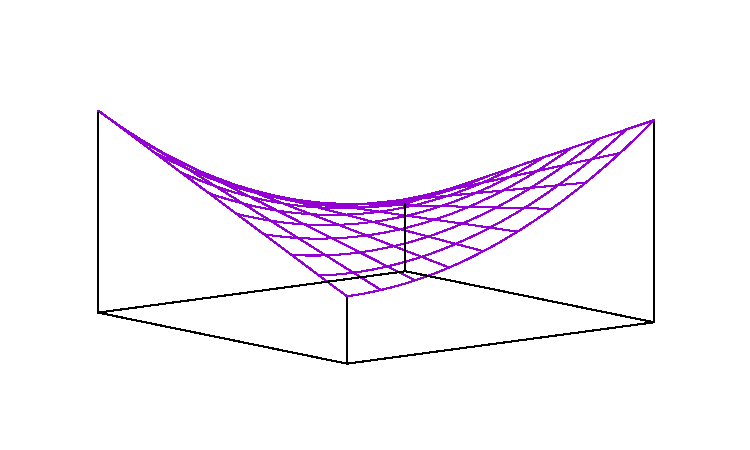
\includegraphics[width=.8\textwidth]{mixed/graph/saddle}
  \caption{The energy surface of a saddle-point system}
  \label{fig:saddle}
\end{figure}

\begin{Definition}{schur-complement}
  Let the operator $A:V\to V^*$ in the saddle-point system be
  invertible. Then, we define the \define{Schur complement} operator
  $S\colon Q\to Q^*$ of the system as
  \begin{gather}
      S= -B A^{-1} B^T - C.
  \end{gather}
\end{Definition}

\begin{Lemma}{schur-complement1}
  Formally, the saddle-point system~\eqref{eq:saddle-point-operator}
  can be solved in two steps by solving
  \begin{align}
    S p &= g - B A^{-1} f,\\
    A u &= f-B^T p.
  \end{align}
\end{Lemma}

\begin{proof}
  Formally solve the first equation
  of~\eqref{eq:saddle-point-operator} for $u$ and enter into the
  second.
\end{proof}

\begin{Lemma}{schur-definiteness}
  Let $a(\cdot,\cdot)$ be elliptic and $c(\cdot,\cdot)$ be positive semi-definite, and
  let $\ker B^T\cap\ker C \neq \{0\}$. Then, the bilinear form
  $\mathcal A(\cdot,\cdot)$ is indefinite.
\end{Lemma}

\begin{proof}
  First, we note that because of ellipticity of $a(\cdot,\cdot)$
  \begin{gather}
    \mathcal A\mixedform(u,0,u,0) = a(u,u) \ge \gamma \norm{u}_V^2,
  \end{gather}
  for some positive constant $\gamma$. Furthermore, $A$ is invertible
  and its inverse is positive definite. Furthermore,
  $A^{-1}B^T\colon Q\to V$. Then, choosing $v=-A^{-1}B^T p$ yields
  \begin{align}
    \mathcal A\mixedform(v,p,v,p)
    &= a(A^{-1}B^T p,A^{-1}B^T p) - 2b(A^{-1}B^T p,p) - c(p,p) \\
    &= \scal(B^T p,A^{-1}B^T p) - 2\scal(B^T p,A^{-1}B^T p) - c(p,p)\\
    &= -\scal(B^T p,A^{-1}B^T p) - c(p,p).
  \end{align}
  The first term is a quadratic term with the bilinear form associated
  with $A^{-T}$, which is positive definite. Since $b(\cdot,\cdot)$ is not the
  zero form, there is some $p$ such that $v\neq 0$. Therefore, with
  the minus sign and the semi-definiteness of $c(\cdot,\cdot)$ we have found a
  vector such that
  \begin{gather}
    \mathcal A\mixedform(v,p,v,p) < 0.
  \end{gather}
\end{proof}

\begin{remark}
  The previous result holds in particular for
  $c(\cdot,\cdot) \equiv 0$, if $B^T$ is injective.
\end{remark}

%%% Local Variables: 
%%% mode: latex
%%% TeX-master: "main"
%%% End: 


\section{Relation to constrained minimization}
%%%%%%%%%%%%%%%%%%%%%%%%%%%%%%%%%%%%%%%%%%%%%%%%%%%%%%%%%%%%%%%%%%%%%%
%%%%%%%%%%%%%%%%%%%%%%%%%%%%%%%%%%%%%%%%%%%%%%%%%%%%%%%%%%%%%%%%%%%%%%
\section{Relation to constrained minimization}

\begin{intro}
  We end our introduction by relating the Stokes equations to a
  constrained minimization problem very much like we had considered
  the solution of the Poisson equation as a minimization problem on
  the space $V$.
\end{intro}

\begin{Theorem}{minimization}
  Assume that $a(\cdot,\cdot)$ is symmetric and $V$-elliptic on the Hilbert
  space $V$. Let
  \begin{gather}
    J(v) = \tfrac12 a(v,v) - f(v).    
  \end{gather}
  Then, the minimization problem finding $u\in V$ such that
  \begin{align}
    J(u) =\inf_{v\in V} J(v),
  \end{align}
  has a unique solution, which then is a minimum. It is determined by
  the first order necessary condition
  \begin{gather*}
    a(u,v) = f(v) \quad\forall v\in V.
  \end{gather*}
\end{Theorem}

\begin{intro}
  In the next step, we constrain the solution $u$ to a subspace of $V$
  defined as the kernel of the linear operator $B: V\to Q^*$. Hence,
  we consider the minimization problem
  \begin{gather*}
    J(u) =\min J(v) \quad
    \text{subject to}\quad
    Bu = 0.
  \end{gather*}
  Going back to formulations with bilinear forms, the constraint
  translates to
  \begin{gather}
    u\in \ker B = \bigl\{ v\in V \;\big|\;
    b(v,q)=0 \quad\forall q\in Q\}.
  \end{gather}
  Since $\ker B$ is a vector space, we can just consider the
  restriction of the minimization problem to this space. This is
  called the reduced problem.
\end{intro}

\begin{Definition}{reduced-problem}
  The \define{reduced problem} of the constrained minimization problem
  above is: find $u\in \ker B$, such that
  \begin{gather}
    J(u) =\inf_{v\in \ker B} J(v).
  \end{gather}
\end{Definition}

\begin{Lemma}{reduced-wellposedness}
  If under the assumptions of \blockref{Theorem}{minimization} there
  holds in addition that $\ker B$ is a closed subspace of $V$, then
  the reduced problem in \blockref{Definition}{reduced-problem} has a
  unique solution.
\end{Lemma}

\begin{proof}
  A closed subspace of a Hilbert space is a Hilbert space
  itself. Then, the $V$-ellipticity of $a(\cdot,\cdot)$ is inherited on
  $\ker B$, and thus the Lax-Milgram lemma provides a unique solution
  for the first order necessary condition on $\ker B$.
\end{proof}

\begin{remark}
  Here we already note that $V$-ellipticity of $a(\cdot,\cdot)$ is sufficient,
  but not necessary. Indeed, ellipticity on $\ker B$ would have been
  sufficient for well-posedness of the reduced problem.
\end{remark}

\begin{intro}
  While the solution theory for the reduced problem is particularly
  simple and purely elliptic, the actual solution requires a
  representation of functions in $\ker B$, for instance a basis of
  these functions. In practice, this is often inconvenient, and we
  seek a method that solves a problem on the whole space.
\end{intro}

\begin{Theorem}{lagrange-multiplier}
  If $u\in V$ is a solution of the constrained minimization problem
  \begin{gather*}
    J(u) = \min_{v\in V} J(v), \quad\qquad
    b(u,q) = 0 \quad\forall q\in Q,
  \end{gather*}
  the pair $(u,p)\in V\times Q$ is a stationary point of
  the \define{Lagrange functional}
  \begin{gather}
    \mathscr L(v,q) = \tfrac12 a(v,v) - f(v) + b(v,q).
  \end{gather}
  Here, $p\in Q$ is called the \define{Lagrange multiplier}.
\end{Theorem}

\begin{Problem}{lagrange-multiplier}
  Verify: the first order necessary conditions of the Lagrange
  multiplier rule are
  \begin{gather*}
    \arraycolsep.1em
    \begin{matrix}
      a(u,v) &+& b(v,p) &=& f(v) &\quad&\forall v\in V, \\
      b(u,q) && &=& 0 &&\forall q\in Q.
    \end{matrix}
  \end{gather*}
  To this end, recall the type of objects that derivatives of linear
  functionals are and compute the derivatives of $\mathscr L$.
\end{Problem}

\begin{Corollary}{stokes-lagrange}
  The Stokes equations with no-slip boundary conditiond are the first
  order necessary conditions for the constrained minimization problem:
  find a velocity $u\in V = H^1_0(\domain)$ such that
  \begin{align*}
    \tfrac12\form(\nabla u,\nabla u) - f(u) &= \min,\\
    \form(\div u,q) &= 0 \qquad\forall q\in Q.
  \end{align*}
\end{Corollary}

%%% Local Variables: 
%%% mode: latex
%%% TeX-master: "main"
%%% End: 


\section{Additional problems and experiments}

\begin{Problem}{elasticity-locking-convergence}
  The graph for $\lambda=100$ in \cref{fig:elasticity-locking}
  suggests the following behavior: on very coarse meshes, the solution
  is badly approximated. Eventually, the approximation cathes up and
  is even faster than orer $h^{-1}$ until it approximates
  asymptotically the straight line for $\lambda=1$. The curve for
  $\lambda=1000$ seems to show the beginning of this behavior.

  \begin{enumerate}
  \item Compute on finer meshes to see if this is actually true. If
    such a behavior is confirmed, this implies that the part of the
    bilinear form with $\lambda$ is less important on finer meshes,
    something which cannot be covered by Céa's lemma from the elliptic
    toolbox.
  \item Compute the energy norm of the error as in the symmetric
    finite element toolbox. What do those curves look like? There, the
    constant in Céa's lemma is 1.
  \item Can we draw any conclusions on the best approximation in the
    energy norm?
  \end{enumerate}
\end{Problem}

\chapter{Conditions for well-posedness}
\label{sec:mixed-wellposedness}
In this chapter, we will first modify conditions for well-posedness in
finite dimensions from positive definiteness to the general case. In
particular, we will derive a quantitative formulation, which we will
study for infinite dimensional problems in the second section. In the
third section, we derive the inf-sup condition for mixed problems as a
special case.

\section{Finite-dimensional problems}
\begin{intro}
  So far, our power horse for well-posedness was the Lax-Milgram
  lemma, which can be applied under the conditions
  \begin{xalignat}2
    a(u,v) &\le M \norm{u}\norm{v} & \forall u,v&\in V\\
    \label{eq:infsup:elliptic}
    a(u,u) &\ge \gamma \norm{u}^2 & \forall u&\in V.
  \end{xalignat}
  The second condition can also be rewritten in terms of the
  \putindex{Rayleigh quotient} as
  \begin{gather*}
    0 < \gamma = \inf_{u\in V}\frac{a(u,u)}{\norm{u}^2}.
  \end{gather*}
  Restricting this to a finite dimensional space, the notation usually
  changes from
  \begin{gather}
    a(u,v) = f(v)
    \qquad\text{to}\qquad
    v^TA u = v^T f,
  \end{gather}
  where $A\in \R^{n\times n}$ is the matrix associated with the
  bilinear form. The bound for the Rayleigh quotient means nothing but
  that the real parts of all eigenvalues of $A$ are bounded from below
  by $\gamma$. Thus, a matrix $A$ for which we can apply the
  Lax-Milgram lemma is positive definite. And the statement of the
  lemma in finite dimension is, that a positive definite matrix is
  invertible. We know from linear algebra that this is true, but we
  also know that the condition is all but necessary.
\end{intro}

\begin{intro}
  Why did we replace this clear theorem by the weaker Lax-Milgram
  lemma, when we studied elliptic partial differential equations?  For
  the first condition, it should be noted that spectral properties of
  operators between spaces of infinite dimension are much harder to
  obtain. Further, we do not need information on the whole spectrum,
  but only on the eigenvalue closest to zero. Therefore, we used a
  simple estimate in order to avoid discussing the spectrum at
  all. But, there is an important difference between
  Theorem~\ref{Theorem:la-invertible} and the
  estimate~\eqref{eq:infsup:elliptic}: the assumption of the theorem
  is qualitative, $\lambda \neq 0$, while the assumption of Lax-Milgram
  is quantitative,
  \begin{gather*}
    \Re\lambda \ge \gamma> 0.
  \end{gather*}
  The following problem shows why such a change is necessary.
\end{intro}

\begin{Problem}{unbounded-inverse}
  On the space $\ell_2(\R)$ define the operator $A$ by its eigenvalue
  decomposition
  \begin{align*}
    A: \ell_2(\R) &\to \ell_2(\R)\\
    e_k & \mapsto \tfrac1k e_k.
  \end{align*}
  Here, $\{e_k\}$ is the orthogonal basis of unit vectors of the form
  \begin{gather*}
    \arraycolsep0.1em
    \begin{array}{cccccccc}
      e_k =(0&,\ldots,&0&,&1&,&0&,\ldots)^T.\\
      &&&&\uparrow\\
      &&&&k
    \end{array}
  \end{gather*}
  \begin{enumerate}
  \item Show that this operator does not have a bounded inverse, albeit
    its eigenvalues are positive.
  \item Show that the range of $A$ is not closed in $\ell_2(\R)$
  \end{enumerate}
\begin{solution}  
  \begin{enumerate}
  \item For each $e_k$, the inverse is $A^{-1} e_k = k e_k$. In particular, $A$ is injective.
    On the other hand, it holds
    \begin{gather*}
      \lim_{k\to\infty}\frac{\norm{A^{-1}e_k}}{\norm{e_k}}=\lim_{k\to\infty}k=\infty
    \end{gather*}
      and the inverse cannot be bounded.
  \item We have to construct a convergent sequence in the range of $A$
    such that the pre-image of the sequence does not converge.
    \begin{enumerate}
    \item Choose
      \begin{gather*}
        v_n = \sum_{k=1}^n \frac1k e_k.
      \end{gather*}
      \item $v_n$ is a Cauchy-sequence, since
        \begin{gather*}
          \norm{v_m-v_n}^2 = \norm*{\sum_{k=m}^n \frac1k e_k}^2
          = \sum_{k=m}^n \frac1{k^2}\norm*{e_k}^2
          \le \frac1{m^2} \sum_{k=1}^\infty \frac1{k^2}
          = \frac{\pi^2}{6} \frac1{m^2}.
        \end{gather*}
      \item We conclude that $v=\lim_{n\to\infty}v_n$ exists in the
        closure of the range of $A$.
      \item There holds
        \begin{gather*}
          v_n = A \sum_{k=1}^n e_k =: A u_n.
        \end{gather*}
      \item Due to the injectivity of $A$ for $v$ to be in the range of $A$,
            $u_n$ has to converge in $\ell_2(\R)$.
      \item The sequence $u_n$ is not a Cauchy sequence, since
        \begin{gather*}
          \norm{v_m-v_n}^2 = \norm*{\sum_{k=m}^n e_k}^2
          = \sum_{k=m}^n \norm*{e_k}^2
          = n-m.
        \end{gather*}
    \end{enumerate}
  \end{enumerate}
\end{solution}
\end{Problem}

\begin{Problem}{lax-milgram-not-applicable}
  Find an invertible, symmetric matrix $A\in \R^{2\times 2}$ and a
  vector $v\in \R^2$ such that $v^T A v=0$ and thus the Lax-Milgram
  lemma is inconclusive.
\begin{solution}
  \begin{gather*}
    A =
    \begin{pmatrix}
      1 & 0 \\ 0 & -1
    \end{pmatrix}
  \end{gather*}
\end{solution}
\end{Problem}

The question of well-posedness in finite dimensions can be answered by:

\begin{Theorem}{la-invertible}
  A matrix $A\in\R^{n\times n}$ is invertible if and only if one of
  the following equivalent conditions holds:
  \begin{enumerate}
  \item all its (possibly complex) eigenvalues are nonzero,
  \item all its singular values are nonzero,
  \item for each $v\in\R^n$ holds $Av\neq 0$.
  \end{enumerate}
\end{Theorem}

\begin{intro}
  We focus on the second and third conditions, respectively, in
  Theorem~\ref{Theorem:la-invertible}.
  But, the problem above tells us that we
  will run into trouble, if we do not quantify this. Therefore, we
  start our attempt by requiring:
  \begin{gather*}
    \norm{Au}^2 \ge \gamma \norm{u}^2 \qquad\forall u\in V.
  \end{gather*}
  But while this is a condition we can easily write down for matrices
  and operators, it does not work that well for bilinear forms. Thus,
  we first look at the singular value decomposition.
\end{intro}

\begin{Theorem}{svd}
  Let $A\in\R^{m\times n}$ be a real matrix. Then, there exist two
  orthogonal matrices $U\in\R^{m\times m}$ and $V\in \R^{n\times n}$
  as well as a real, nonnegative diagonal matrix $\hat\Sigma$, such
  that
  \begin{gather}
    \label{eq:svd:1}
    A = U \Sigma V^\transpose,
    \qquad\text{and }
    \Sigma =
    \begin{cases}
      \begin{bmatrix}
        \hat\Sigma &0
      \end{bmatrix}
      &\text{for } m<n\\
      \hat\Sigma&\text{for } m=n\\
      \begin{bmatrix}
        \hat\Sigma \\0
      \end{bmatrix}
      &\text{for } m>n
    \end{cases}
  \end{gather}
  This is the \define{singular value decomposition} (\define{SVD}) of
  $A$, the diagonal entries of $\hat \Sigma$ are the
  \define{singular values} of $A$ and the column vectors of $U$ and
  $V$ are the left and right \define{singular vectors} of $A$,
  respectively. The same theorem holds for complex matrices with
  unitary $U$ and $V$.
\end{Theorem}

\begin{proof}
  We prove constructively for the real case by induction. For $m=1$ or
  $n=1$ the theorem is obvious. Let now $m,n>1$ and assume the theorem
  has been proven for $A\in \R^{(m-1)\times (n-1)}$. Let $\sigma_1^2$
  be the largest eigenvalue of $A^\transpose A$, which due to the symmetry of
  $A^\transpose A$ is real and nonnegative. Actually, if it is zero, then
  $A^\transpose A=0$ and thus $A=0$ and $\Sigma=0$. Now assume $\sigma_1^2 >
  0$. Choose $x_1$ as an eigenvector to the eigenvalue $\sigma_1^2$ of
  $A^\transpose A$ and
  \begin{gather}
    y_1 = \frac1{\sigma_1} A x_1.
  \end{gather}
  We can complete both $x_1$ and $y_1$ to an orthonormal basis $X$ and
  $Y$, respectively. Then, there holds for $e_1 \in \R^n$ and
  $\bar e_1\in \R^m$:
  \begin{align}
    Y^\transpose AX e_1 &= Y^\transpose A x_1 = \sigma_1 Y^\transpose y_1 = \sigma_1 \bar e_1\\
    (Y^\transpose AX)^\transpose \bar e_1 = X^\transpose A^\transpose Y\bar e_1,
              &= X^\transpose A^\transpose y_1 =  \tfrac1{\sigma_1} X^\transpose A^\transpose A x_1
                = \sigma_1 X^\transpose x_1 = \sigma_1 e_1.
  \end{align}
  Thus,
  \begin{gather}
    Y^\transpose AX =
    \begin{bmatrix}
      \sigma_1 & 0 \\ 0 & \tilde A
    \end{bmatrix}
  \end{gather}
  with $\tilde A\in \R^{(m-1)\times (n-1)}$. By induction, there holds
  $\tilde A = \tilde U \tilde \Sigma \tilde V^\transpose$ with orthogonal
  matrices $U$ and $V$ and $\tilde\Sigma$ of the same form as $\Sigma$
  and both dimensions reduced by 1. Now let
  \begin{gather}
    U = Y
    \begin{bmatrix}
      1 & 0\\ 0& \tilde U
    \end{bmatrix},
    \qquad
    V = X
    \begin{bmatrix}
      1 & 0 \\ 0& \tilde V
    \end{bmatrix},
    \qquad
    \Sigma =
    \begin{bmatrix}
      \sigma_1 & 0 \\ 0 & \tilde\Sigma
    \end{bmatrix}
  \end{gather}
  $U$ and $V$ as the product of orthogonal matrices are orthogonal,
  $\sigma$ has the claimed structure and there holds $A=U\Sigma V^\transpose$.
\end{proof}

\begin{Corollary}{svd-order}
  By the construction of the proof, the singular values are ordered by
  decreasing magnitude,
  \begin{gather}
    \label{eq:svd:2}
    \sigma_1 \ge \sigma_2 \ge \dots \ge \sigma_r > 0.
  \end{gather}
  The number $r$ of nonzero singular values is the dimension of the
  range of the matrix $A$.
\end{Corollary}

%%% Local Variables:
%%% mode: latex
%%% TeX-master: "main"
%%% End:


\begin{Definition}{ker-range-rn}
  \index{ker}
  Let $A: V\to W$ be a linear operator. Then, we define
  the \define{kernel} and the \define{range} of $A$ as
  \begin{align*}
    \ker A &= \bigl\{ v\in V \big| Av = 0\bigr\} \\
    \range A &= \bigl\{ w\in W \big| \;\exists\,v\in V: Av=w\bigr\}.
  \end{align*}
\end{Definition}

\begin{Definition}{orthogonal1}
  Let $V\subset\R^n$ be a subspace. We define the \define{orthogonal
    complement} of $V$ as
  \begin{gather}
    \label{eq:infsup:4}
    V^\perp = \bigl\{w\in \R^n \big| \;\forall\,v\in V \scal(w,v) = 0 \bigr\}.
  \end{gather}
\end{Definition}

\begin{Lemma}{ker-coker-rn}
  Let $A\in \R^{m\times n}$ and $A^T$ its transpose. Then, there holds
  \begin{gather}
    \label{eq:infsup:5}
    \begin{split}
      \ker A &= \range{A^T}^\perp\\
      \range A &= \ker{A^T}^\perp\\
      \ker{A^T} &= \range A^\perp\\
      \range{A^T} &= \ker{A}^\perp
    \end{split}
  \end{gather}
\end{Lemma}

\begin{proof}
  % First, we note that
  % \begin{gather*}
  %   \R^n = \ker A \oplus \ker A^\perp,
  %   \qquad
  %   \R^m = \ker{A^T} \oplus \ker{A^T}^\perp.
  % \end{gather*}
  Let $A=U\Sigma V^T$ be the singular value decomposition of $A$ and
  $r$ be the number of nonzero singular values. Then, the first $r$
  vectors of $U$ span the range of $A$ and the last $n-r$ vectors of
  $V$ span its kernel. Furthermore,
  \begin{gather}
    A^T = \bigl(U\Sigma V^T\bigr)^T = V \Sigma U^T.
  \end{gather}
  Therefore, the first $r$ vectors of V span the range of $A^T$ and
  the last $n-r$ vectors of $U$ span its kernel.
\end{proof}

\begin{Corollary}{ker-coker-iso}
  Let $A\in \R^{m\times n}$ and $A^T$ its transpose. Then, the
  restrictions $A\colon \ker A^\perp \to \range A$ and $A^T\colon
  \ker{A^T}^\perp \to \range{A^T}$ are isomorphisms.
\end{Corollary}

\begin{proof}
  We note that $\dim \range A = \dim \range{A^T}$. Thus, by
  \blockref{Lemma}{ker-coker-rn} the dimensions of domain and range of
  each of the restricted operators are equal, say $\dim \range A =
  r$. The singular value decomposition of the operators is
  \begin{gather*}
    A = U\Sigma V^T \qquad A^T = V\Sigma U^T,
  \end{gather*}
  where all matrices are in $\R^{r\times r}$ and
  \begin{gather*}
    \Sigma = \diag(\sigma_1,\dots,\sigma_r),
  \end{gather*}
  and all singular values are positive. Thus, $A$ and $A^T$ are invertible.
\end{proof}

\begin{Corollary}{svd-infsup}
  Let $r=\dim \ker A^\perp$. Then, for the smallest nonzero singular
  value there holds
  \begin{gather}
    \label{eq:infsup:6}
    \sigma_r
    = \inf_{v\in \ker{A}^\perp} \sup_{w\in \R^m} \frac{w^T A v}{\abs{v}\abs{w}}
    = \inf_{w\in \ker{A^T}^\perp} \sup_{v\in \R^n} \frac{w^T A v}{\abs{v}\abs{w}}.
  \end{gather}
\end{Corollary}

\begin{proof}
  Since the Cauchy-Schwarz inequality turns into an equation if and
  only if the two vectors are coaligned, there holds for any $v\in \R^n$:
  \begin{gather*}
    \sup_{w\in\R^m}\frac{w^T A v}{\abs{w}} = \frac{v^T A^T A v}{\abs{Av}}.
  \end{gather*}
  Therefore,
  \begin{gather*}
    \inf_{v\in \ker{A}^\perp} \sup_{w\in \R^m}
    \frac{w^T A v}{\abs{v}\abs{w}}
    = \inf_{v\in \ker{A}^\perp} \frac{\abs{Av}}{\abs{v}}.
  \end{gather*}
  Now, let $v = \sum \alpha_i v_i$ where $v_i$ are the columns of $V$
  in the SVD of $A$. Then,
  \begin{gather*}
    \abs{Av}^2 = \abs*{A\sum_{i=1}^r \alpha_i v_i}^2
    = \abs*{\sum_{i=1}^r \sigma_i \alpha_i u_i}^2
    = \sum_{i=1}^r \sigma_i^2 \alpha_i^2.
  \end{gather*}
  The quotient
  \begin{gather*}
    \frac{\sum_{i=1}^r \sigma_i^2 \alpha_i^2}{\sum_{i=1}^r \alpha_i^2}
  \end{gather*}
  clearly has its minimum if $\alpha_1 = \dots=\alpha_{r-1} = 0$.
\end{proof}

\begin{Definition}{infsup1}
  A bilinear form $a(\cdot,\cdot)$ on $V\times W$ is said to admit the
  \define{inf-sup condition} or is called \define{inf-sup stable}, if
  there holds
  \begin{gather}
    \label{eq:infsup:1}
    \inf_{u\in V} \sup_{w\in W} \frac{a(u,w)}{\norm{u}_V\norm{w}_W}
    \ge \gamma > 0.
  \end{gather}
\end{Definition}

\begin{remark}
  In this finite dimensional exposition, is clear that $V$ and $W$
  must have the same dimension, and thus $V=W=\R^n$. This will be
  different, when we consider infinite dimensional spaces and indeed
  consider different spaces $V$ and $W$.
\end{remark}

\begin{Lemma}{infsup2}
  The following statements are equivalent to the inf-sup
  condition~\eqref{eq:infsup:1}:
  \begin{gather}
    \label{eq:infsup:2}
    \forall u\in V \;\exists w\in W \;:\; a(u,w) \ge \gamma \norm{u}_V\norm{w}_W
  \end{gather}
  \begin{gather}
    \label{eq:infsup:3}
    \forall u\in V
    \;\exists w\in W \;:\;
    \left\{
    \arraycolsep0.3ex
    \begin{array}{rcl}
      \norm{w}_W &\le&\norm{u}_V\\
      a(u,w) &\ge& \gamma \norm{u}_V^2
    \end{array}
    \right.
  \end{gather}
  \begin{gather}
    \label{eq:infsup:3a}
    \forall u\in V
    \;\exists w\in W \;:\;
    \left\{
    \arraycolsep0.3ex
    \begin{array}{rcl}
      \gamma \norm{w}_W &\le&\norm{u}_V\\
      Aw &=& u
    \end{array}
    \right.
  \end{gather}
\end{Lemma}

\begin{Problem}{inf-sup-equivalence}
  Prove \blockref{Lemma}{infsup2}.
\end{Problem}


%%%%%%%%%%%%%%%%%%%%%%%%%%%%%%%%%%%%%%%%%%%%%%%%%%%%%%%%%%%%%%%%%%%%%%
%%%%%%%%%%%%%%%%%%%%%%%%%%%%%%%%%%%%%%%%%%%%%%%%%%%%%%%%%%%%%%%%%%%%%%
\section{Infinite dimensional Hilbert spaces}
%%%%%%%%%%%%%%%%%%%%%%%%%%%%%%%%%%%%%%%%%%%%%%%%%%%%%%%%%%%%%%%%%%%%%%
%%%%%%%%%%%%%%%%%%%%%%%%%%%%%%%%%%%%%%%%%%%%%%%%%%%%%%%%%%%%%%%%%%%%%%

\begin{intro}
  In the previous section, we derived quantitative conditions to
  ensure the invertibility of a matrix $A$ or its restriction to its
  cokernel $\ker A^\perp$. The arguments there have a natural
  extension to infinite dimensional Hilbert spaces, which we will
  derive in this section. We already saw in
  \blockref{Problem}{unbounded-inverse} that we may run into trouble
  if the range of $A$ is not closed. On the other hand, it turns out
  that most notions of linear algebra related to orthogonality can be
  maintained in Hilbert spaces if closed subspaces are considered.
  We begin by citing the most important results.
\end{intro}

\begin{Definition}{polar-orthogonal}
  Let $W\subset V$ be a subspace of a Hilbert space $V$. We define its
  \define{polar space} $W^0\subset V^*$ and its
  \define{orthogonal complement} $W^\perp\subset V$ by
  \begin{gather}
    \label{eq:infsup:7}
    \begin{split}
    W^0 &= \bigl\{f\in V^* \big| \scal(f,w)_{V^*\times V} = 0
    \quad\forall\,w\in W\bigr\},
    \\
    W^\perp &= \bigl\{v\in V \big| \scal(v,w)_{V} = 0
    \quad\forall\,w\in W\bigr\}.
    \end{split}
  \end{gather}
  For a subspace $U\subset V^*$, we define its polar space
  \begin{gather}
    U^0 = \bigl\{v\in V \big| \scal(u,v)_{V^*\times V} = 0
    \quad\forall\,u\in U\bigr\}
  \end{gather}
\end{Definition}

\begin{Lemma}{orthogonal-closed}
  The polar space $W^0$ and the orthogonal complement $W^\perp$ of a
  subspace $W\subset V$ are both closed. So is the polar space $U^0$
  of a subspace $U\subset V^*$.
\end{Lemma}

\begin{proof}
  Consider the mapping
  \begin{align*}
    \Phi_w\colon V^* &\to \R,\\
    v&\mapsto \scal(v,w)_{V^*\times V}.
  \end{align*}
  For any $w$, the kernel of $\phi$ is closed as
  the pre-image of a closed set. $W^0$ is closed since it is the
  intersection of these kernels for all $w\in W$.

  The inner product is continuous on $V\times V$. Therefore, the
  mapping
  \begin{align*}
    \phi_w\colon V &\to \R,\\
    v&\mapsto \scal(v,w),
  \end{align*}
  is continuous. The argument continues as above. Similar for $U^0$.
\end{proof}

\begin{Theorem}{orthogonal-complement}
  Let $W$ be a subspace of a Hilbert space $V$ and $W^\perp$ its
  orthogonal complement. Then, $W^\perp = \overline{W}^\perp$. Further,
  $V = W \oplus W^\perp$ if and only if $W$ is closed.
\end{Theorem}

\begin{proof}
  Clearly, $\overline{W}^\perp \subset W^\perp$ since
  $W\subset\overline{W}$. Let now $u\in W^\perp$. Then, $\phi =
  \scal(u,\cdot)$ is a continuous linear functional on $V$. Therefore,
  if a sequence $w_n \subset W$ converges to $w\in \overline{W}$, we
  have
  \begin{gather*}
    \scal(u,w) = \lim_{n\to\infty} \scal(u,w_n) = 0.
  \end{gather*}
  Hence, $u\in \overline{W}^\perp$ and $W^\perp = \overline{W}^\perp$.

  Now, the ``only if'' follows by the fact, that if $W$ is not
  closed, there is an element $w\in \overline{W}$ but not in $W$ such that
  $\scal(w,u)=0$ for all $u\in W^\perp$. Thus, $w\not\in W^\perp$ and
  consequently $w\not\in W^\perp \oplus W$.

  Let now $W$ be closed. We show that there is a unique decomposition
  \begin{gather}
    \label{eq:infsup:8}
    v = w + u,\qquad w\in W, \;u\in W^\perp,
  \end{gather}
  which is equivalent to $V = W \oplus W^\perp$. Uniqueness follows,
  since
  \begin{gather*}
    v = w_1+u_1 = w_2+u_2
  \end{gather*}
  implies that for any $y\in V$
  \begin{gather*}
    0 = \scal(w_1-w_2+u_1-u_2,y) = \scal(w_1-w_2,y) + \scal(u_1-u_2,y).
  \end{gather*}
  Choosing $y=u_1-u_2$ and $w_1-w_2$ in turns, we see that one of the
  inner products vanishes for orthogonality and the other implies that
  the difference is zero.

  If $v\in W$, we choose $w=v$ and $u=0$. For $v\not\in W$, we prove
  existence by considering that due to the closedness of $W$ there holds
  \begin{gather*}
    d=\inf_{w\in W} \norm{v-w} >0.
  \end{gather*}
  Let $w_n$ be a minimizing sequence. Using the parallelogram identity
  \begin{gather*}
    \norm{a+b}^2+\norm{a-b}^2 = 2\norm{a}^2+2\norm{b}^2,
  \end{gather*}
  we prove that $\{w_n\}$ is a Cauchy sequence by
  \begin{align*}
    \norm{w_m-w_n}^2 &= \norm{(v-w_n)-(v-w_m)}^2\\
    &= 2\norm{v-w_n}^2+2\norm{v-w_m}^2-\norm{2v-w_m-w_n}^2\\
    &= 2\norm{v-w_n}^2+2\norm{v-w_m}^2-4\norm*{v-\frac{w_m+w_n}2}^2\\
    &\le 2\norm{v-w_n}^2+2\norm{v-w_m}^2-4d^2,
  \end{align*}
  since $(w_m+w_n)/2\in W$ and $d$ is the infimum. Now we use the
  minimizing property to obtain
  \begin{gather*}
    \lim_{m,n\to\infty}\norm{w_m-w_n}^2 = 2d^2-2d^2 -4d^2=0.
  \end{gather*}
  By completeness of $V$, $w=\lim w_n$ exists and by the closedness of
  $W$, we have $w\in W$. Let $u=v-w$. By continuity of the norm, we
  have $\norm{u}=d$. It remains to show that $u\in W^\perp$. To this
  end, we introduce the variation $w+\epsilon \tilde w$ with $\tilde
  w\in W$ to obtain
  \begin{align*}
    d^2 &\le \norm{v-w-\epsilon \tilde w}^2\\
    &= \norm{u}^2-2\epsilon\scal(u,\tilde w)+\epsilon^2 \norm{\tilde w},
  \end{align*}
  implying for any $\epsilon>0$
  \begin{gather*}
    0\le-2\epsilon\scal(u,\tilde w)+\epsilon^2 \norm{\tilde w},
  \end{gather*}
  which requires $\scal(u,\tilde w) = 0$.
\end{proof}

\begin{Definition}{orthogonal-projection}
  Let $V$ be a Hilbert space and $W\subset W$ be a closed
  subspace. For a vector $v\in V$, let $v=w+u$ be the unique
  decomposition with $w\in W$ and $u\in W^\perp$. Then we call $w$ and
  $u$ the \define{orthogonal projection}s of $v$ into $W$ and $W^\perp$,
  respectively. We write
  \begin{gather*}
    \Pi_W = w, \qquad \Pi_{W^\perp} = u.
  \end{gather*}
\end{Definition}

\begin{Lemma}{polar-orthogonal-hilbert}
  Let $V$ be a Hilbert space and $W\subset W$ be a closed
  subspace. Then, the polar space $W^0\subset V^*$ and the orthogonal
  space $W^\perp$ can be isometrically identified by \putindex{Riesz
    representation}.
\end{Lemma}

\begin{proof}
  For every $f$ in the
  dual of $W^\perp$, define $g\in V^*$ by
  \begin{gather*}
    \scal(g,v)_{V^*\times V} =
    \scal(f,\Pi_{V^\perp}v)_{(V^\perp)^*\times V^\perp}.
  \end{gather*}
  Clearly, $g(v)=0$ for $v\in W$, therefore $g\in W^0$.
\end{proof}

% \begin{Corollary}
  
% \end{Corollary}


\begin{Theorem}{closed-range}
  Let $V,W$ be Hilbert spaces and $A\colon V\to W$ a continuous linear
  operator. Then, the following statements are equivalent:
  \begin{gather}
    \label{eq:infsup:9}
    \begin{split}
      \range A &\text{is closed in } W,\\
      \range{A^T} &\text{is closed in } V^*,\\
      \range A &= \ker{A^T}^0,\\
      \range{A^T} &= \ker{A}^0.
    \end{split}
  \end{gather}
\end{Theorem}

\begin{remark}
  This is the famous \emph{\putindex{closed range theorem}} by Banach.
  It actually holds under weaker assumptions, for instance $V,W$ only
  Banach spaces. The proof can be found for instance
  in~\cite[p.~205--209]{Yosida80}.
\end{remark}

\begin{Theorem}{open-mapping}
  Let $A\colon V\to W$ be continuous and surjective. Then, the image
  $A(U)\subset W$ of any open set $U\subset V$ is open.
\end{Theorem}

\begin{remark}
  This is the \emph{\putindex{open mapping theorem}} by Banach. The
  proof can be found for instance in~\cite[p.75--76]{Yosida80}.
\end{remark}

\begin{Lemma}{closed-infsup}
  Let $A\colon V\to W$ be continuous. Then, $\range A$ is closed in
  $W$ if and only if there exists $\gamma>0$ such that
  \begin{gather}
    \label{eq:infsup:10}
    \forall \,w\in W\;
    \exists \,v\in V\quad
    Av = w
    \;\wedge\;
    \gamma \norm{v}_V \le \norm{w}_W.
  \end{gather}
\end{Lemma}

\begin{proof}
  We first show that the inf-sup condition~\eqref{eq:infsup:10}
  implies $\range A$ closed. To this end, let $\{w_n\}$ be a Cauchy
  sequence in $\range A$ converging to a point $w\in W$. Thus, there
  is a sequence $\{v_n\}$ in $V$ such that $Av_n = w_n$ and
  $\gamma \norm{v_n} \le \norm{w_n}$. Hence,
  \begin{gather*}
    \norm{v_m-v_n}_V \le \frac1\gamma \norm{w_m-w_n}_W,
  \end{gather*}
  and $\{v_n\}$ is a Cauchy sequence in $V$. Therefore, $v_n\to v\in
  V$ and due to continuity of $A$ we obtain $Av=w$ and thus $w\in
  \range A$.

  Conversely, let $\range A$ be closed in $W$. Thus, it is a Banach
  space and the \putindex{open mapping theorem} applies to $A\colon
  V\to\range A$. We map the open unit ball $B_1(0)\subset V$ and
  obtain that $A(B_1(0))$ is open in $\range A$, implying that there
  is an open ball $B_\delta(0) \subset A(B_1(0))$. This is sufficient
  to construct $v$:

  Let $w\in\range A$. Then,
  \begin{gather*}
    \tilde w\frac\delta2 \frac{w}{\norm{w}} \in B_\delta(0) \subset A(B_1(0)).
  \end{gather*}
  Hence, there is $v\in V$ with $\norm{v}<1$ such that $Av=\tilde w$,
  which proves the lemma.
\end{proof}

\begin{Theorem}{infsup-well-equivalence}
  Let $a(\cdot,\cdot)$ on $V\times W$ be a bounded bilinear form such that
  \begin{gather}
    a(v,w) \le M \norm{v}_V \norm{w}_W,
  \end{gather}
  and $A\colon V\to W^*$ its associated operator.
  Then, the following statements are equivalent:
  \begin{enumerate}
  \item There exists $\gamma>0$ such that
    \begin{gather}
      \label{eq:infsup:11}
      \inf_{w\in W}\sup_{v\in V}
      \frac{a(v,w)}{\norm{v}_V\norm{w}_W}
      \ge \gamma.
    \end{gather}
  \item The operator $A^T\colon W\to \ker A^0$ is an isomorphism and
    \begin{gather}
      \label{eq:infsup:12}
      \norm{A^Tw}_{V^*} \ge \norm{w}_{W} \qquad\forall w\in W.
    \end{gather}
  \item The operator $A\colon \ker A^\perp\to W^*$ is an isomorphism
    and
    \begin{gather}
      \label{eq:infsup:13}
      \norm{Av}_{W^*} \ge \gamma\norm{v}_V\qquad \forall v\in \ker A^\perp.
    \end{gather}
  \end{enumerate}
\end{Theorem}

\begin{proof}
  First, we show the equivalence of the first two statements. Let us
  rephrase the inf-sup condition to
  \begin{gather*}
    \norm{A^T w}_{V^*}
    = \sup_{v\in V}\frac{\scal(A^T w,v)}{\norm{v}_V}
    = \sup_{v\in V}\frac{a(v,w)}{\norm{v}_V}
    \ge \gamma\norm{w} \qquad
    \forall w\in W.
  \end{gather*}
  Thus, equations~\eqref{eq:infsup:11} and~\eqref{eq:infsup:12} are
  equivalent and we have already proven that the second statement
  implies the first. It remains to show the $A^T$ is an isomorphism
  from $W$ onto $\ker A^0$. Equation~\eqref{eq:infsup:12} implies that
  $A^T\colon W \to \range{A^T}$ is an isomorphism and its inverse is
  bounded by $1/\gamma$ (multiply both sides by $A^{-1}$). Using
  \blockref{Lemma}{closed-infsup}, we obtain that $\range{A^T}$ is
  closed in $V^*$ and the \putindex{closed range theorem} settles the
  issue.

  In order to prove equivalence of the second and third statement, we
  use \blockref{Lemma}{polar-orthogonal-hilbert} to isometrically
  identify $(\ker A^\perp)^*$ with $\ker A^0$. Thus, $A$ is an
  isomorphism from $\ker A^\perp$ onto $W$ if and only if $A^T$ is an
  isomorphism from $W$ onto $(\ker A^\perp)^* = \ker A^0$. and
  \begin{gather*}
    \norm{A}_{W^*\to \ker A^\perp} = \norm{A^T}_{\ker A^0\to W}.
  \end{gather*}
\end{proof}

\begin{Corollary}{infsup-well-posedness1}
  Let $a(\cdot,\cdot)$ on $V\times W$ be a bounded bilinear form such that
  \begin{gather}
    a(v,w) \le M \norm{v}_V \norm{w}_W.
  \end{gather}
  Let the inf-sup-condition
  \begin{gather*}
    \inf_{w\in W}\sup_{v\in V}
    \frac{a(v,w)}{\norm{v}_V\norm{w}_W}
    \ge \gamma > 0    
  \end{gather*}
  hold.  Then, the problem finding $w\in W$ such that
  \begin{gather*}
    a(v,w) = f(v) \qquad\forall v\in V,
  \end{gather*}
  has a unique solution for $f\in \ker A^0$ and
  \begin{gather}
    \norm{w}_W \le \frac1\gamma \norm{f}_{V^*}.
  \end{gather}
\end{Corollary}

\begin{remark}
  \blockref{Theorem}{infsup-well-equivalence} exhibits an asymmetry
  between the left and right argument. In particular, we obtain a
  unique solution only for the adjoint operator $A^T$, which is
  exactly what we need, when we compute say a pressure from the
  divergence of a velocity field. In general, we consider the
  restriction of $f$ to the polar set of the kernal in the above
  well-posedness result detrimental and would prefer a result that
  holds for all $f\in V^*$. This on the other hand requires
  $\ker A=\{0\}$, or $\overline{\range{A^T}} = W^*$. Then, on the
  other hand, we see that $\range{A^T}$ is closed since $\range{A}$ is
  closed and the closed range theorem holds. Therefore, we obtain the
  following theorem for the case that we require a unique solution for
  all right hand sides.
\end{remark}

\begin{Theorem}{infsup-well-posedness2}
  Let $a(\cdot,\cdot)$ on $V\times W$ be a bounded bilinear form such that
  \begin{gather}
    a(v,w) \le M \norm{v}_V \norm{w}_W.
  \end{gather}
  Let for some $\gamma>0$ the inf-sup-conditions
  \begin{align*}
    \inf_{w\in W}\sup_{v\in V}
    \frac{a(v,w)}{\norm{v}_V\norm{w}_W}
    &\ge \gamma,\\
    \inf_{v\in V}\sup_{w\in W}
    \frac{a(v,w)}{\norm{v}_V\norm{w}_W}
    &\ge \gamma
  \end{align*}
  hold.  Then, the problem finding $v\in V$ such that
  \begin{gather*}
    a(v,w) = f(w) \qquad\forall w\in W,
  \end{gather*}
  has a unique solution for $f\in W^*$ and
  \begin{gather}
    \norm{v}_V \le \frac1\gamma \norm{f}_{W^*}.
  \end{gather}  
\end{Theorem}

\begin{remark}
  If we compare \blockref{Theorem}{infsup-well-posedness2} with
  \blockref{Corollary}{infsup-well-posedness1}, we see that the only
  difference lies in the fact that the second inf-sup condition
  ensures surjectivity of $A$ by injectivity of $A^T$. In some cases
  it may be difficult to prove both inf-sup conditions. Then, it is
  sufficient to prove one inf-sup condition, say the first, and then
  only
  \begin{gather*}
     \inf_{v\in V}\sup_{w\in W}
    \frac{a(v,w)}{\norm{v}_V\norm{w}_W} > 0,
  \end{gather*}
  thus, injectivity of $A^T$. Although we verify less than the
  assumptions of \blockref{Theorem}{infsup-well-posedness2}, the
  closed range theorem saves us from the additional work. We further
  note that this notion is symmetric between $A$ and $A^T$, that is,
  it is sufficient to prove inf-sup for either operator and
  injectivity for the other.
\end{remark}

%%%%%%%%%%%%%%%%%%%%%%%%%%%%%%%%%%%%%%%%%%%%%%%%%%%%%%%%%%%%%%%%%%%%%%
%%%%%%%%%%%%%%%%%%%%%%%%%%%%%%%%%%%%%%%%%%%%%%%%%%%%%%%%%%%%%%%%%%%%%%
\section{The inf-sup condition for mixed problems}
%%%%%%%%%%%%%%%%%%%%%%%%%%%%%%%%%%%%%%%%%%%%%%%%%%%%%%%%%%%%%%%%%%%%%%
%%%%%%%%%%%%%%%%%%%%%%%%%%%%%%%%%%%%%%%%%%%%%%%%%%%%%%%%%%%%%%%%%%%%%%

\begin{intro}
  In the previous section, we have developed a framework for
  well-posedness of problems which are not $V$-elliptic. In principle,
  this theory can be applied to the bilinear form
  $\mathcal A((u,p),(v,q))$ as a whole. On the other hand, we can
  formally split the solution of a constrained minimization problem
  into the reduced problem and then computing the Lagrange multiplier,
  which more clearly exhibits the relation of the two spaces $V$ and
  $Q$ involved in the mixed formulation. Here are the resulting
  theorems.
\end{intro}

\begin{Theorem}{infsup-mixed1}
  Let $V$ and $Q$ be Hilbert spaces and let the mixed bilinear form
  \begin{gather*}
        \mathcal A\mixedform(u,p,v,q)
      = a(u,v) + b(v,p) + b(u,q)
  \end{gather*}
  be defined and bounded for any $u,v\in V$ and $p,q\in Q$.
  Then, the problem
  \begin{gather*}
    \mathcal A\mixedform(u,p,v,q) = \scal(f,v)+\scal(g,q)
    \quad\forall v\in V, q\in Q,
  \end{gather*}
  has a unique solution for any $f\in V^*$ and any $g\in Q^*$ if and
  only if there exists $\gamma>0$ such that
  \begin{gather*}
    \forall
    \begin{bmatrix}
      u\in V\\p\in Q
    \end{bmatrix}
    \;
    \exists
    \begin{bmatrix}
      v\in V\\q\in Q
    \end{bmatrix}
    \colon
    \quad
    \mathcal A\mixedform(u,p,v,q) \ge \gamma
    \norm{(u,p)}_{V\times Q}\norm{(v,q)}_{V\times Q},
  \end{gather*}
  and vice versa.
\end{Theorem}

\begin{proof}
  Straight application of \blockref{Theorem}{infsup-well-posedness2}.
\end{proof}

\begin{Theorem}{infsup-mixed2}
  Let $V$ and $Q$ be Hilbert spaces and let
  \begin{gather}
    \begin{split}
      \ker B &= \bigl\{v\in V \big| b(v,q) = 0 \;\forall q\in Q\bigr\}.
    \end{split}
  \end{gather}
  Then, the problem finding $(u,p)\in V\times Q$ such that
  \begin{gather}
    a(u,v) + b(v,p) + b(u,q) = f(v)+g(q) \quad\forall v\in V, q\in Q,
  \end{gather}
  is well-posed if and only if the problem finding $u\in \ker B$ such that
    \begin{gather}
      a(u,v) = f(v) \quad\forall v\in \ker B
    \end{gather}
    is well-posed and there is a positive constant $\beta$ such that
    \begin{gather}
      \inf_{q\in Q}\sup_{v\in V} \frac{b(v,q)}{\norm{v}_V\norm{q}_Q} \ge \beta.
    \end{gather}
\end{Theorem}

%%%%%%%%%%%%%%%%%%%%%%%%%%%%%%%%%%%%%%%%%%%%%%%%%%%%%%%%%%%%%%%%%%%%%%
%%%%%%%%%%%%%%%%%%%%%%%%%%%%%%%%%%%%%%%%%%%%%%%%%%%%%%%%%%%%%%%%%%%%%%
\section{Galerkin approximation of mixed problems}
%%%%%%%%%%%%%%%%%%%%%%%%%%%%%%%%%%%%%%%%%%%%%%%%%%%%%%%%%%%%%%%%%%%%%%
%%%%%%%%%%%%%%%%%%%%%%%%%%%%%%%%%%%%%%%%%%%%%%%%%%%%%%%%%%%%%%%%%%%%%%



%%% Local Variables: 
%%% mode: latex
%%% TeX-master: "main"
%%% End: 


\chapter{The Stokes problem}
\label{cha:stokes}

\section{Well-posedness of the continuous problem}

\begin{intro}
  We begin our investigation into the Stokes problem by investigating
  the well-posedness of the continuous problem. This is particularly
  simple, since we have
  \begin{gather*}
    a(u,v) = \form(\strain u,\strain v)
  \end{gather*}
  for the original Stokes problem in \blockref{Definition}{stokes-eq1}
  and
  \begin{gather*}
    a(u,v) = \form(\nabla u,\nabla v)
  \end{gather*}
  for the simplified \putindex{Stokes equations} in
  \blockref{Definition}{stokes-eq2}. From the standard theory for the
  Laplacian, we know that the second one is $V$-elliptic on
  $V=H^1_0(\domain;\R^d)$. For the first one, we conclude this by using a
  \putindex{Korn inequality}. Therefore, we can already conclude a
  first result:
\end{intro}

\begin{Lemma}{stokes-a-elliptic}
  Let $V=H^1_0(\domain, \R^d)$ and $V_h\subset V$ a finite dimensional
  subspace. Then, $a(.,.)$ is elliptic on $\ker B$ and on $\ker{B_h}$
  independent of the choices of $Q$ and $Q_h$.
\end{Lemma}

\begin{remark}
  We focus here on no-slip boundary condition on the whole boundary as
  the exemplary case. Other boundary conditions are possible, but as
  soon as the Dirichlet boundary for one velocity component becomes
  too small, the ellipticity of $a(.,.)$ on $V$ must be established by
  new arguments known for instance for Robin boundary conditions. In
  the extreme case of natural boundary conditions all around, $V$ is
  the subspace of $H^1(\domain, \R^d)$ obtained by dividing by the
  space of all translations for the simplified form and by the space
  of all rigid body movements.

  Note that we have established already in
  \blockref{Lemma}{divergence-compatibility} that the condition
  $V=H^1_0(\domain, \R^d)$ implies the reduction of the pressure to
  the space $Q = L^2_0(\domain)$ from
  \blockref{Notation}{pressure-constant}.
\end{remark}

\begin{intro}
  The previous lemma guarantees well-posedness of the
  \putindex{reduced problem} in all possible cases. Therefore, the
  remainder of this section is only concerned with the inf-sup
  condition for the divergence operator. We
  follow~\cite{GiraultRaviart86} in this presentation.
\end{intro}

\begin{Lemma}{stokes-helmholtz}
  Let $V=H^1_0(\domain,\R^d)$. Then, the divergence operator
  $\div\colon V \to L^2(\domain)$ is continuous and the subspace
  \begin{gather*}
    V^0 = \ker \div
    = \bigl\{v\in V \big|
    \div v = 0 \text{ a.e.} \bigr\}
  \end{gather*}
  is closed in $V$ and $V$ admits the orthogonal decomposition
  \begin{gather*}
    V = V^0\oplus V^\perp.
  \end{gather*}
\end{Lemma}

\begin{proof}
  We have that
  \begin{gather*}
    \norm{\div v}_{L^2(\domain)}^2
    = \int_\domain \left(\sum \d_iv_i\right)^2\dx
    \le d \int_\domain \sum \abs{\d_iv_i}^2\dx
    \le d \norm{v}_{H^1(\domain;\R^d)}^2.
  \end{gather*}
  Thus, the divergence operator is a continuous mapping from $V$ to
  $L^2(\domain)$. The definition of $V^0$ is equivalent to the
  definition of zero in $L^2(\domain)$. Finally, since the kernel is
  the pre-image of a closed set under a continuous map, it is
  closed. The existence of the decomposition follows from
  \blockref{Theorem}{orthogonal-complement}.
\end{proof}

\begin{Lemma}{stokes-grad}
  If $f\in V^* = H^{-1}(\domain;\R^d)$ satisfies
  \begin{gather*}
    f(v) = 0 \quad\forall v\in V^0,
  \end{gather*}
  then, there exists $p\in L^2(\domain)$ such that
  \begin{gather*}
    f = \nabla p.
  \end{gather*}
  If $\domain$ is connected, then $p$ is unique up to an additive
  constant.
\end{Lemma}

\begin{proof}
  First, we identify $L^2(\domain)$ with its dual. Then, by
  \begin{gather*}
    \scal(-\nabla p, v)_{V^*\times V}
    = \scal(p, \div v)_{L^2(\domain)},
    \qquad\forall v\in V,
  \end{gather*}
  we see that $-\nabla\colon L^2(\domain)\to V^*$ is the dual to the
  divergence operator. Using the Cauchy-sequence argument, we see that
  $\range{\div}$ is closed in $L^2(\domain)$ and the closed range
  theorem applies. Thus, $\range{-\nabla}$ is closed in $V^*$ and
  \begin{gather*}
    \range{\nabla} = \polar{(V^0)} \cong V^\perp
  \end{gather*}
  is the polar set of the kernel $V^0$. This implies the statement
  that there is a $p$ for every $f$. Uniqueness follows by the fact
  that the only differentiable functions on a connected domain with
  $\nabla p=0$ are the constant functions, and by density of such
  functions in $L^2(\domain)$.
\end{proof}

\begin{Corollary}{stokes-iso}
  Let $\domain$ be connected. Then,
  \begin{enumerate}
  \item $\nabla\colon L^2_0(\domain) \to V^0$ is an isomorphism
  \item $\div\colon V^\perp \to L^2_0(\domain)$ is an isomorphism
  \end{enumerate}
\end{Corollary}

\begin{Theorem}{stokes-infsup}
  Let $\domain\subset \R^d$ be a Lipschitz-domain,
  $V=H^1_0(\domain,\R^d)$ and $Q=L^2_0(\domain)$. Then, there is a
  constant $\beta>0$ depending only on the geometry of $\domain$ such
  that
  \begin{gather}
    \label{eq:stokes:1}
    \inf_{q\in Q}\sup_{v\in V}\frac{\form(\div
      v,q)}{\norm{v}_V\norm{q}_Q} \ge \beta.
  \end{gather}
  Furthermore, the problem finding $(u,p)\in V\times Q$ such that
  \begin{gather}
    \label{eq:stokes:3}
    a(u,v)+\form(\div v,p)+\form(\div u,q) = f(v)+g(q)
    \quad\forall v\in V, q\in Q,
  \end{gather}
  has a unique solution for any right hand side $f\in V^*$ and $g\in
  \range{\div}$.
\end{Theorem}

\section{Stable discretizations}

\begin{intro}
  We begin by application of the generic theory of the previous
  chapter to the Stokes problem in order to obtain a generic error
  estimate based on the concrete choice of norms and a single
  assumption. Guided by this theorem, we spend the remaining part of
  this section exploring different options for the discrete spaces.
\end{intro}

\begin{Theorem}{stokes-convergence}
  Let $V=H^1_0(\domain;\R^d)$ and $Q=L^2_0(\domain)$. Let furthermore
  $V_h\subset V$ and $Q_h\subset Q$ be discrete subspaces such that
  there exists $\beta>0$ independent of $h$ such that
  \begin{gather}
    \label{eq:stokes:2}
    \inf_{q_h\in Q_h}\sup_{v_h\in V_h}\frac{\form(\div
      v_h,q_h)}{\norm{v_h}_V\norm{q_h}_Q} \ge \beta.
  \end{gather}
  Then, the Galerkin approximation of~\eqref{eq:stokes:3} admits a
  unique solution $(u_h, p_h)\in V_h\times Q_h$ with the
  quasi-bestapproximation property
  \begin{gather}
    \label{eq:stokes:4}
    \begin{split}
      \norm{u-u_h}_1
      &\le c_1 \inf_{v_h\in V_h}\norm{u-v_h}_1
      + c_2 \inf_{q_h\in Q_h}\norm{p-q_h}_0
      \\
      \norm{p-p_h}_1
      &\le c_3 \inf_{v_h\in V_h}\norm{u-v_h}_1
      + c_4 \inf_{q_h\in Q_h}\norm{p-q_h}_0.
    \end{split}
  \end{gather}
\end{Theorem}

\begin{Corollary}{stokes-convergence2}
  Under the assumptions of \blockref{Theorem}{stokes-convergence},
  let there be in addition interpolation operators $I_{V_h}$ and
  $I_{Q_h}$ such that
  \begin{gather}
    \label{eq:stokes:5}
    \begin{split}
      \norm{u-I_{V_h} u}_1 &\le c h^k \snorm{u}_{k+1} \\
      \norm{p-I_{Q_h} p}_0 &\le c h^k \snorm{p}_{k}.
    \end{split}
  \end{gather}
  Then, there is a constant $c$ independent of the approximation
  spaces such that
  \begin{gather}
    \label{eq:stokes:6}
    \begin{split}
      \norm{u-u_h}_1 &\le c h^k \bigl(\snorm{u}_{k+1} +
      \snorm{p}_{k}\bigr)
      \\
      \norm{p-p_h}_1 &\le c h^k \bigl(\snorm{u}_{k+1} +
      \snorm{p}_{k}\bigr).
    \end{split}
  \end{gather}
\end{Corollary}
\begin{intro}
  We continue showing that the most natural discretizations
  in two dimensions are not inf-sup stable. This holds for the
  discretization using continuous linear or bilinear elements for both
  velocity components and the pressure as well as for continuous
  linear or bilinear velocity functions combined with piecewise
  constant pressure functions.
\end{intro}

\begin{example}
  We begin with a one-dimensional example. Piecewise linear velocity
  and piecewise linear pressure. Both continuous. Then, $\div v_h$ is
  piecewise constant. Consequently, a pressure function which has zero
  mean value on each cell is in the kernel of $B_h$.
  \begin{figure}[tp]
    \centering
    \includegraphics[width=.6\textwidth]{./fig/p1-p1-1d.tikz}
    \caption[Example for the $P_1-P_1$ pair in one
    dimension]{Piecewise linear pressure (\tikz\draw[color=cyan] (0,0)
      -- (1em,0);) and divergence (\tikz\draw[color=red] (0,0)
      -- (1em,0);) of
      piecewise linear velocity.}
    \label{fig:stokes:p1p1-1d}
  \end{figure}
\end{example}

\begin{example}
  Take a patch of four quadrilaterals or triangles meeting in a common
  vertex. Let $\domain$ be the union of these grid cells. Choose
  linear and bilinear shape functions for $V_h$, respectively. Then, $\dim
  V_h = 2$, since we have one interior vertex with one basis function for
  each velocity component. Choose piecewise constant pressure
  functions. Dividing out the global constant, we conclude that $\dim
  Q_h = 3$. Thus, the statement
  \begin{gather*}
    \forall q_h\in Q_h \;\exists v_h\in V_h:
    \quad \norm{v_h}_1 = \norm{q_h}_0
    \;\wedge\; b(v_h, q_h) \ge \beta \norm{q_h}^2
  \end{gather*}
  cannot hold true. Therefore, the inf-sup condition does not hold. In
  fact, $\ker{B_h} = \{0\}$.
  \begin{figure}[tp]
    \centering
    \includegraphics[width=.4\textwidth]{./fig/patch1.tikz}
    \hfill
    \includegraphics[width=.4\textwidth]{./fig/patch2.tikz}
    \caption[Very coarse meshes with Dirichlet boundary.]{Very coarse meshes with Dirichlet boundary. Degrees of freedom for pressure (\tikz\draw[shape pressure] (0,0) circle (1ex);) and for both velocity components(\tikz\draw[shape veloxy] (0,0) circle (1ex);).}
    \label{fig:stokes:example1}
  \end{figure}

  Thus, we conclude that for this combination of shape function
  spaces, there is a mesh such that they are not suited for the
  approximation of the Stokes problem. But, this may be a problem of a
  mesh with too few cells. In fact, asymptotically, a triangular mesh
  contains twice as many vertices as cells, a quadrilateral mesh as
  many. Therefore, $\dim V_h > \dim Q_h$ as soon as the mesh is
  sufficiently fine. Will this be sufficient?
\end{example}

\begin{Problem}{checker-board}
  Let $\domain = (0,1)^2$ be the unit square and let the mesh consist
  of Cartesian squares of side length $1/n$. Choose $V_h \subset V$
  based on bilinear shape functions. Show that the piecewise constant
  pressure function $p_c=\pm 1$ in a checkerboard fashion is in the
  kernel of $B_h^T$, that is
  \begin{gather*}
    b(v_h, p_c) = 0 \quad\forall v_h\in V_h.
  \end{gather*}
\end{Problem}

\subsection{The MINI element}

\begin{Definition}{barycentric-coordinates}
  A simplex $T\in \R^d$ with vertices $x_0,\dots,x_d$ is described by
  a set of $d+1$ \define{barycentric coordinates}
  $\lambda_0,\dots,\lambda_d$ such that
  \begin{xalignat}2
    0\le\lambda_i(x) &\le 1& i&=0,\dots,d;\quad x\in T\\
    \lambda_i(x_j) &= \delta_{ij}& i,j&=0,\dots,d\\
    \sum \lambda_i(x) &= 1.
  \end{xalignat}
\end{Definition}

\begin{remark}
  The functions $\lambda_i(x)$ are the shape functions of the linear
  $P_1$ element on $T$. They allow us to define basis functions on the
  cell $T$ without use of a reference element $\widehat T$.
  
  Note that $\lambda_i\equiv 0$ on the face opposite to the
  vertex $x_i$.
\end{remark}

\begin{example}
  We can use barycentric coordinates to define shape functions on
  simplicial meshes easily, as in
  Table~\ref{tab:barycentric-shapes}.
  \begin{table}[tp]
    \centering
    \begin{tabular}{|c|l|}
      \hline Degrees of freedom
      & Shape functions \\\hline
      \adjustbox{valign=center,margin=3pt}{\includegraphics[width=2cm]{./fig/p1-p.tikz}}
      &
        {\begin{minipage}[b]{6cm}
          \begin{gather*}
            \phi_i = \lambda_i,
            \quad i=0,1,2
          \end{gather*}
        \end{minipage}}
      \\\hline
      \adjustbox{valign=center,margin=3pt}{\includegraphics[width=2cm]{./fig/p2-p.tikz}}
      &
        {\begin{minipage}[b]{6cm}
          \begin{xalignat*}2
            \phi_{ii} &= 2\lambda_i^2 - \lambda_i,
            &i&=0,1,2\\
            \phi_{ij} &= 4\lambda_i\lambda_j
            &j&\neq i
          \end{xalignat*}
        \end{minipage}}
        \\\hline
      \adjustbox{valign=center,margin=3pt}{\includegraphics[width=2cm]{./fig/p3-p.tikz}}
      &
        {\begin{minipage}[b]{6cm}
          \begin{xalignat*}2
          \phi_{iii} &= \tfrac12 \lambda_i(3\lambda_i-1)(3\lambda_i-2)
          &i&=0,1,2\\
          \phi_{ij} &= \tfrac92\lambda_i\lambda_j(3\lambda_j-1)
          &j&\neq i\\
          \phi_0 &= 27\lambda_0\lambda_1\lambda_2
        \end{xalignat*}
        \end{minipage}}
        \\\hline
    \end{tabular}
    \caption{Degrees of freedom and shape functions of simplicial elements
      in terms of barycentric coordinates}
    \label{tab:barycentric-shapes}
  \end{table}  
\end{example}

\begin{Notation}
  We denote by
  \begin{gather}
    \label{eq:stokes:8}
    H^k_h(\mathcal P) =
    \bigl\{ v\in H^k(\Omega) \big\vert
    v_{|\cell} \in \mathcal P \;\forall \cell\in\mesh_h\bigr\}
  \end{gather}
  the finite element space which is based on the shape function space
  $\mathcal P$, the mesh $\mesh_h$ and is a subspace of
  $H^k(\domain)$. Examples are the continuous spaces of piecewise
  polynomials or tensor product polynomials of degree $k$
  \begin{gather*}
    H^1_h(\P_k) \qquad H^1_h(\Q_k),
  \end{gather*}
  and the discontinuous spaces
  \begin{gather*}
    H^0_h(\P_k) \qquad H^0_h(\Q_k).
  \end{gather*}
\end{Notation}

\begin{Definition}{h1-bubble-space}
  An $H^1$-\define{bubble function} on a mesh cell $\cell$ is a
  function $b\in H^1_0(\cell)$. A \define{bubble space} $b_\cell$ on
  $\cell$ is a discrete vector space of such bubble functions.  We
  denote the space of bubble functions on the mesh $\mesh_h$ by
  \begin{gather*}
    B_h(b_\cell) = \bigl\{ v\in H^1(\domain) \big\vert
    v_{|_\cell} \in b_\cell \;\forall \cell\in\mesh_h
    \bigr\}.
  \end{gather*}
  If there is no confusion about the local bubble space $b_T$, we also
  write just $B_h$.
\end{Definition}

\begin{example}
  A bubble function on a triangle $\cell$ is easily defined by
  \begin{gather}
    \label{eq:stokes:7}
    b_3 = \lambda_0\lambda_1\lambda_2.
  \end{gather}
\end{example}

\begin{Definition}{mini-element-p}
  The \define{MINI element} consists of the spaces
  \begin{gather}
    V_h = \bigl(H^1_h(\P_1) \oplus B_h(b_3) \cap V\bigr)^2,
    \qquad
    Q_h = H^1_h(\P_1) \cap Q.
  \end{gather}
  Its degrees of freedom are:
  \begin{center}
    \includegraphics[width=.2\textwidth]{./fig/p-mini-v.tikz}
    \hspace{1cm}
    \includegraphics[width=.2\textwidth]{./fig/p1-p.tikz}
  \end{center}
\end{Definition}

\begin{intro}
  We will show now that the MINI element is indeed inf-sup stable. To
  this end, we construct the \putindex{Fortin projection} according to
  \blockref{Lemma}{fortin}. Since the construction of such a
  projection operator turns out a bit complicated, we first introduce
  a construction principle, which will help us in our further
  analysis. The idea of this principle is separating the interpolation
  into $V_h$ from the preservation of the divergence.
\end{intro}

\begin{Lemma}{fortin-construction-1}
  Let there be operators $\Pi_1,\Pi_2\colon V \to V_h$ such that
  \begin{xalignat}2
    \label{eq:stokes:10}
    \norm{\Pi_1 v}_V &\le c1 \norm{v}_V
    &\forall v&\in V,\\
    \label{eq:stokes:11}
    \norm{\Pi_2(\identity-\Pi_1)v}_V &\le c_2 \norm{v}_V
    &\forall v&\in V,\\
    \label{eq:stokes:12}
    b(v-\Pi_2v,q_h) &= 0
    &\forall v&\in V, \;q_h\in Q_h,
  \end{xalignat}
  with constants $c_1$ and $c_2$ independent of the discretization
  parameter $h$. Then, the operator
  \begin{gather}
    \label{eq:stokes:9}
    \Pi_h = \Pi_1 + \Pi_2 - \Pi_2\Pi_1
  \end{gather}
  is a \putindex{Fortin projection}, that is, it is bounded on $V$ and
  \begin{gather*}
    b(v-\Pi_h v, q_h) =0 \qquad\forall q_h\in Q_h.
  \end{gather*}
\end{Lemma}

\begin{proof}
  Boundedness of $\Pi_h$ is obvious, such that we only focus on
  preservation of the kernel ob $B$:
  \begin{multline*}
    b(v-\Pi_h v,q_h) = b(v-\Pi_1 v - \Pi_2 v + \Pi_2\Pi_1 v, q_h)
    \\
    = b(v-\Pi_2 v, q_h) - b(\Pi_1 v - \Pi_2\Pi_1 v,q_h) = 0-0 = 0.
  \end{multline*}
\end{proof}

\begin{Assumption}{h1-stable-interpolation}
  There exists an $H^1$-stable interpolation operator $I_h:V\to V_h$
  such that for each cell $\cell \in \mesh_h$ there holds for $m=0,1$
  \begin{gather}
    \label{eq:stokes:13}
    \snorm{v-I_h v}_{m,\cell} \le c \sum_{\cell'\cap\cell
      \neq\emptyset} h_{\cell'}^{1-m}\snorm{v}_{1,\cell'},
  \end{gather}
  with a constant $c$ independent of the mesh parameter $h$.
\end{Assumption}

\begin{remark}
  The interpolation operators of Clément, Scott and Zhang, Schöberl or
  Ern and Guermond fullfil these assumptions.
\end{remark}

\begin{Definition}{locally-quasi-uniform}
  A family of meshes $\{\mesh_h\}$ is called \define{locally
    quasi-uniform}, if there is a constant $c$ such that
  \begin{gather}
    \label{eq:stokes:14}
    \forall h
    \;
    \forall \cell,\cell'\in \T_h
    \quad
    \cell\cap\cell'\neq \emptyset
    \Rightarrow
    h_\cell \le c h_{\cell'}.
  \end{gather}
\end{Definition}

\begin{Assumption}{locally-quasi-uniform}
  We assume of all families of meshes that they are shape regular and
  locally quasi-uniform, such that with
  \blockref{Assumption}{h1-stable-interpolation} there holds
  \begin{gather}
    \label{eq:stokes:15}
    \snorm{v-I_h v}_{m,\cell} \le c h_\cell \snorm{v}_{1,\domain_\cell},
  \end{gather}
  where $\Omega_\cell$ is the union of all cells with nonempty
  intersection with $\cell$.
\end{Assumption}

\begin{Theorem}{mini-stability}
  Under \blockref{Assumption}{locally-quasi-uniform},
  the MINI element is inf-sup stable.
\end{Theorem}

\begin{proof}
  We construct a \putindex{Fortin projection} by choosing
  $\Pi_1 = I_h$, where $I_h:V\to \bigl(H^1_h(\P_1)\bigr)^2$ is an
  $H^1$-stable interpolation operator into the standard linear finite
  element space. Now, we construct $\Pi_2: V \to \bigl(B_h\bigr)^2$
  such that for all $q_h\in Q_h$
  \begin{gather*}
    \int_\domain \div(\Pi_2 v-v) q_h \dx
    = \int_\domain (v-\Pi_2v)\cdot\nabla q_h\dx
    = 0.
  \end{gather*}
  Indeed, $\Pi_2 v$ can be chosen on each cell. Since $\nabla q_h$ is
  constant on a cell $\cell$, we choose
  \begin{gather*}
    \int_\cell \Pi_2 v_i \dx
    = \alpha_{\cell,i} \int_\cell b_3\dx
    = \int_\cell v_i\dx,
  \end{gather*}
  where $i=1,2$ enumerates the velocity components. This is possible,
  since the mean value of $b_3$ is strictly positive. Assuming shape
  regularity, we can use the inverse estimate for $b_3$ to obtain
  \begin{gather*}
    \norm{\Pi_2 v}_{1,\cell}
    \le c h_\cell^{-1} \norm{\Pi_2 v}_{0,\cell}
    \le c h_\cell^{-1} \norm{v}_{0,\cell}.
  \end{gather*}
  Finally, we use the estimates for $I_h$ to obtain
  \begin{gather*}
    \norm{\Pi_2 (\identity-\Pi_1) v}_{1,\cell}
    \le c h_\cell^{-1} \norm{v-I_h v}_{0,\cell}
    \le c \snorm{v}_{1,\domain_\cell}.
  \end{gather*}
  Since the number of intersecting of cells of shape regular meshes is
  bounded, the finale term is bounded by $\norm v_{1,\domain}$.
\end{proof}
\section{Nearly incompressible elasticity}

%%% Local Variables:
%%% mode: latex
%%% TeX-master: "main"
%%% End:


\chapter{Mixed formulation of elliptic problems}
\label{cha:darcy}

\section{Modeling diffusion problems}

\begin{intro}
  Diffusion problems arise when a balance law, for instance for mass
  in ground water flow or for energy in temperature conduction is
  coupled with a constitutive equation relating the direction of
  movement to the gradient of the quantity of interest.
\end{intro}

\begin{intro}
  Let $\rho$ be the density of a conserved quantity. Then, for any given
  volume we have the ``mass''
  \begin{gather*}
    m = \int_V \rho\dx.
  \end{gather*}
  Changes of this mass can be due to two processes:
  \begin{enumerate}
  \item Generation of additional mass by a source $g$,
  \item Flow of mass over the boundary of $V$ at a velocity $v$.
  \end{enumerate}
  In formulas, we have
  \begin{gather*}
    \tfrac{d}{d t} m = \int_V g\dx - \oint_{\d V} J\cdot \n \ds,
  \end{gather*}
  also known as \define{Reynolds transport theorem}. Here, $J$ is the
  \define{flux}. The exact form of the flux will be modeled later.
  The formula above is somewhat unwieldy, since it combines volume and
  surface integrals. Therefore, we apply the \putindex{Gauss theorem}
  to obtain
  \begin{gather}
    \label{eq:darcy:2}
    \frac{d}{dt} \int_V \rho\dx = \int_V g\dx - \int_V \div J \dx.
  \end{gather}
  Concentrating and assuming sufficient regularity, we arrive at the
  equation
  \begin{gather}
    \label{eq:darcy:3}
    \d_t \rho + \div J = g.
  \end{gather}
  As before in these notes, we ignore the time dependence and only
  look at stationary limits. In this case, this reduces to
  \begin{gather}
    \label{eq:darcy:4}
    \div J = g.
  \end{gather}
\end{intro}

\begin{example}
  Next we consider constitutive relations between $\rho$ and $J$ such
  that we can complement equation~\eqref{eq:darcy:4} by a second
  equation and obtain a solvable system. To this end, we consider
  thermal diffusion and ground water flow.

  \begin{description}
  \item[Heat conduction:] Here, the conserved quantity is not the
    density $\rho$, but the temperature $T$. \define{Fourier's law}
    states that the flux is proportional to the gradient of the
    temperature, pointing in opposite direction:
    \begin{gather*}
      J = -k\nabla T.
    \end{gather*}
    The constant of proportionality $k$ is the heat conductivity.
  \item[Porous media flow:] The conserved quantity is the amount of
    fluid, represented by the hydraulic head or pressure
    $p$. \define{Darcy's law} says that the flux is the product of the
    hydraulic \define{permeability} of the media and the gradient of the
    pressure:
    \begin{gather*}
      J = -K\nabla p.
    \end{gather*}
    Here, the permeability $K$ is either a positive scalar function or
    a symmetric, positive definite matrix. Note that in the latter
    case, $J$ and $\nabla p$ do not point in the same direction.
    \item[General diffusion processes:] \define{Fick's law} states,
      that the flux of a diffusion process is determined by the
      gradient of the diffusing quantity $p$ by the relation
    \begin{gather*}
      J = -D\nabla p.
    \end{gather*}
    $D$ is the symmetric, positive definite \define{diffusion tensor}.
  \end{description}
\end{example}

\begin{intro}
  From the two equations for $J$, we derive the following system of
  PDE, where we replace the letter $J$ by the more familiar $u$:
  \begin{gather}
    \label{eq:darcy:5}
    \arraycolsep2pt
    \begin{matrix}
      K^{-1} u &+& \nabla p &=& 0 \\
      \div u &&&=& f.
    \end{matrix}
  \end{gather}
  This system is closed by boundary conditions. Let $\Gamma_D$ be the
  Dirichlet boundary and $\Gamma_N$ be the Neumann boundary such that
  $\Gamma_D \cap \Gamma_N = \emptyset$ and
  $\Gamma_D\cup\Gamma_N = \d\domain$. Then, we let
  \begin{gather}
    \label{eq:darcy:6}
    \begin{aligned}
      p(x) &= p^D(x) & x & \in \Gamma_D, \\
      u(x)\cdot\n &= u^N(x)\cdot n & x & \in \Gamma_N.
    \end{aligned}
  \end{gather}

  Following the concept of finding spaces such that we have an inf-sup
  condition, we are looking for a pair with minimal regularity, such
  that we have a stable and bounded inf-sup condition. We begin the
  usual way by multiplying with a test function and integrating:
  \begin{gather}
    \label{eq:darcy:7}
    \arraycolsep2pt
    \begin{matrix}
      \displaystyle\int_\domain K^{-1} u\cdot v\dx
      &+&
      \displaystyle\int_\domain \nabla p \cdot v\dx
      &=& 0 \\
      \displaystyle\int_\domain \div u q\dx
      &&&=&
      \displaystyle\int_\domain f q\dx.
    \end{matrix}
  \end{gather}
  It turns out, we have two immediate options: first, we can integrate
  the first equation by parts, having all derivatives on $u$ and $v$.
  On the other hand, we can integrate by parts in the second equation,
  leaving all derivatives on $p$ and $q$. In the second case,
  we obtain the equation
  \begin{gather*}
    -\int_\domain u\cdot\nabla q\dx + \int_{\d\domain} u\cdot\n q \ds
    = \int_\domain f q\dx.
  \end{gather*}
  Applying the boundary condition, we first follow the recipe of
  elliptic partial differential equations and implement $p=p^D$ as an
  \putindex{essential boundary condition}, that is, the test function
  space has zero trace on $\Gamma_D$. Then, we can swap in $u^N$ for
  $u$ on $\Gamma_N$, such that the boundary term ends up on the right
  hand side.
\end{intro}

\begin{Definition}{primal-mixed}
  The \define{primal mixed formulation} of the mixed diffusion
  problem~\eqref{eq:darcy:5} reads: find $(u,p)\in V\times Q$ such
  that for all $v\in V$ and $q\in Q$ holds
  \begin{gather}
    \label{eq:darcy:8}
    \arraycolsep2pt
    \begin{array}{rcccl}
      \form(K^{-1} u, v) &+& \form( \nabla p, v)
      &=& 0 \\
      -\form(u,\nabla q)
      &&&=& \form(f,q) - \forme(u^N\cdot\n, q)_{\Gamma_N}.
    \end{array}
  \end{gather}
  The spaces are
  \begin{gather}
    \label{eq:darcy:9}
    \begin{split}
      V &= L^2(\domain;\R^d), \\
      Q &= H^1_{\Gamma_D}(\domain) = \bigl\{
      q\in H^1(\domain) \big| \;q_{|\Gamma_D} = 0
      \bigr\}.
    \end{split}
  \end{gather}
\end{Definition}

\begin{remark}
  Since the first equation is tested with the test function $v$ itself
  in all terms, we can eliminate this equation and there holds
  $u= K\nabla p$ in $L^2(\domain;\R^d)$. Entering this into the second
  equation, we obtain the well-known \putindex{primal formulation}
  \begin{gather*}
    \form(K \nabla p,\nabla q) = \form(f,q)
    - \forme(u^N\cdot\n, q)_{\Gamma_N}.
  \end{gather*}
  Just keep in mind that the ``\putindex{natural boundary condition}''
  in this case is
  \begin{gather*}
    K\nabla p\cdot n = 0.
  \end{gather*}
  Hence, the primal mixed formulation does not provide any advantages
  compared to the primal formulation, and we are not going to pursue
  it further.
\end{remark}

\begin{intro}
  Now we return to the first alternative, namely integrating by parts
  in the first equation of~\eqref{eq:darcy:7}:
  \begin{gather*}
    \int_\domain K^{-1} u \cdot v \dx - \int_\domain p \div v\dx
    + \int_{\d\domain} v\cdot \n p\ds = 0.
  \end{gather*}
  Ensuing is a formulation multiplying and integrating the divergences
  of $u$ and $v$, respectively, with functions in $Q$. In order to fit
  this into our standard framework, we have to introduce a new Sobolev
  space. In addition, since $u\cdot\n$ does not appear as a boundary
  integral, we must make this an \putindex{essential boundary
    condition}. Thus, we require that the test functions have zero
  normal trace on $\Gamma_N$ (and justify this below). Note that now
  the Dirichlet condition $p=0$ has become a ``\putindex{natural
    boundary condition}''!
\end{intro}

\begin{Definition}{hdiv}
  Let $\domain \subset \R^d$ be a domain.  We define the
  Sobolev space
  \begin{gather}
    \Hdiv(\domain) = \bigl\{
    v\in L^2(\domain;\R^d) \big\vert
    \div v\in L^2(\domain)\bigr\},
  \end{gather}
  and its inner product
  \begin{gather}
    \scal(u,v)_{\Hdiv} = \form(u,v)_0 + \form(\div u,\div v)_0.
  \end{gather}
  Furthermore, let $C^\infty_{00}(\domain)$ be the space of smooth
  functions with compact support in $\domain$. Then, we define its
  closure in $\Hdiv(\domain)$:
  \begin{gather}
    \Hdiv_0(\domain) = \overline{C^\infty_{00}(\domain)}.
  \end{gather}
  For subset $\Gamma\subset\d\domain$, the space
  $\Hdiv_\Gamma(\domain)$ is defined accordingly (compare to
  $H^1_\Gamma(\domain)$)
\end{Definition}

Using the space $\Hdiv$ and for the moment the assumption, that
$\Hdiv_0$ and $\Hdiv_\Gamma$ serve to set boundary conditions, we can
write down our second weak formulation of the mixed diffusion problem:

\begin{Definition}{dual-mixed}
  The \define{dual mixed formulation} of the mixed diffusion
  problem~\eqref{eq:darcy:5} reads: find $(u,p) \in V\times Q$ such
  that for all $v\in V$ and $q\in Q$ holds
  \begin{gather}
    \label{eq:darcy:10}
    \arraycolsep2pt
    \begin{array}{rcccl}
      \form(K^{-1} u, v) &-& \form(p, \div v)
      &=& \forme(p^D,v\cdot \n)_{\Gamma_D} \\
      \form(\div u, q)
      &&&=& \form(f,q).
    \end{array}
  \end{gather}
  The spaces are
  \begin{gather}
    \label{eq:darcy:11}
    V = \Hdiv_{\Gamma_N}(\domain),
    \qquad
    Q = L^2(\domain).
  \end{gather}
\end{Definition}

\subsection{Properties of $\Hdiv(\domain)$}

\begin{Theorem}{Hdiv-separable}
  Let $\domain$ be a bounded Lipschitz domain. Then, the space
  $C^\infty(\overline\domain;\R^d)$ is dense in $\Hdiv(\domain)$.
\end{Theorem}

\begin{proof}
  % We use the statement, that a subspace $W$ is dense in a space $V$ if
  % and only if all linear functionals vanishing on $W$ also vanish on
  % $V$. Therefore, let $L \in \Hdiv(\domain)^*$. By the
  % \putindex{Riesz representation theorem}, there is
  % $u\in\Hdiv(\domain)$ such that
  % \begin{gather*}
  %   L(v) = \scal(u,v)_{\Hdiv} = \sum_{i=1}^d \scal(u_i,v_i)_0
  %   + \scal(\div u,\div v)_0
  %   \quad\forall v\in \Hdiv(\domain).
  % \end{gather*}
  % Now assume $L(\phi) = 0$ for all $\phi\in
  % C^\infty(\overline\domain;\R^d)$. Let us extend $u$ and $\div u$ outside
  % of the domain $\domain$ by zero. Then, there holds
  % \begin{gather*}
  %   \int_{\R^d} u\cdot \phi \dx + \int_{\R^d}
  % \end{gather*}
  Either by a standard mollifier argument~\cite{AdamsFournier03} or
  following~\cite[Theorem 2.4]{GiraultRaviart86}
\end{proof}

\begin{remark}
  The condition of boundedness entered the assumptions since we use
  the space $C^\infty(\overline\domain)$. It could be dropped, if we
  used a more appropriate space (cf.~\cite[Theorem
  2.4]{GiraultRaviart86}).
\end{remark}

\begin{Theorem}{Hdiv-trace}
  The \putindex{trace operator}
  $\gamma_n\colon C^\infty(\overline\domain;\R^d) \to
  C^\infty(\overline{\d\domain})$
  which maps $v\mapsto v\cdot\n_{|\d\domain}$ can be extended to a
  continuous, linear mapping
  \begin{gather}
    \gamma_n\colon \Hdiv(\domain) \to H^{-1/2}(\d\domain),
  \end{gather}
  where $H^{-1/2}(\d\domain)$ is the dual of $H^{1/2}(\d\domain)$.
\end{Theorem}

\begin{proof}
  Let $q\in C^\infty(\overline\domain)$ and
  $v\in C^\infty(\overline\domain;\R^d)$. Then, there holds
  \putindex{Green's formula}
  \begin{gather*}
    \form(v,\nabla q)_\domain
    + \form(\div v,q)_\domain
    = \forme(v\cdot\n,q)_{\d\domain}.
  \end{gather*}
  Hence,
  \begin{gather*}
    \left\vert\int_{\d\domain} v\cdot \n q \ds \right\vert
    \le \norm{v}_{\Hdiv} \norm{q}_{H^1}.
  \end{gather*}
  Applying the density of $C^\infty(\overline\domain)$ in
  $H^1(\domain)$ and of $C^\infty(\overline\domain;\R^d)$ in
  $\Hdiv(\domain)$, we can let $q$ and $v$ pass to a limit, but the
  inequality holds uniformly.

  Now apply that $H^{1/2}(\d\domain)$ is the trace space of
  $H^1(\domain)$. Therefore, for any $g\in H^{1/2}(\d\domain)$, there
  is a $q\in H^1(\domain)$ such that $q_{|\d\domain} = g$ and
  $\norm{q}_{1;\domain} \le \norm{g}_{1/2;\d\domain}$. We obtain
  \begin{gather*}
    \left\vert\int_{\d\domain} v\cdot \n g \ds \right\vert
    \le \norm{v}_{\Hdiv(\domain)} \norm{g}_{H^{1/2}(\d\domain)}
    \qquad\forall v\in \Hdiv(\domain), g\in H^{1/2}(\d\domain).
  \end{gather*}
  Hence,
  \begin{gather*}
    \norm{v\cdot\n}_{H^{-1/2}(\d\domain)} \le
    \norm{v}_{\Hdiv(\domain)}
    \qquad\forall v\in \Hdiv(\domain).
  \end{gather*}
  Thus, we have proven the continuity of the extension of $\gamma_n$
  to $\Hdiv(\domain)$.
\end{proof}

\begin{remark}
  The trace theorem tells us that our interpretation of the spaces
  $\Hdiv_0(\domain)$ and $\Hdiv_\Gamma(\domain)$ as spaces with zero
  boundary condition of the normal component is justified. This notion
  will be fortified by the two theorems below. Therefore, we will
  later avoid the notational overhead of using $\gamma_n$ and will
  simply write $v\cdot\n_{|\d\domain}$.
\end{remark}

\begin{Problem}{trace-dnu}
  Show the following result. Let $p\in H^1(\domain)$ and
  $\Delta p \in L^2(\domain)$. Then, $\d_n p\in H^{-1/2}(\d\domain)$
  and
  \begin{gather*}
    \form(\nabla p,\nabla q) = -\form(\Delta p,q) + \forme(\d_n
    p,q)_{\d\domain} \quad\forall q\in H^1(\domain).
  \end{gather*}
\begin{solution}
Since $p, q \in H^1(\domain)$ we can perform integration by parts to obtain
\begin{align*}
 (\Delta p,q)=-(\nabla p,\nabla q)+\forme(\d_n p, q)_{\d\domain}.
\end{align*}
Now, we can use the continuity of the trace operator as follows
\begin{align*}
 \norm{\d_n p}_{-1/2,\d\domain}
 &=\sup_{q\in H^{1/2}(\domain)\setminus\{0\}}\frac{\langle\d_n p,q\rangle_{\d\domain}}{\norm{q}_{H^{1/2}(\d\domain)}}\\
 &\leq
  \sup_{q\in H^{1/2}(\domain)\setminus\{0\}}\frac{\norm{\nabla p}_0 \norm{\nabla q}_0 +\norm{\Delta p}_0\norm{q}_0}
  {\norm{q}_{1/2,\d\domain}}\\
  &\leq C (\norm{\nabla p}_0+\norm{\Delta p}_0).
\end{align*}
Therefore, $\d_n p\in H^{-1/2}(\d\domain)$.
\end{solution}
\end{Problem}

\begin{Theorem}{Hdiv-trace-surjective}
  The trace theorem is optimal in the sense that
  $\gamma_n\colon \Hdiv(\domain) \to H^{-1/2}(\d\domain)$ is
  surjective.
\end{Theorem}

\begin{proof}
  Let $\mu \in H^{-1/2}(\d\domain)$. We have to show that there exists
  $v\in \Hdiv(\domain)$ such that
  \begin{gather*}
    v\cdot\n = \mu \quad\text{on } \d\domain
    \qquad\text{and}\qquad
    \norm{v}_{\Hdiv(\domain)} \le \norm{\mu}_{H^{-1/2}(\d\domain)}.
  \end{gather*}

  We know that the problem
  \begin{xalignat*}2
    -\Delta \phi + \phi &= 0 &\text{in }&\domain, \\
    \d_n \phi &= \mu &\text{on }&\d\domain,
  \end{xalignat*}
  has a unique solution $\phi\in H^1(\domain)$ with
  \begin{gather*}
    \norm{\phi}_{H^1(\domain)}^2 = \forme(\mu,\phi)_{\d\domain}
    \le \norm{\mu}_{H^{-1/2}(\d\domain)}\norm{\phi}_{H^1(\domain)}.
  \end{gather*}
  The first equation then implies $\Delta\phi\in L^2(\domain)$ and
  thus $v=\nabla \phi\in \Hdiv(\domain)$. Since from this equation
  there even holds $\div v=\phi$, we obtain
  \begin{gather*}
    \norm{v}_{\Hdiv(\domain)} \le \norm{\mu}_{H^{-1/2}(\d\domain)}.
  \end{gather*}
\end{proof}

\begin{Theorem}{Hdiv-trace-kernel}
  There holds
  \begin{gather}
    \ker{\gamma_n} = \Hdiv_0(\domain).
  \end{gather}
\end{Theorem}

\begin{proof}
  The inclusion $\Hdiv_0(\domain) \subset \ker{\gamma_n}$ follows
  immediately from the definition and continuity of $\gamma_n$. For
  the opposite inclusion, we have to show that the traces of functions
  in $C^\infty_{00}(\domain)$ are dense in $\ker{\gamma_n}$. We do
  this by using, that a subspace $W$ is dense in a space $V$ if and
  only if all linear functionals vanishing on $W$ also vanish on
  $V$. Choose $u\in\ker{\gamma_n}$ and use the \putindex{Riesz
    representation theorem} to associate with it
  $L\in \ker{\gamma_n}^*$ by
  \begin{gather*}
    L(v) = \scal(u,v)_{\Hdiv} \qquad\forall v\in \ker{\gamma_n}.
  \end{gather*}
  Assume now that $L(\phi) = 0$ for all $\phi\in
  C^\infty_{00}(\domain;\R^d)$. This implies by
  \begin{gather*}
    0 = L(\phi) = \form(u,\phi)_{L^2} + \form(\div u, \div \phi),
  \end{gather*}
  that $u=\nabla \div u$ in distributional sense, and by taking limits
  of $\phi$ in $H^1$ that $\div u\in H^1(\domain)$. Hence, Green's
  formula yields
  \begin{gather*}
    L(v) = \form(\nabla\div u,v)+\form(\div u,\div v)
    = \forme(v\cdot\n,\div u)_{\d\domain} = 0
    \qquad\forall v\in \ker{\gamma_n}.
  \end{gather*}
  Thus, $L$ vanishes on all elements of $\ker{\gamma_n}$ and the
  theorem is proven.
\end{proof}

% \begin{example}
%   The trace theorem involves the space $H^{-1/2}(\d\domain)$, which
%   requires a short discussion. On one dimensional boundaries, elements
%   in $H^{1/2}(\d\domain)$ have continuous representatives. The
%   situation in three dimensions is similar, where no jumps across a
%   line, for instance between two faces is allowed. Therefore,
%   functions in $H^{-1/2}(\d\domain)$ cannot be localized to parts of
%   the boundary, for instance the edge of a cell.

%   We give an example (modified from \cite[Section
%   2.5.1]{BoffiBrezziFortin13}) of this phenomenon.  On the disc
%   $\mathcal D$ around the origin of radius $e^{-1}$ consider the
%   function
%   \begin{gather*}
%     u(x,y) = \ln\Bigl(-\ln\bigl(\sqrt{x^2+y^2}\bigr)\Bigr).
%   \end{gather*}
%   There holds $u\in H^1_0(\mathcal D)$.\marginpar{Volunteers computing
%     the derivative?} Now, consider the domain $\domain$ consisting
%   only of the upper half circle:
%   \begin{align*}
%     \domain &= \bigl\{(x,y)\in \R^2 \big\vert
%               x^2+y^2<e^{-2} \text{ and } y>0 \bigr\}
%     \\
%     \d\domain &= [-e^{-1},e^{-1}]
%                 \cup \bigl\{ (x,\sqrt{e^{-2}-x^2}) \big\vert
%                 x\in (-e^{-1},e^{-1}) \bigr\}
%   \end{align*}
%   Thus, the trace of $u$ on the boundary is in
%   $H^{1/2}(\d\domain)$. We now define $\mu\in H^{-1/2}(\d\domain)$ as
%   the distributional derivative in tangential direction, say
%   counter-clockwise,
%   \begin{gather*}
%     \scal(\mu,\phi) = - \int_{\d\domain} u \d_{\tau} \phi
%     \qquad\forall \phi\in C^1(\d\domain).
%   \end{gather*}

%   Computation yields
%   \begin{gather*}
%     \mu(x) = \frac1{x\ln \abs{x}} \times
%     \begin{cases}
%       1 & x\in (-e^{-1},0) \\
%       -1& x\in (0,e^{-1}).
%     \end{cases}
%   \end{gather*}
%   Both integrals
%   \begin{gather*}
%     \int_{-e^{-1}}^0 \mu(x)\dx
%     \qquad
%     \int^{e^{-1}}_0 \mu(x)\dx,
%   \end{gather*}
%   are not bounded, such that on these parts of the boundary, $\mu$
%   cannot even be tested with a constant function.
%   Now, we consider the integral
%   \begin{gather*}
%     \forme(\mu,\phi) = \int_{-e^{-1}}^{e^{-1}} \ln(-\ln\abs x) \d_\tau \phi \dx.
%   \end{gather*}
%   If we split $\phi$ into an odd and an even part, the intgral with
%   the even part vanishes, since $\ln(-\ln\abs x)$ is even and the
%   derivative is odd. Therefore,
%   \begin{gather*}
%     \forme(\mu,\phi)
%     = \int_{-e^{-1}}^{e^{-1}}
%     \frac{\phi_{\text{odd}}(x)}{x\ln\abs x} \dx
%   \end{gather*}
%   Finally, we use the fact that $\phi_{\text{odd}}(0) = 0$ and that
%   it's growth is limited by its regularity. In order to be square
%   integrable, the groth of $\phi_{\text{odd}}$ must be limited by a
%   positive, fractional power,
%   \begin{gather*}
%     \abs{\phi_{\text{odd}}(x)} \le c \abs x^\alpha,
%     \qquad \alpha>0.
%   \end{gather*}
%   Then,
%   \begin{gather*}
%     \int_0^{e^{-1}} \frac{\abs{\phi_{\text{odd}}(x)}}{x\ln\abs x} \dx
%     \le \frac{x^{\alpha-1}}{\ln\abs x} \dx < \infty.
%   \end{gather*}
% \end{example}

\begin{Theorem}{Hdiv-helmholtz}
  Let $\domain$ be connected. Let
  \begin{gather}
    \label{eq:darcy:1}
    V_0 = \bigl\{ v\in \Hdiv_0(\domain) \big\vert
    \div v = 0 \bigr\}.
  \end{gather}
  Then,
  \begin{gather}
    L^2(\domain;\R^d) = V_0 \oplus \ortho V,
  \end{gather}
  and
  \begin{gather}
    \ortho V = \bigl\{ v = \nabla q \big\vert
    q\in H^1(\domain) \bigr\}.
  \end{gather}
\end{Theorem}

\begin{proof}
  Let $X=\{ v= \nabla q \vert q\in H^1(\domain)\}$. we have to show
  $\ortho V = X$. Observe that $X$ is closed in $L^2$ since $H^1$ is
  complete. We show that $V_0 = \ortho X$ and thus
  \begin{gather*}
    \ortho {V_0} = \ortho{(\ortho{V_0})} = \overline X = X.
  \end{gather*}
  First, let $u\in V_0$. Then, Green's formula reduces to
  \begin{gather*}
    \form(u,\nabla q) = 0 \qquad\forall q\in H^1(\domain).
  \end{gather*}
  Hence, $V_0\subset \ortho X$. Let now conversely
  $u\in L^2(\domain;\R^d)$ such that the previous identity
  holds. Choosing $q\in C^\infty_{00}(\domain)$ yields $\div u=0$,
  which in turn means $u\in\Hdiv(\domain)$. Therefore, we can use
  Green's formula to obtain $u\cdot\n=0$ on $\d\domain$. This together
  implies $u\in V_0$, proving $\ortho X \subset V_0$.
\end{proof}

\subsection{Well-posedness of the dual mixed formulation}

\begin{intro}
  In order to apply the theory from
  Chapter~\ref{sec:mixed-wellposedness}, we have to define the
  abstract bilinear forms $a(.,.)$ and $b(.,.)$. We read from the dual
  mixed formulation
  \begin{align*}
    a(u,v) &= \form(K^{-1}u,v) \\
    b(v,q) &= \form(\div v,q).
  \end{align*}
\end{intro}


\begin{Problem}{mixed-inhomogeneous-bc}
  In both the primal and the dual mixed formulation, we ignored
  inhomogeneous essential boundary conditions. Show that the usual
  lifting method applies. Determine the modified equations and the
  spaces needed for the liftings.
\begin{solution}
The inhomogeneous problem reads in strong form:\\
\begin{align*}
K^{-1} {\mathbf u} + \nabla p &= 0 && \textrm{ in } \Omega,\\
-{\textrm{div}}\ {\mathbf u} &= -f && \textrm{ in } \Omega,\\
p &= p^D && \textrm{ on } \Gamma_D, \\
u\cdot n &=  u^N \cdot n && \textrm{ on } \Gamma_N.
\end{align*}

The corresponding primal weak form is then given as: \\
Find $(u,q)\in V\times Q=L^2(\domain)\times H_{\Gamma_D}^1(\domain)$ such that
\begin{align*}
A(\{{\mathbf u},p\},\{{\mathbf v},q\}) &= F(\{{\mathbf v},q\}), \\
A(\{{\mathbf u},p\},\{{\mathbf v},q\}) &= ({\mathbf v}, K^{-1}{\mathbf u})_\Omega +({\mathbf v}, \nabla p)_\Omega + (\nabla q,{\mathbf u})_\Omega \\
F(\{{\mathbf v},q\}) &= (q, {\mathbf u}^N\cdot {\mathbf n})_{\Gamma_N} - (f,q)_\Omega.
\end{align*}
Treating the Dirichlet boundary condition $p = p^D$ strongly requires us to
split into $p=p_{hom} + p_{inhom}$ where $p_{inhom}$ fulfills the inhomogeneous
boundary conditions. Provided $g\in H^{1/2}(\Omega)$ the trace operator acts
as a lifting operator here to construct $p_{inhom}$.
For $p_{hom}$ we then have to solve
\begin{align*}
A(\{{\mathbf u},p_{hom}\},\{{\mathbf v},q\}) &= F(\{{\mathbf v},q\}), \\
A(\{{\mathbf u},p_{hom}\},\{{\mathbf v},q\})
  &= ({\mathbf v}, K^{-1}{\mathbf u})_\Omega +({\mathbf v}, \nabla p_{hom})_\Omega
     + (\nabla q,{\mathbf u})_\Omega \\
F(\{{\mathbf v},q\})
  &= (q, {\mathbf u}^N\cdot {\mathbf n})_{\Gamma_N}-
     ({\mathbf v}, \nabla p_{inhom})_\Omega - (f,q)_\Omega.
\end{align*}

There doesn't exist a continuous trace operator
\begin{align*}
 \Vert T f \Vert_{L^2(\partial \Omega)}\le C \Vert f \Vert_{L^2(\Omega)}
\end{align*}
in $L^2(\Omega)$.


The corresponding dual weak form is then given as: \\
Find $(u,q)\in V\times Q=H^\textrm{div}(\domain)\times L^2(\domain)$ such that
\begin{align*}
A(\{{\mathbf u},p\},\{{\mathbf v},q\}) &= F(\{{\mathbf v},q\}), \\
A(\{{\mathbf u},p\},\{{\mathbf v},q\}) &=
  ({\mathbf v}, K^{-1}{\mathbf u})_\Omega - ({\textrm{div}}\ {\mathbf v}, p)_\Omega
  - (q,{\textrm{div}}\ {\mathbf u})_\Omega \\
F(\{{\mathbf v},q\}) &= -(p^D,{\mathbf v}\cdot {\mathbf n})_{\partial\Omega} -(f,q)_\Omega
\end{align*}
where $V_0$ and $Q_0$ are the homogeneous spaces corresponding to $V$ and $Q$.
Here, we are enforcing $u\cdot n = u^N \cdot n$ strongly. Again, the trace operator can be used
for the lifting and the equations for the homogeneous part read
\begin{align*}
A(\{{\mathbf u}_{hom},\},\{{\mathbf v},q\}) &= F(\{{\mathbf v},q\}), \\
A(\{{\mathbf u}_{hom},p\},\{{\mathbf v},q\})
  &= ({\mathbf v}, K^{-1}{\mathbf u}_{hom})_\Omega
  - ({\textrm{div}}\ {\mathbf v}, p)_\Omega - (q,{\textrm{div}}\ {\mathbf u}_{hom})_\Omega \\
F(\{{\mathbf v},q\})
  &= -(p^D,{\mathbf v}\cdot {\mathbf n})_{\partial\Omega}
     -({\mathbf v}, K^{-1}{\mathbf u}_{inhom})_\Omega\\
     &\quad+ (q,{\textrm{div}}\ {\mathbf u}_{inhom})_\Omega - (f,q)_\Omega
\end{align*}
\end{solution}
\end{Problem}


\begin{Lemma}{darcy-reduced-wellposed}
  Let $V=\Hdiv(\domain)$ and $Q=L^2(\domain)$ with their norms. Let
  \begin{gather}
    \label{eq:darcy:12}
    V_0 = \ker{B} = \bigl\{v\in V\big\vert
    \form(\div v,q) =0 \;\forall q\in Q\bigr\}.
  \end{gather}
  Assume there exist constants $\ellipa$ and $\norm a$ such that
  \begin{gather}
    \label{eq:darcy:13}
    \ellipa \abs{\xi}^2
    \le \xi^T K^{-1} \xi \le \norm a \abs{\xi}^2
    \qquad\forall \xi\in\R^d.
  \end{gather}
  Then, there holds
  \begin{xalignat}2
    \label{eq:darcy:14}
    a(u,v) & \le \norm a \norm{u}_V \norm{v}_V
    & \forall u,v&\in V\\
    \label{eq:darcy:15}
    a(u,u) & \ge \ellipa \norm{u}_V^2
    & \forall u &\in \ker B.
  \end{xalignat}
\end{Lemma}

\begin{remark}
  Differing from the Stokes problem, ellipticity of $a(.,.)$ cannot be
  extended to the whole space $V$. This is going to be the major
  difference between this chapter and the previous.
\end{remark}

\begin{Lemma}{darcy-infsup}
  Let $V=\Hdiv(\domain)$ and $Q=L^2(\domain)$ with their norms.  Then,
  the inf-sup condition
  \begin{gather}
    \inf_{q\in Q} \sup_{v\in V} \frac{b(v,q)}{\norm{v}_V\norm{q}_Q}
    \ge \beta
  \end{gather}
  holds with a constant $\beta$ depending on the domain.
\end{Lemma}

\begin{proof}
  We can use the construction leading to
  \blockref{Corollary}{stokes-iso}. In fact, since the norm of $\Hdiv$
  is weaker than the one of $H^1$, the same function $v$ can be chosen
  in the Stokes inf-sup condition~\eqref{eq:stokes:1}, yielding a
  constant $\beta$ not worse than for Stokes.
\end{proof}

Combining these lemmas yields the assumptions of
\blockref{Theorem}{infsup-mixed2}. Thus, we have proven:

\begin{Theorem}{darcy-well-posed}
  Under the assumptions on \blockref{Lemma}{darcy-reduced-wellposed},
  the \putindex{dual mixed formulation} is well-posed.
\end{Theorem}

\section{Discretization of dual mixed problems}

\subsection{Conforming subspaces of $\Hdiv(\domain)$}

\begin{intro}
  Our goal in this section is the derivation of general criteria
  applying to the approximation of $\Hdiv(\domain)$ by piecewise
  polynomial functions. This affects in particular continuity
  conditions and the properties of $\ker{B_h}$.

  As be before, we will assume that all families of meshes $\mesh_h$
  for $h\to 0$ are shape-regular. We will also assume that meshes are
  regular, unless otherwise stated.
\end{intro}

\begin{Lemma}{normal-continuity}
  Let $\mesh_h$ be a subdivision of the domain $\domain$. Let the
  space $V_h$ be cell-wise polynomial. We have $V_h \subset
  \Hdiv(\domain)$ if and only if on each interior face $\face$
  between two cells $\cell_1$ and $\cell_2$ holds
  \begin{gather}
    v_1 \cdot \n_1 + v_2 \cdot\n_2 = 0.
  \end{gather}
  Here, $v_1$ and $v_2$ are the traces of the functions on $\face$
  from each cell.
\end{Lemma}

\begin{proof}
  Since $V_h$ is by definition finite dimensional, all norms are
  bounded. It remains to show that the distributional divergence is
  in $L^2(\domain)$, that is, all its contributions which are Borel
  measures of faces vanish. To this end, let $\phi\in
  C^\infty_{00}(\domain)$ be a test function such that its support
  does not have a nonempty intersection with any face except
  $\face$. Then, we have by Green's formula for $u\in V_h$
  \begin{gather*}
    \form(\div u,\phi) = -\form(u,\nabla \phi)
    + \forme(u_1 \cdot \n_1 + u_2 \cdot\n_2, \phi)_F
  \end{gather*}
  We have $\div u \in L^2(\domain)$ if and only if the face term
  vanishes.
\end{proof}

\begin{Problem}{h1-continuity}
  Show that the corresponding condition for $H^1$-conforming finite elements
  is continuity of the function. In particular, this implies continuity at
  vertices.
\end{Problem}

\begin{remark}
  The continuity of the normal component over faces does not imply
  continuity at vertices, since it is not transferred in tangential
  direction.

  As a consequence of this remark, part of the construction of
  $\Hdiv$-conforming finite element spaces consists of defining a
  polynomial trace space on each face, such that continuity of normal
  traces can be established by this space.
\end{remark}

\begin{intro}
  In \blockref{Lemma}{darcy-reduced-wellposed}, we saw that the
  bilinear form $a(.,.)$ is elliptic only on the kernel of
  $B$. Indeed, for the simplest case with $K\equiv 1$, we conclude
  that the uniform estimate for $v_h\in \ker{B_h}$
  \begin{gather*}
    \norm{v_h}^2_{L^2}
    \ge \ellipa \norm{v_h}^2_{\Hdiv}
    = \ellipa \bigl(\norm{v_h}^2_{L^2} + \norm{\div v_h}^2_{L^2}\bigr),
  \end{gather*}
  necessary for quasi-bestapproximation requires a constant $c$
  independent of $h$ such that
  \begin{gather*}
    \norm{\div v_h}^2_{L^2} \le c \norm{v_h}^2_{L^2}
    \qquad\forall v_h\in\ker{B_h}.
  \end{gather*}
  The inverse estimate is insufficient by two powers of $h$, such that
  this is actually a hard condition. Therefore, we focus on
  methods where
  \begin{gather}
    \label{eq:darcy:16}
    \ker{B_h} \subset \ker B.
  \end{gather}
\end{intro}

\begin{remark}
  A particularly elegant way to achieve~\eqref{eq:darcy:16} is the
  choice
  \begin{gather}
    \label{eq:darcy:17}
    \div V_h = Q_h.
  \end{gather}
  We will indeed focus on methods with this property.
\end{remark}

%%%%%%%%%%%%%%%%%%%%%%%%%%%%%%%%%%%%%%%%%%%%%%%%%%%%%%%%%%%%%%%%%%%%%%
%%%%%%%%%%%%%%%%%%%%%%%%%%%%%%%%%%%%%%%%%%%%%%%%%%%%%%%%%%%%%%%%%%%%%%
\subsection{Finite elements on simplices}
%%%%%%%%%%%%%%%%%%%%%%%%%%%%%%%%%%%%%%%%%%%%%%%%%%%%%%%%%%%%%%%%%%%%%%
%%%%%%%%%%%%%%%%%%%%%%%%%%%%%%%%%%%%%%%%%%%%%%%%%%%%%%%%%%%%%%%%%%%%%%

\begin{intro}
  Simplicial elements based on the polynomial spaces $\P_k$ of
  polynomials of total degree less or equal $k$ can be defined on the
  actual mesh cell. We present here the two most common families.
\end{intro}

\begin{Definition}{rt-simplex}
  The \define{Raviart-Thomas element} of degree $k \ge 0$ on simplices
  consists of the polynomial space
  \begin{gather}
    \label{eq:darcy:18}
    RT_k = \P_k^d + x\P_k.
  \end{gather}
  Its \putindex{node functionals} are
  \begin{xalignat}3
    \label{eq:darcy:19}
    \nodal_{1,i,j}(v) &= \int_{\face_i} v\cdot\n \,q_j\ds
    & q_j&\in \P_k(\face_i)
    & \face_i &\subset \d\cell, \\
    \label{eq:darcy:20}
    \nodal_{2,i}(v) &= \int_\cell v\cdot w_i \dx
    & w_i &\in \P_{k-1}^d(\cell).
  \end{xalignat}
\end{Definition}

\begin{remark}
  In equation~\eqref{eq:darcy:19}, the $\face_i$ are all faces of the
  simplex, that is, three edges in two dimensions and four triangular
  faces in three dimensions.

  If the simplex $\cell$ is obtained by affine transformation from the
  reference simplex $\refcell$, the definitions of the space $RT_k$
  directly on the cell $\cell$ and by mapping from $\refcell$
  coincide. Therefore, we can use arguments by mapping or without at
  our convenience.

  For $k=0$ there are no nodal values of type $\nodal_{2,i}$ since all
  gradients of functions in $\P_0$ are zero.

  The unisolvence will be shown in
  \blockref{Lemma}{rt-simplex-unisolvence}. But first, we have to look
  at some important properties.
\end{remark}

\begin{Example}{rt-simplex}
  The first members of the Raviart-Thomas family on triangles are
  \begin{center}
    \begin{tabular}{c@{\hspace{.05\textwidth}}c@{\hspace{.05\textwidth}}c}
      \includegraphics[width=.25\textwidth]{./fig/rt0-tri.tikz}
      &
      \includegraphics[width=.25\textwidth]{./fig/rt1-tri.tikz}
      &
      \includegraphics[width=.25\textwidth]{./fig/rt2-tri.tikz}
      \\[5mm]
      \includegraphics[width=.25\textwidth]{./fig/p0-p.tikz}
      &
      \includegraphics[width=.25\textwidth]{./fig/dgp1-p-tri.tikz}
      &
      \includegraphics[width=.25\textwidth]{./fig/dgp2-p-tri.tikz}
    \end{tabular}
  \end{center}
\end{Example}

\begin{Lemma}{rt-simplex-1}
  For any simplex $\cell\in\R^d$ we have for
  any $v\in RT_k$ and any $\face\subset\d\cell$
  \begin{align}
    \label{eq:darcy:21}
    \div v &\in \P_k(\cell), \\
    \label{eq:darcy:26}
    v\cdot\n_{|\face} &\in \P_k(\face).
  \end{align}
  The divergence operator is surjective from $RT_k$ to
  $\P_k$, hence
  \begin{gather}
    \label{eq:darcy:22}
    \div RT_k = \P_k.
  \end{gather}
  For the divergence free functions holds
  \begin{gather}
    \label{eq:darcy:24}
    RT_{k,0} = \bigl\{v\in RT_k \big\vert
    \div  v=0\bigr\} \subset \P_k^d.
  \end{gather}
\end{Lemma}

\begin{proof}
  We write an arbitrary element $v\in RT_k$ as $v=v_0+x p_k$ where
  $v_0\in \P_k^d$ and $p_k\in \P_k$. Clearly, $\div v_0 \in
  \P_{k-1}$. On the other hand,
  \begin{gather*}
    \div (x p_k) = \div x p_k + x\nabla p_k = d p_k + x q,
  \end{gather*}
  where $q\in \P_{k-1}^d$. Therefore, $\div(x p_k) \in \P_k$ and so is
  $\div v$.

  For a given face $\face$, choose $x_0\in\face$. Every other point
  $x\in \F$ can be represented as $x=x_0+ \tau$, where $\tau$ is a
  vector tangential to $\face$. Therefore, using the same splitting of
  $v$ as above
  \begin{gather*}
    v\cdot\n = v_0\cdot\n + p_k (x\cdot\n)
    = v_0\cdot\n + p_k (x_0\cdot\n + \tau\cdot\n).
  \end{gather*}
  The last term vanishes by definition of $\tau$ and $\n$ and the two
  other terms are both in $\P_k$.

  Finally, we show surjectivity of the divergence operator. We show
  indeed that the divergence is surjective from
  $\tilde V = (x-x_c)\P_k$ to $\P_k$, where $x_c$ is the center of
  $\cell$. Note that $x_c\P_k\in \P_k^d$ such that
  $\tilde V\subset RT_k$. Furthermore, $\tilde V$ and $\P_k$ have the
  same dimension. Therefore, it is sufficient to show that the
  divergence is injective. For simplicity, we assume $x_c=0$. Then,
  for any $p\in \P_k$
  \begin{align*}
    \int_\cell \div (x p)p \dx
    &= d \int_\cell p^2\dx + \int_\cell x \cdot\nabla p p\dx
    \\
    &= d \int_\cell p^2 + \frac12 \int_\cell x \cdot\nabla(p^2)\dx
    \\
    &= \frac d2 \int_\cell p^2 + \frac12 \int_{\d\cell} (x\cdot\n) p^2\ds.
  \end{align*}
  Thus, $\div(x p) = 0$ implies $p=0$ and thus $x p=0$, which proves the
  injectivity. Using the same idea, we see that $\div v=0$ for
  $v=v_0+x p$ implies $x p=0$ and thus $v=v_0\in\P_k^d$.
\end{proof}

\begin{Lemma}{rt-simplex-dimension}
  There for the simplicial Raviart-Thomas element in $\R^d$ there
  holds
  \begin{gather}
    \label{eq:darcy:25}
    \begin{split}
      \dim RT_k &= (d+1)\dim\P_k - \dim \P_{k-1}
      \\
      &= (d^2+k d+d)\frac{(k+d-1)!}{d!k!}.
    \end{split}
  \end{gather}
  In particular,
  \begin{gather}
    \label{eq:darcy:23}
    \dim RT_k =
    \begin{cases}
      (k+1)(k+3) & d=2,
      \\
      \tfrac12 (k+1)(k+2)(k+4) & d=3.
    \end{cases}
  \end{gather}
\end{Lemma}

\begin{proof}
  First, we observe that
  \begin{gather*}
    RT_k = \P_k^d \oplus x\breve\P_k,
  \end{gather*}
  where $\breve \P_k$ is the space of \putindex{homogeneous
    polynomials} of degree $k$, that is, those strictly of degree
  $k$. There also holds
  \begin{gather*}
    \P_{k} = \P_{k-1} \oplus \breve \P_k.
  \end{gather*}
  Hence,
  \begin{gather*}
    \dim RT_k = d \dim \P_k + \dim\breve\P_k = d \dim \P_k + \dim \P_k
    - \dim \P_{k-1},
  \end{gather*}
  which proves the general formula. Using
  \begin{gather}
    \dim\P_k
    =\frac1{d!} \frac{(k+d)!}{k!}
    =
    \begin{cases}
      \frac{(k+1)(k+2)}{2} & d=2,\\
      \frac{(k+1)(k+2)(k+3)}{6} & d=3,
    \end{cases}
  \end{gather}
  proves the explicit formulas.
\end{proof}

\begin{Lemma}{rt-simplex-unisolvence}
  The Raviart-Thomas element with the nodal values in
  \blockref{Definition}{rt-simplex} is unisolvent.
\end{Lemma}

\begin{proof}
  As usual, the proof consists of two parts: first, we prove that the
  number of node functionals equals the dimension of $RT_k$. To this
  end, we observe that
  \begin{gather}
    \label{eq:darcy:32}
    \dim \P_k(\R^d) = \frac1{d!} \frac{(k+d)!}{k!}
%    = \frac{k+d}d \frac1{(d-1)!} \frac{(k+d-1)!}{k!}
    = \frac{k+d}d \dim \P_k(\R^{d-1}).
  \end{gather}
  The number of node functionals is
  \begin{align*}
    N &= (d+1) \dim \P_k(\R^{d-1}) + d \dim \P_{k-1}(\R^d)
    \\
    &= (d+1)\frac{(k+d-1)!}{(d-1)!k!}
      + d\frac{(k+d-1)!}{d! (k-1)!}\\
    &= (d^2+d+k d)\frac{(k+d-1)!}{d!k!}
  \end{align*}
  Thus, the number of node functionals is equal to the dimension of
  $RT_k$. Therefore, every element in $RT_k$ is uniquely determined
  by the node functionals if and only if for $v\in RT_k$
  \begin{gather*}
    \left\{
      \begin{array}{r@{\,}ll}
        \nodal_{1,i,j}(v) &=0 &\forall i,j
        \\
        \nodal_{2,i}(v) &=0 &\forall i
      \end{array}
      \right\}
      \quad\Longrightarrow\quad
      v=0.
  \end{gather*}
  To this end, we first observe that due to~\eqref{eq:darcy:26} the
  node functionals $\nodal_{1,i,j}$ for $j=1,\dots,\dim \P_k(\face_i)$
 uniquely determine $v$ on each face $\face_i$. Therefore,
 \begin{gather*}
   \bigl\{\nodal_{1,i,j}(v) =0 \quad\forall i,j\bigr\}
   \quad\Longrightarrow\quad
   v\in \Hdiv_0(\cell).
 \end{gather*}
 Next, we test~\eqref{eq:darcy:20} with $w=\nabla q$ and $q\in
 \P_k$ arbitrary. After integration by parts, this implies $v\in
 RT_{k,0} \cap \Hdiv_0(\cell) \subset \P_k^d$.

 For the remaining part of the proof, we need a result which will be
 presented later in full generality. At this point, we only mention
 that in two dimensions, the space $V_0$ of divergence free functions
 in $L^2(\cell)$ has the representation
 \begin{gather}
   \label{eq:darcy:34}
   V_0 = \left\{ \vcurl \phi
     \big\vert \; \phi\in H^1(\cell) \right\},
   \qquad
   \vcurl \phi = \begin{pmatrix}
     \d_2 \phi \\ -\d_1 \phi
   \end{pmatrix}
 \end{gather}

 We also notice that $v\cdot n = \d_{\tau} \phi$, where $\tau$ is the
 tangential vector with the domain $\cell$ on the right. Thus,
 $v\in \Hdiv_0(\cell)$ implies $\phi$ is constant on the
 boundary. Since moreover we only use derivatives of $\phi$, we can
 choose $\phi \in H^1_0(\cell)$. Finally, since $v\in RT_{k,0}$, we
 have $\phi\in\P_{k+1}$. Any function $\phi$ with these properties can
 be expressed by the cubic bubble function as
 \begin{gather*}
   \phi = b_\cell \psi \qquad\psi\in \P_{k-2}.
 \end{gather*}
We conclude the proof with
\begin{gather*}
  0 = \int_\cell v\cdot w \dx = \int_\cell
  \curl\phi \cdot w\dx
  = \int_\cell b_\cell \psi (\d_2 w - \d_1 w)\dx.
\end{gather*}
Choose $w$ such that $\d_2 w-\d_1 w = \psi$ to obtain $\psi=0$.
\end{proof}

\begin{Definition}{bdm-simplex}
  The \define{BDM element} (Brezzi-Douglas-Marini) of degree $k \ge 1$
  on simplices consists of the polynomial space
  \begin{gather}
    \label{eq:darcy:27}
    BDM_k = \P_k^d.
  \end{gather}
  Its \putindex{node functionals} are
  \begin{xalignat}3
    \label{eq:darcy:28}
    \nodal_{1,i,j}(v) &= \int_{\face_i} v\cdot\n \,q_j\ds
    & q_j&\in \P_k(\face_i)
    & \face_i &\subset \d\cell,
    \\
    \label{eq:darcy:29}
    \nodal_{2,i}(v) &= \int_\cell v\cdot \nabla q_i \dx
    & q_i &\in \P_{k-1}(\cell).
    \\
    \label{eq:darcy:30}
    \nodal_{3,i}(v) &= \int_\cell v\cdot w_i \dx
    & w_i &\in V_{k,0}(\cell),
  \end{xalignat}
  where
  \begin{gather}
    \label{eq:darcy:31}
    V_{k,0}(\cell) = \bigl\{
    v\in \P_k^d(\cell)\cap \Hdiv_0(\cell) \big\vert
    \;\div v=0 \bigr\}.
  \end{gather}
\end{Definition}

\begin{Example}{bdm-simplex}
  The first members of the BDM family on triangles are
  \begin{center}
    \begin{tabular}{c@{\hspace{.2\textwidth}}c}
      \includegraphics[width=.25\textwidth]{./fig/bdm1-tri.tikz}
      &
      \includegraphics[width=.25\textwidth]{./fig/bdm2-tri.tikz}
      \\[5mm]
      \includegraphics[width=.25\textwidth]{./fig/p0-p.tikz}
      &
      \includegraphics[width=.25\textwidth]{./fig/dgp1-p-tri.tikz}
    \end{tabular}
  \end{center}
\end{Example}

\begin{Lemma}{bdm-simplex-unisolvence}
  The BDM element with the nodal values in
  \blockref{Definition}{bdm-simplex} is unisolvent.
\end{Lemma}

\begin{proof}
  % Again, we begin by counting the shape functions, which,
  % using~\eqref{eq:darcy:32} yields
  % \begin{gather}
  %   \label{eq:darcy:33}
  %   \dim BDM_k(\cell) = d\dim \P_k(\R^d)
  %   = \frac1{(d-1)!} \frac{(k+d)!}{k!}.
  % \end{gather}
  Let $v\in BDM_k(\cell)$.
  First, we note that $\div BDM_k \subset \P_{k-1}$. Therefore,
  setting the
  node functionals in~\eqref{eq:darcy:28} and~\eqref{eq:darcy:29} to
  zero implies $v\in V_{0,k}$. But then, the remaining node
  functionals are an inner product on $V_{0,k}$ and thus $v=0$.
\end{proof}

\begin{remark}
  What is missing here is a characterization of the space
  $V_{0,k}$. Thus, we cannot really implement the method
  yet. Furthermore, we cannot verify that the node functionals form a
  dual basis for $BDM_k(\cell)$. The answer to these questions will be
  given in Chapter~\ref{cha:derham}.
\end{remark}

%%%%%%%%%%%%%%%%%%%%%%%%%%%%%%%%%%%%%%%%%%%%%%%%%%%%%%%%%%%%%%%%%%%%%%
%%%%%%%%%%%%%%%%%%%%%%%%%%%%%%%%%%%%%%%%%%%%%%%%%%%%%%%%%%%%%%%%%%%%%%
\subsection{Stability by commuting diagrams}
%%%%%%%%%%%%%%%%%%%%%%%%%%%%%%%%%%%%%%%%%%%%%%%%%%%%%%%%%%%%%%%%%%%%%%
%%%%%%%%%%%%%%%%%%%%%%%%%%%%%%%%%%%%%%%%%%%%%%%%%%%%%%%%%%%%%%%%%%%%%%

\begin{intro}
  Again, we show stability by constructing a \putindex{Fortin
    projection}. To this end, we show that the nodal interpolation of
  the Raviart-Thomas and BDM families indeed commute with the
  divergence operator. We first show that this holds for smooth
  functions and then discuss the extension to functions in
  $\Hdiv(\domain)$.
\end{intro}

\begin{Definition}{canonical-interpolation}
  Let a finite element be defined by its shape function space
  $\mathcal P_\cell$ and the \putindex{node functionals} $\nodal_i$
  for $i=1,\dots,n$ where $n=\dim\mathcal P_\cell$. Let $\{\phi_j\}$
  be the basis of $\mathcal P_\cell$ such that
  \begin{gather*}
    \nodal_i(\phi_j) = \delta_{ij}
    \qquad i,j=1,\dots,n.
  \end{gather*}
  Then, the operator $I_h\colon C^\infty(\cell)\to \mathcal P_\cell$
  defined for any $f\in C^\infty(\cell)$ by
  \begin{gather}
    I_h(f) = \sum_{i=1}^n \nodal_i(f) \phi_i,
  \end{gather}
  is called the \define{canonical interpolation} operator. The
  definition applies to vector valued elements replacing
  $C^\infty(\cell)$ by $C^\infty(\cell;\R^d)$.
\end{Definition}

\begin{remark}
  For a vector polynomial space $\mathcal V_\cell$, we define its
  divergence space
  \begin{gather*}
    \mathcal P_\cell = \div \mathcal V_\cell.
  \end{gather*}
  From \blockref{Lemma}{rt-simplex-1}, we obtain
  \begin{gather}
    \label{eq:darcy:37}
    \div RT_k = \P_k.
  \end{gather}
  For the BDM family, it is easy to verify
  \begin{gather*}
    \div BDM_k = \P_{k-1}.
  \end{gather*}
\end{remark}

\begin{Lemma}{commuting-diagram-hdiv}
  Let $I_h\colon C^\infty(\cell;\R^d)\to \mathcal V_\cell$ be the
  canonical interpolation onto the space $\mathcal V_\cell$, which is
  either $RT_k(\cell)$ or $BDM_{k+1}(\cell)$. Let $\mathcal P_\cell = \div
  \mathcal V_\cell = \P_k$ and $\Pi_h\colon C^\infty(\cell)\to \mathcal
  P_\cell$ be the $L^2$-projection onto $\mathcal P_\cell$. Then, the
  diagram
  \begin{gather}
    \label{eq:darcy:35}
    \begin{CD}
      C^\infty(\cell;\R^d) @>\div>> C^\infty(\cell) \\
      @V{I_h}VV @VV{\Pi_h}V\\
      \mathcal V_\cell @>\div>> \mathcal P_\cell
    \end{CD}
  \end{gather}
  commutes, that is, for any $v\in C^\infty(\cell;\R^d)$, there holds
  \begin{gather}
    \label{eq:darcy:36}
    \div (I_h v) = \Pi_h(\div v).
  \end{gather}
\end{Lemma}

\begin{proof}
  Let $v\in C^\infty(\cell;\R^d)$ and $q\in C^\infty(\domain)$ be
  chosen arbitrarily. Then,
  \begin{gather*}
    \int_\cell q(\div (I_h v) - \div v)\dx
    = \int_\cell(v-I_h v) \cdot \nabla q\dx
    - \int_{\d\cell} (v-I_h v)\cdot\n q \ds
  \end{gather*}
  Let now $q\in \mathcal P_\cell$ chosen as
  \begin{gather*}
    q = \Pi_h (\div (I_h v) - \div v).
  \end{gather*}
  Then, the left hand side of the equation above becomes
  $\norm{\div(I_h v) - \Pi_h(\div v)}_\cell^2$. The first integral on
  the right vanishes by testing~\eqref{eq:darcy:20} with
  $\nabla q$ and by testing~\eqref{eq:darcy:29} with $q$,
  respectively.
  The same holds for the second integral using the node values in
  equations~\eqref{eq:darcy:19} and~\eqref{eq:darcy:28},
  respectively. Thus, we have proven $\div (I_h v) = \Pi_h(\div v)$.
\end{proof}

\begin{remark}
  The next natural step is the extension of $I_h$ to
  $\Hdiv(\domain)$. Then, $I_h$ would be our Fortin
  projection. Unfortunately, this is not possible, as the following
  example shows. Meanwhile, we note that the operator $I_h$ is
  well-defined on the space $\tilde V=\Hdiv(\domain) \cap H^s(\domain;\R^d)$
  for any $s>0$. Thus, if the domain allows for an inf-sup condition
  of the form
  \begin{gather*}
    \inf_{q\in Q}\sup_{v\in \tilde V} \frac{(\div
      v,q)}{\norm{v}_{\tilde V}\norm{q}_Q} \ge \beta > 0,
  \end{gather*}
  then we are done here. The case of minimal regularity will require
  us to extend the ideas of the Clément interpolant to commuting
  interpolation operators, which will be done in
  Chapter~\ref{cha:derham}.
\end{remark}

\begin{example}
  The trace theorem involves the space $H^{-1/2}(\d\domain)$, which
  requires a short discussion. On one dimensional boundaries, elements
  in $H^{1/2}(\d\domain)$ have continuous representatives. The
  situation in three dimensions is similar, where no jumps across a
  line, for instance between two faces is allowed. Therefore,
  functions in $H^{-1/2}(\d\domain)$ cannot be localized to parts of
  the boundary, for instance the edge of a cell.

  We give an example (modified from \cite[Section
  2.5.1]{BoffiBrezziFortin13}) of this phenomenon.  On the disc
  $\mathcal D$ around the origin of radius $e^{-1}$ consider the
  function
  \begin{gather*}
    u(x,y) = \ln\Bigl(-\ln\bigl(\sqrt{x^2+y^2}\bigr)\Bigr).
  \end{gather*}
  There holds $u\in H^1_0(\mathcal D)$. Now, consider the domain
  $\domain$ consisting only of the upper half circle:
  \begin{align*}
    \domain &= \bigl\{(x,y)\in \R^2 \big\vert
              x^2+y^2<e^{-2} \text{ and } y>0 \bigr\}
    \\
    \d\domain &= [-e^{-1},e^{-1}] \times \{0\}
                \cup \bigl\{ (x,\sqrt{e^{-2}-x^2}) \big\vert
                x\in (-e^{-1},e^{-1}) \bigr\}
  \end{align*}
  Thus, the trace of $u$ on the boundary is in
  $H^{1/2}(\d\domain)$. We now define $\mu\in H^{-1/2}(\d\domain)$ as
  the distributional derivative in tangential direction, say
  counter-clockwise,
  \begin{gather*}
    \scal(\mu,\phi) = - \int_{\d\domain} u \d_{\tau} \phi
    \qquad\forall \phi\in C^1(\d\domain).
  \end{gather*}

  Computation yields
  \begin{gather*}
    \mu(x) = \frac1{x\ln \abs{x}} \times
    \begin{cases}
      1 & x\in (-e^{-1},0) \\
      -1& x\in (0,e^{-1})\\
       0& x\not\in (-e^{-1},e^{-1}).
    \end{cases}
  \end{gather*}
  Both integrals
  \begin{gather*}
    \int_{-e^{-1}}^0 \mu(x)\dx
    \qquad
    \int^{e^{-1}}_0 \mu(x)\dx,
  \end{gather*}
  are not bounded, such that on these parts of the boundary, $\mu$
  cannot even be tested with a constant function.
  Now, we consider the integral
  \begin{gather*}
    \forme(\mu,\phi) = \int_{-e^{-1}}^{e^{-1}} \ln(-\ln\abs x) \d_\tau \phi \dx.
  \end{gather*}
  If we split $\phi$ into an odd and an even part, the integral with
  the even part vanishes, since $\ln(-\ln\abs x)$ is even and the
  derivative is odd. Therefore,
  \begin{gather*}
    \forme(\mu,\phi)
    = \int_{-e^{-1}}^{e^{-1}}
    \frac{\phi_{\text{odd}}(x)}{x\ln\abs x} \dx
  \end{gather*}
  Finally, we use the fact that $\phi_{\text{odd}}(0) = 0$ and that
  it's growth is limited by its regularity. In order to be square
  integrable, the growth of $\phi_{\text{odd}}$ must be limited by a
  positive, fractional power,
  \begin{gather*}
    \abs{\phi_{\text{odd}}(x)} \le c \abs x^\alpha,
    \qquad \alpha>0.
  \end{gather*}
  Then,
  \begin{gather*}
    \int_0^{e^{-1}} \frac{\abs{\phi_{\text{odd}}(x)}}{x\ln\abs x} \dx
    \le \frac{x^{\alpha-1}}{\ln\abs x} \dx < \infty.
  \end{gather*}
\end{example}

\begin{intro}
  Very much like the construction of Clément for $H^1(\domain)$, we
  define interpolation operators stable on $\Hdiv(\domain)$ by
  replacing the face integrals by volume integrals. We only have to
  make sure we do not destroy conformity with $\Hdiv(\domain)$, in
  particular continuity of normal components. But, this can be
  achieved by integrating over both cells adjacent to a face and using
  this integral for interpolation.
\end{intro}

\begin{Definition}{hdiv-clement}
  An $\Hdiv$-stable interpolation operator is obtained from
  \blockref{Definition}{canonical-interpolation} of the
  \putindex{canonical interpolation}
  \begin{enumerate}
  \item by choosing the standard degrees of freedom for every cell
    integral as in~\eqref{eq:darcy:20}, ~\eqref{eq:darcy:29},
    and~\eqref{eq:darcy:30}, and
  \item by replacing every face integral as in~\eqref{eq:darcy:19}
    and~\eqref{eq:darcy:28} by integrals of the form
    \begin{gather}
      \int_{\face} f\cdot\n \,q \ds
      \to
      c_q \int_{\domain_\face} f\cdot \n \,q \dx,
    \end{gather}
    where $\domain_\face$ consists of the cells sharing $\face$ and
    $c_q$ is a normalization constant.
  \end{enumerate}
\end{Definition}

Summarizing the results from this section and applying the general
theory, in particular \blockref{Corollary}{galerkin-mixed-u-kerb} and
\blockref{Theorem}{galerkin-mixed-p}, we obtain

\begin{Theorem}{darcy-quasi-best}
  Let $V_h\subset V\subset \Hdiv(\domain)$ and $Q_h\subset Q$ be
  chosen such that an $\Hdiv$-stable commuting interpolation operator
  exists. Then, the solutions $(u,p) \in V\times Q$ and
  $(u_h,p_h) \in V_h\times Q_h$ admit the \putindex{quasi-optimality}
  estimates
  \begin{align}
    \norm{u-u_h}_{\Hdiv} & \le c_1 \inf_{v\in V_h} \norm{u-v_h}_{\Hdiv} \\
    \norm{p-p_h}_{L^2} & \le c_2 \inf_{v\in V_h} \norm{u-v_h}_{\Hdiv}
                         + c_3 \inf_{q\in Q_h} \norm{p-q_h}_{L^2}.
  \end{align}
\end{Theorem}

\begin{Corollary}{darcy-convergence}
  The elements $RT_k$ and $BDM_{k+1}$ with their matching pressure
  space $\P_k$ admit the error estimates
  \begin{align}
    \norm{u-u_h}_{L^2} &\le c h^{k+1} \snorm{u}_{H^{k+1,\text{div}}} \\
    \norm{\div u-\div u_h}_{L^2} &\le c h^{k+1} \snorm{u}_{H^{k+1,\text{div}}} \\
    \norm{p-p_h}_{L^2} &\le c h^{k+1}
                         \bigl(\snorm{u}_{H^{k+1,\text{div}}}
    + \snorm{p}_{H^{k+1}} \bigr),
  \end{align}
  where
  \begin{gather}
    \snorm{u}_{H^{k+1,\text{div}}}^2 = \snorm{u}_{H^{k+1}}^2
    + \snorm{\div u}_{H^{k+1}}^2.
  \end{gather}
\end{Corollary}

%%%%%%%%%%%%%%%%%%%%%%%%%%%%%%%%%%%%%%%%%%%%%%%%%%%%%%%%%%%%%%%%%%%%%%
%%%%%%%%%%%%%%%%%%%%%%%%%%%%%%%%%%%%%%%%%%%%%%%%%%%%%%%%%%%%%%%%%%%%%%
\subsection{Finite elements on quadrilaterals and hexahedra}
%%%%%%%%%%%%%%%%%%%%%%%%%%%%%%%%%%%%%%%%%%%%%%%%%%%%%%%%%%%%%%%%%%%%%%
%%%%%%%%%%%%%%%%%%%%%%%%%%%%%%%%%%%%%%%%%%%%%%%%%%%%%%%%%%%%%%%%%%%%%%

\begin{intro}
  Shape functions for quadrilaterals and hexahedra can only be defined
  on a reference cell. But, when mapping from a reference cell
  $\refcell$ to the actual mesh cell $\cell$, we have to preserve the
  information whether a vector field is normal or tangential to a
  face. To this end, we recapitulate the basic notation and properties
  of the transformation of scalar fields and then add the definition
  for vector fields in $\Hdiv(\domain)$.
\end{intro}

\begin{Notation}{recap-reference-transform}
  Let $\refcell$ be a reference cell, either the reference
  simplex spanned by $\{0,e_1,\dots,e_d\}$ or the reference hypercube
  $[-1,1]^d$. Then, a mesh cell $\cell\in\mesh_h$ is defined as the
  image of $\widehat \cell$ under a mapping $\Phi$ (we suppress the
  index $\cell$ and understand that $\Phi$ is different for every
  cell). We define the Jacobi matrix, the Jacobi determinant, and the
  face Jacobian
  \begin{gather}
    \mathrm D\Phi(\widehat x) = \Bigl(\d_j\Phi_i\Bigr),
    \qquad
    \mathrm J(\widehat x) = \det \mathrm D\Phi(\widehat x),
    \qquad
    \mathrm J_n(\widehat x) = J
    \abs{\mathrm D\Phi^{-T}(\widehat x) \widehat\n},
  \end{gather}

 The basic relations are for $\widehat x\in\widehat \cell$ and
  shape functions $\widehat p$:
  \begin{gather}
    x = \Phi(\widehat x),
    \qquad p(x) = \widehat p(\widehat x)
    \qquad \nabla p(x) = \mathrm D\Phi^{-T}(\widehat x)
    \widehat\nabla\widehat p(\widehat x).
  \end{gather}
  Integrals transform as
  \begin{xalignat*}2
    \int_\cell p \dx &= \int_{\refcell} \widehat p J \dxref
    &
    \int_{\d\cell} p \ds &= \int_{\d\refcell} \widehat p J_n \dsref.
  \end{xalignat*}
\end{Notation}

\begin{Definition}{Piola-transform}
  The \define{Piola transform} or \putindex{contravariant}
    transformation of a vector field under the mapping
  $\Phi\colon\refcell\to\cell$ is the mapping
  \begin{gather}
    v(x) = \tfrac1{\mathrm J} \mathrm D\Phi \widehat v(\widehat x).
  \end{gather}
  There holds
  \begin{gather}
    \nabla v(x) = \tfrac1{\mathrm J} \mathrm D\Phi
    \bigl[\widehat\nabla \widehat v(\widehat x)\bigr] \mathrm D\Phi^{-1},
    \qquad
    \div v(x) = \tfrac1{\mathrm J} \widehat\nabla\!\cdot\!
    \widehat v(\widehat x).
  \end{gather}
\end{Definition}

\begin{Lemma}{Piola-transform-integrals}
  Let $q$ be a scalar function and $v$ be a \putindex{contravariant}
  vector field mapped by the \putindex{Piola transform}. Then, cell
  and surface integrals are transformed according to the rules
  \begin{gather}
    \begin{split}
      \int_{\cell} v \cdot \nabla q \dx
      &= \int_{\refcell} \widehat v \cdot \widehat \nabla \widehat q \dxref,
      \\
      \int_{\cell} q \div v \dx
      &= \int_{\refcell} \widehat q \widehat \nabla\!\cdot\! \widehat v \dxref,
      \\
      \int_{\d\cell} q v\cdot\n \ds
      &= \int_{\d\refcell} \widehat q \widehat v\cdot\widehat \n \dsref.
    \end{split}
  \end{gather}
\end{Lemma}

\begin{Problem}{Piola-transform-integrals}
  Verify \blockref{Lemma}{Piola-transform-integrals}.
\begin{solution}
  We use the definitions
  \begin{align*}
    p(x) &= \widehat p(\widehat x),&
    \nabla p(x) &= \mathrm D\Phi^{-T}
    \bigl[\widehat\nabla\widehat p(\widehat x)\bigr], \\
    v(x) &= \tfrac1{\mathrm J} \mathrm D\Phi \widehat v(\widehat x), &
    \nabla v(x) &= \tfrac1{\mathrm J} \mathrm D\Phi
    \bigl[\widehat\nabla \widehat v(\widehat x)\bigr] \mathrm D\Phi^{-1}, &
    \div v(x) &= \tfrac1{\mathrm J} \widehat\nabla \cdot
    \widehat v(\widehat x).
  \end{align*}
For the first claim we compute
  \begin{align*}
    \int_{\cell} v \cdot \nabla q \dx
    &= \int_{\refcell}
       \tfrac1{\mathrm J} \mathrm D\Phi \widehat v(\widehat x) \cdot
       \mathrm D\Phi^{-T}\bigl[\widehat\nabla\widehat q(\widehat x)\bigr]
       J \dxref
    = \int_{\refcell} \widehat v \cdot \widehat \nabla \widehat q \dxref.
  \end{align*}
  For the second we get
  \begin{align*}
    \int_{\cell} q \div v \dx
    &= \int_{\refcell}
       \widehat q(\widehat x)
       \tfrac1{\mathrm J} \widehat\nabla \cdot \widehat v(\widehat x)
       J \dxref
    = \int_{\refcell} \widehat q \widehat \nabla\!\cdot\! \widehat v \dxref,
  \end{align*}
  Finally, the last equality holds due to
  \begin{align*}
    \int_{\d\cell} q v\cdot\n \ds
    &= \int_{\cell} \nabla \cdot(q v) \dx
    = \int_{\cell} v\cdot \nabla q + q\nabla \cdot v \dx \\
    &= \int_{\refcell} \widehat v\cdot \widehat \nabla \widehat q
                      + \widehat q \widehat \nabla \cdot \widehat v \dxref
    = \int_{\refcell}\widehat \nabla \cdot(\widehat q \widehat v) \dxref
    = \int_{\d\refcell} \widehat q \widehat v\cdot\widehat \n \dsref.
  \end{align*}

\end{solution}
\end{Problem}

\begin{remark}
  The last equation of the previous lemma indicates, that the
  \putindex{Piola transform} preserves normal components of a vector
  field. Thus, it can be used to define shape functions for normal
  continuity on a reference cell.
\end{remark}

\begin{Notation}{tensor-product-polynomials}
  The space of \putindex{tensor product polynomials} $\Q_k$ in $d$ space
  dimensions is
  \begin{gather}
    \label{eq:darcy:39}
    \begin{split}
    \Q_k(\R^d) &= \underbrace{\P_k(\R) \otimes \dots\otimes \P_k(\R)
    }_{d\text{ factors}},
    \\
    q(x_1,\dots,x_d) &= \prod_{i=1}^d p_i(x_i)
    \qquad p_i\in \P_k(\R).
    \end{split}
  \end{gather}
  Similarly, we define \putindex{anisotropic tensor product} polynomials
  \begin{gather}
    \label{eq:darcy:40}
    \begin{split}
    \Q_{k1,\dots,k_d}(\R^d)
    &= \underbrace{\P_{k_1}(\R) \otimes \dots\otimes \P_{k_d}(\R)
    }_{d\text{ factors}},
    \\
    q(x_1,\dots,x_d) &= \prod_{i=1}^d p_i(x_i)
    \qquad p_i\in \P_{k_i}(\R).
    \end{split}
  \end{gather}
\end{Notation}

\begin{Definition}{rt-quad}
  The \define{Raviart-Thomas element} of degree $k \ge 0$ on the
  reference cell $\refcell = [-1,1]^d$
  consists of the polynomial space
  \begin{gather}
    \label{eq:darcy:38}
    RT_{[k]}(\refcell) = \Q_k^d(\refcell) + x\Q_k(\refcell).
  \end{gather}
  Its \putindex{node functionals} are
  \begin{xalignat}2
    %\label{eq:darcy:19}
    \nodal_{1,i,j}(v) &= \int_{\face_i} v\cdot\n \,q_j\ds
    & q_j&\in \Q_k(\face_i)
    \qquad\face_i \subset \d\refcell, \\
    %\label{eq:darcy:20}
    \nodal_{2,i}(v) &= \int_{\refcell} v\cdot w_i \dx
    & w_i &\in \Q_{k-1,k\ldots k}\times\cdots\times\Q_{k\ldots k,k-1}.
  \end{xalignat}
\end{Definition}

\begin{Lemma}{rt-quad-1}
  There holds
  \begin{gather}
    \dim RT_{[k]} = d(k+1)^{d-1}(k+2),
  \end{gather}
  and
  \begin{gather}
    \label{eq:darcy:41}
    \div RT_{[k]} = \Q_k.
  \end{gather}
  Furthermore, for each $\face \subset\widehat\cell$ and each
  $v\in RT_{[k]}(\refcell)$there holds
  \begin{gather}
    \label{eq:darcy:42}
    v\cdot \n|_{\face} \in \Q_k.
  \end{gather}
\end{Lemma}

\begin{proof}
  The proof of this lemma is exactly the same as the one of \blockref{Lemma}{rt-simplex-1}.
\end{proof}

\begin{Example}{rt-quad}
  The first members of the Raviart-Thomas family on quadrilaterals are
  \begin{center}
    \begin{tabular}{c@{\hspace{.05\textwidth}}c@{\hspace{.05\textwidth}}c}
      \includegraphics[width=.22\textwidth]{./fig/rt0-quad.tikz}
      &
      \includegraphics[width=.22\textwidth]{./fig/rt1-quad.tikz}
      &
      \includegraphics[width=.22\textwidth]{./fig/rt2-quad.tikz}
      \\[5mm]
      \includegraphics[width=.22\textwidth]{./fig/q0-p.tikz}
      &
      \includegraphics[width=.22\textwidth]{./fig/dgq1-p.tikz}
      &
      \includegraphics[width=.22\textwidth]{./fig/dgq2-p.tikz}
    \end{tabular}
  \end{center}
\end{Example}

The construction principle of the Raviart-Thomas element on simplices
as well as on rectangles and cubes can be seen as adding vector
polynomials to the velocity space until its divergence is equal to
$\P_k$ or $\Q_k$. The principle of the BDM elements is the opposite:
Starting from the polynomial spaces for triangles, we add divergence
free shape functions until we achieve continuity of the normal
component over all edges. We give their definitions on squares and
cubes.

\begin{Definition}{bdm-quad}
  The \putindex{BDM element} of degree $k\ge 1$ on the reference cell
  $\refcell = [-1,1]^2$ consists of the polynomial space
  \begin{gather}
    BDM_{[k]} = \P_k^2 \oplus
    \operatorname{span}\bigl\{\curl(x^{k+1}y),\curl(x y^{k+1}\bigr\}.
  \end{gather}
  Its \putindex{node functionals} are
  \begin{xalignat}2
    %\label{eq:darcy:19}
    \nodal_{1,i,j}(v) &= \int_{\face_i} v\cdot\n \,q_j\ds
    & q_j&\in \P_k(\face_i)
    \qquad\face_i \subset \d\refcell, \\
    %\label{eq:darcy:20}
    \nodal_{2,i}(v) &= \int_{\refcell} v\cdot w_i \dx
    & w_i &\in \P_{k-2}^2.
  \end{xalignat}
\end{Definition}

\begin{Example}{bdm-quad}
  The first members of the Brezzi-Douglas-Marini family on
  quadrilaterals are
  \begin{center}
    \begin{tabular}{c@{\hspace{.05\textwidth}}c@{\hspace{.05\textwidth}}c}
      \includegraphics[width=.22\textwidth]{./fig/bdm1-quad.tikz}
      &
      \includegraphics[width=.22\textwidth]{./fig/bdm2-quad.tikz}
      &
      \includegraphics[width=.22\textwidth]{./fig/bdm3-quad.tikz}
      \\[5mm]
      \includegraphics[width=.22\textwidth]{./fig/q0-p.tikz}
      &
      \includegraphics[width=.22\textwidth]{./fig/q-p1-p.tikz}
      &
      \includegraphics[width=.22\textwidth]{./fig/q-p2-p.tikz}
    \end{tabular}
  \end{center}
\end{Example}

\begin{Problem}{bdm-quad}
  The dimension of the space $BDM_{[k]}$ is
  \begin{gather}
    \dim BDM_{[k]} = (k+1)(k+2)+2.
  \end{gather}
  The element in \blockref{Definition}{bdm-quad} is unisolvent.
\end{Problem}

\begin{Corollary}{darcy-convergence-affine}
  Let the mesh be such that each cell is obtained by affine
  transformation from the reference cell $\refcell$. Then,
  \blockref{Theorem}{darcy-quasi-best} applies and we obtain
  quasi-bestapproximation.
\end{Corollary}

\begin{remark}
  If the mapping of the cells is not affine, we do not have
  \begin{gather*}
    \div V_h = Q_h.
  \end{gather*}
  Indeed, on each cell, we have
  \begin{gather}
    \div V_h = \tfrac1{J} Q_h,
  \end{gather}
  where the \putindex{Jacobi determinant} $J$ is not constant. As a
  consequence, \blockref{Lemma}{commuting-diagram-hdiv} about the
  commuting diagram property does not apply directly anymore and
  indeed, approximation may
  suffer~\cite{ArnoldBoffiFalk05}. In particular, it
  is shown there that for the $RT_{[k]}$ on general
  quadrilateral meshes, which do \emph{not} converge to affine meshes
  as $h\to0$, there holds
  \begin{align*}
    \inf_{v_h\in V_h}\norm{u-v_h} &= \mathcal O(h^{k+1}), \\
    \inf_{v_h\in V_h}\norm{\div u-\div v_h} &= \mathcal O(h^{k}).
  \end{align*}
  The optimal approximation of the divergence can be recovered by
  enriching the space like the Arnold-Boffi-Falk element below.
\end{remark}

\begin{Definition}{abf-quad}
  The \define{Arnold-Boffi-Falk element} of degree $k \ge 0$ on the
  reference cell $\refcell = [-1,1]^2$
  consists of the polynomial space
  \begin{gather}
    \label{eq:darcy:38}
    ABF_k(\refcell) = \Q_{k+2,k}\times \Q_{k,k+2}
  \end{gather}
  Its \putindex{node functionals} are
  \begin{xalignat}2
    %\label{eq:darcy:19}
    \nodal_{1,i,j}(v) &= \int_{\face_i} v\cdot\n \,q_j\ds
    & q_j&\in \Q_k(\face_i)
    \qquad\face_i \subset \d\refcell, \\
    %\label{eq:darcy:20}
    \nodal_{2,i}(v) &= \int_{\refcell} v\cdot w_i \dx
    & w_i &\in \Q_{k-1,k}\times\cdots\times\Q_{k,k-1}, \\
    \nodal_{3,x,i}(v) &= \int_{\refcell} \div v (x^iy^{k+1})
    & i&=1,\dots,k,\\
    \nodal_{3,y,i}(v) &= \int_{\refcell} \div v (x^{k+1}y^i)
    & i&=1,\dots,k.
  \end{xalignat}
\end{Definition}


\begin{remark}
  Degrees of freedom in this section have been written as moments with
  respect to polynomials in $\P_k$ or $\Q_k$, which is natural in this
  context and allows for an easy proof of the commutating diagram
  property of the \putindex{Fortin projection}. On the other hand,
  degrees of freedom based on point interpolation are sometimes more
  natural for the implementation.

  In one dimension, for instance for the integration over edges, we
  realize that
  \begin{gather*}
    \nodal_{1,i,j} (v) = \int_{\face} v\cdot\n \,q_j \ds
    = \sum_{\ell=1}^{k+1} \omega_\ell v(x_\ell)\cdot\n\,q(x_\ell),
  \end{gather*}
  for any Gauss-Legendre or Gauss-Lobatto quadrature rule on
  $\face$. What was left unspecified in the definition of the element
  was the choice of a basis $\{q_j\}$ for $\P_k$. From the point of
  view of moments, it is natural to choose Legendre polynomials as a
  basis. But, we can also choose the basis which is orthogonal with
  respect to the quadrature rule, which is up to the weights a
  Lagrange basis. Thus, we can transform the moment degrees of freedom
  back to interpolating degrees of freedom easily.
  
  This construction extends automatically to tensor product space
  $\Q_k$. For polynomials space $\P_k$, suitable quadrature sets on
  triangles and quadrilaterals must be constructed.
\end{remark}



%%% Local Variables:
%%% mode: latex
%%% TeX-master: "main"
%%% End:


\chapter{Divergence conforming discontinuous Galerkin methods}
\label{cha:hdivdg}
\begin{intro}
  In the previous chapter, we studied discretizations with
  $\div V_h = Q_h$ with two advantages. First, due to
  \blockref{Corollary}{galerkin-mixed-u-kerb} the velocity error is
  independent of the pressure. Second, the divergence converges faster
  than the gradient. A natural question arising is whether we can do
  something similar for the Stokes problem. There, the equation
  \begin{gather*}
    \form(\div v_h, q_h) = 0 \qquad\forall q_h\in Q_h,
  \end{gather*}
  would immediately imply $\div v_h=0$, that is, the discrete solution
  is exactly divergence free.
  
  The answer to this question is a current research topic. So far,
  beginning with the element by Scott and Vogelius, several methods
  have been proposed for special mesh geometry or macro meshes. The
  difficulty is balancing the condition $\div V_h = Q_h$ with the
  $H^1$-conformity of the velocity space. All the spaces in the
  previous chapter were only $\Hdiv$-conforming with discontinuous
  tangential components.
  
  A fairly simple solution to this question though can be obtained by
  using discontinuous Galerkin methods. These were introduced to
  obtain formulations \emph{consistent} with $H^1$ while not
  \emph{conforming}. Thus, we can apply them directly to
  Raviart-Thomas and Brezzi-Douglas-Marini elements to obtain a
  consistent method with divergence free solutions.

  We begin this chapter by a quick review of the interior penalty
  method before diving into divergence conforming methods.
\end{intro}

\section{The interior penalty method}

% \begin{intro}
%   In this section we extend the weakening of continuity, which we
%   explored for boundary values in Section~\ref{sec:nitsches-method}
%   using Nitsche's method to interior interfaces between mesh
%   cells. While the methods obtained may look much more complicated,
%   the mathematical analysis is completely analogue to that
%   section. Thus, we can be fairly brief.
% \end{intro}

\begin{intro}
  We review the basic definitions necessary to describe discontinuous
  Galerkin (DG) methods. In particular, we need the sets of faces
  $\F_h$ of a mesh, discontinuous piecewise polynomial spaces and
  broken integrals.
\end{intro}

\begin{Definition}{dg-faces}
  Let $\T_h$ be a mesh of $\Omega \subset \R^d$ consisting of mesh
  cells $T_i$. For every boundary facet $F\subset \partial T_i$, we
  assume\footnote{This assumption can indeed be relaxed} that either
  $F \subset \partial \Omega$ or $F$ is a boundary facet of another
  cell $T_j$. In the second case, we indicate this relation by
  labeling this facet $F_{ij}$. The set of all facets $F_{ij}$ is the
  set of interior faces $\F_h^i$. The set of facets on the boundary is
  $\F_h^\partial$.
\end{Definition}

\begin{Definition}{dg-spaces}
  The discontinuous finite element space on $\T_h$ is constructed by
  concatenation of all shape function spaces $P_T$ for $T\in \T_h$
  without additional continuity requirements:
  \begin{gather}
    V_h = \bigl\{v\in L^2(\Omega) \big|
    v_{|T} \in P_T \;\forall T\in \T_h\bigr\}.
  \end{gather}
\end{Definition}

\begin{Definition}{broken-integrals}
  For any set of cells $\mesh_h$ or faces $\faces_h$, we define the bilinear
  forms
  \begin{align}
    \form(u,v)_{\mesh_h} &= \sum_{\cell\in\mesh_h} \form(u,v)_\cell, \\
    \forme(u,v)_{\faces_h} &= \sum_{\face\in\faces_h} \forme(u,v)_\face. \\
  \end{align}
\end{Definition}

\begin{intro}
  We start out with the equation
  \begin{gather*}
    -\Delta u = f.
  \end{gather*}
  Integrating by parts on each mesh cell yields
  \begin{gather*}
    \form(-\Delta u,v )_\cell
    = \form(\nabla u, \nabla v)_\cell - \forme(\d_n u, v)_{\d\cell} = \form(f,v)_T.
  \end{gather*}
  We realize that the choice of discontinuous finite element spaces
  introduces a consistency term on the interfaces between cells and on
  the boundary.

  On interior faces, there is the issue that $u$ and
  $\d_n u$ actually have two values on the interface, one from the
  left cell and one from the right. Therefore, we have to consolidate
  these two values into one. To this end, we introduce the concept of
  a numerical flux, which constructs a single value out of these
  two. Thus, we introduce on the interface $\face$ between two cells
  $\cell^+$ and $\cell^-$
  \begin{gather*}
    \mathcal F(\nabla u) = \frac{\nabla u^+ + \nabla u^-}{2} = :
    \mvl{\nabla u}.
  \end{gather*}
  
  Using $\forme(\d_n u,v) = \forme(\nabla u,v\n)$ we change our point
  of view and instead of integrating over the boundary $\d\cell$, we
  integrate over a face $\face$ between two cells $\cell^+$ and
  $\cell^-$. Adding up integrals from both sides, we obtain the term
  \begin{gather*}
    -\forme(\mvl{\nabla u},v^+\n^+ +v^-\n^-)_{\face}
    = -2\forme(\mvl{\nabla u},\mvl{v\n})_{\face}.
  \end{gather*}
  On boundary faces, we simply get
  \begin{gather*}
    \forme(\d_\n u,v)_{\face}.
  \end{gather*}
  
  Adding over all cells and faces, we obtain the equation
  \begin{gather*}
    \form(\nabla u,\nabla v)_{\T_h}
    -2\forme(\mvl{\nabla u},\mvl{v\n})_{\F_h^i}
    -\forme(\d_\n u,v)_{\F_h^\d} = \form(f,v)_{\domain}.
  \end{gather*}

  Following the idea of Nitsche, we symmetrize this term
  to obtain
  \begin{multline*}
    \form(\nabla u,\nabla v)_{\T_h}
    -2\forme(\mvl{\nabla u},\mvl{v\n})_{\F_h^i}
    -2\forme(\mvl{u\n},\mvl{\nabla v})_{\F_h^i}
    \\
    -\forme(\d_\n u,v)_{\F_h^\d}
    -\forme(u,\d_\n v)_{\F_h^\d}
    = \form(f,v)_{\domain}
    - \forme(u^o,\d_n v)_{\F_h^\d}.
  \end{multline*}
  Here the second term on the right was introduced for consistency.
  Finally, it turns out that this method is not stable and nees
  stabilization by a jumpt term. This will be done in
  \blockref{Definition}{ip}. Before, we introduce the notation for
  averaging and jump operators.
\end{intro}

\begin{Notation}{dg-operators}
  Let $\face$ be a face between the cells $\cell^+$ and $\cell^-$. Let
  $\n^+$ and $\n^-=-\n^+$ be the outer normal vectors of the cells at a
  point $x\in \face$. For a function $u\in V_h$, the traces $u^+$ and
  $u_-$ of $u$ on $\face$ taken from the cell $\cell^+$
  and $\cell^-$ are defined as:
  \begin{align*}
    u^+(x) &= \lim_{\epsilon\searrow 0} u(x-\epsilon\n^+), \\
    u^-(x) &= \lim_{\epsilon\searrow 0} u(x-\epsilon\n^-).
  \end{align*}
  We define the \define{averaging operator} $\mvl{.}$ and the
  \define{jump operator} $\jmp{.}$ as
  \begin{gather}
    \label{eq:ip:1}
    \mvl{u} = \frac{u^++u^-}{2},
    \qquad
    \jmp{u} = u^+-u^-.
  \end{gather}
  Not that the sign of the jump of $u$ depends on the choice of the
  cells $\cell^+$ and $\cell^-$. It will only be used in quadratic
  terms.
\end{Notation}

\begin{remark}
  The jump can be denoted as the mean value of the product of a
  function and the normal vector,
  \begin{gather}
    \jmp{u} = 2\mvl{u\n}\cdot\n^+ = -2\mvl{u\n}\cdot\n^-.
  \end{gather}
\end{remark}

\begin{Definition}{ip}
  The \define{interior penalty method}\footnote{Also known as
    symmetric interior penalty (SIPG) or IP-DG.} uses the bilinear
  form
  \begin{multline}
    \label{eq:ip:2}
    a_h(u,v) = \form(\nabla u,\nabla v)_{\mesh_h}
    + \forme(\ipp_h\jmp{u},\jmp{v})_{\faces_h^-}
    + \forme(\ipp_h u,v)_{\faces_h^\d}
    \\
    -2\forme(\mvl{\nabla u},\mvl{v\n})_{\faces_h^i}
    -2\forme(\mvl{u\n},\mvl{\nabla v})_{\faces_h^i}
    \\
    - \forme(\d_n u,v)_{\faces_h^\d}
    - \forme(u,\d_n v)_{\faces_h^\d},
  \end{multline}
  and the linear form
  \begin{gather}
    \label{eq:ip:3}
    f_h(v) = \form(f,v)_{\domain} - \forme(u^D,\d_n v)_{\faces_h^\d}
    + \forme(\ipp_h u,v)_{\faces_h^\d},
  \end{gather}
  where $f$ is the right hand side of the equation and $u^D$ the
  Dirichlet boundary value.
\end{Definition}

\begin{Definition}{ip-norm}
  On the space $V_h$ we define the norm $\norm{.}_{1,h}$ by
  \begin{gather}
    \label{eq:ip:4}
    \norm{v}_{1,h}^2 = \sum_{\cell\in\mesh_h} \norm{\nabla v}_\cell^2
    + \sum_{\face\in\faces_h^i} \norm{\sigma_h\jmp{v}}_\face^2
    + \sum_{\face\in\faces_h^\d} \norm{\sigma_hv}_\face^2.
  \end{gather}
\end{Definition}

\begin{Problem}{ip-norm}
  Prove that the norm defined in (\ref{eq:ip:4}) is indeed a norm on $V_h$.
\end{Problem}

\begin{Lemma}{ip-stability}
  Let $\T_h$ be shape-regular and chosen on each face $\face$ as
  $\sigma_h = \sigma_0/h_\face$, where $h_T$ is the minimal diameter
  of a cell adjacent to $\face$. Then, there is a $\sigma_0>0$ such
  that there exists a constant $\ellipa>0$, such that independent of
  $h$ there holds
  \begin{gather}
    \label{eq:ip:5}
    a_h(u_h,u_h) \ge \ellipa \norm{u_h}_{1,h}^2 \quad \forall u_h\in V_h.
  \end{gather}
\end{Lemma}

\begin{Problem}{ip-stability}
  Prove \blockref{Lemma}{ip-stability}.
\end{Problem}

\begin{Lemma}{ip-consistence}
  Let $f\in L^2(\domain)$ and let the boundary conditions admit that
  for the solution to
  \begin{xalignat*}2
    -\Delta u &= f &\text{in }&\domain, \\
    u &= u^D &\text{on }&\d\domain,
  \end{xalignat*}
  there holds $u\in H^{1+\epsilon}(\domain)$ for a positive
  $\epsilon$. Then, the interior penalty method is consistent, that
  is,
  \begin{gather}
    a_h(u,v_h) = f_h(v_h)\quad\forall v_h\in V_h.
  \end{gather}
\end{Lemma}

\begin{proof}
  From $f\in L^2(\domain)$ we deduce that
  $\nabla u\in \Hdiv(\domain)$. Thus, with the extra regularity, the
  traces of $\d_n u$ on faces are well-defined abd coincide from both
  sides. The remainder is integration by parts.
\end{proof}

\begin{Theorem}{ip-convergence}
  For $k\ge 1$ let $\P_k\subset P_\cell$ and $u\in H^{s+1}(\domain)$ with
  $1/2 \le s \le k$. Then, the interior penalty method admits the
  error estimate
  \begin{gather}
    \norm{u-u_h}_{1,h} \le c h^s \snorm{u}_{s+1}.
  \end{gather}
  If furthermore hte boundary condition admits \putindex{elliptic
    regularity},
there holds
  \begin{gather}
    \norm{u-u_h}_{0} \le c h^{s+1} \snorm{u}_{s+1}.
  \end{gather}
\end{Theorem}

%%% Local Variables:
%%% mode: latex
%%% TeX-master: "main"
%%% End:






\section{Divergence conforming IP}
\begin{remark}
  The extension of the interior penalty method to vector-valued
  problems is obvious. Furthermore, since the method generates an
  elliptic bilinear form on the discontinuous space $V_h$, this
  ellipticity is inherited by any subspace of
  $V_h\cap\Hdiv(\domain)$. Thus, we can write down the weak
  formulation of a divergence conforming DG method for the Stokes
  equations. In the following definition, we assume slip or no-slip
  boundary conditions, that is, $v\cdot\n=0$ on the whole boundary.
\end{remark}

\begin{Definition}{hdiv-ip}
  A divergence conforming DG method for the Stokes equations consists
  of a discrete velocity space $V_h\subset \Hdiv_0(\domain)$ and a
  pressure space $Q_h\subset L^2_0(\domain)$ such that
  \begin{gather}
    \label{eq:hdivdg:1}
    \div V_h = Q_h.
  \end{gather}
  Using the interior penalty bilinear form $a_h(.,.)$, we search for
  solutions $(u_h,p_h)\in V_h\times Q_h$ such that for all $(v,q)\in
  V_h\times Q_h$ there holds
  \begin{gather}
    \label{eq:hdivdg:2}
    a_h(u_h,v) +\form(\div v,p_h)+\form(\div u_h,q) = f(v).
  \end{gather}
\end{Definition}

\begin{remark}
  Due to the fact that $V_h\not\subset V$, we have introduced the  norm
  $\norm{.}_{1,h}$ on $V_h$. In particular, the norm $\norm{.}_1$ is
  not defined for all elements of $V_h$. Therefore, we need a
  modification of Fortin's lemma (\blockref{Lemma}{fortin}), where the
  norm on the left hand side of the stability
  estimate~\eqref{eq:galerkin:16} uses the discrete norm, namely,
  \begin{gather*}
    \norm{\Pi_{V_h}v}_{V_h} \le c \norm{v}_V,
  \end{gather*}
\end{remark}

\begin{Lemma}{dg-fortin}
  Let $\{\mesh_h\}$ be a shape-regular sequence of meshes. Then, the
  \putindex{canonical interpolation} operators of the
  Brezzi-Douglas-Marini and Raviart-Thomas elements admit the bound
  \begin{gather}
    \label{eq:hdivdg:4}
    \norm{I_h v}_{1,h} \le c \snorm{v}_1
  \end{gather}
\end{Lemma}

\begin{proof}
  First, we note that all degrees of freedom are defined as cell or
  face integrals with smooth weight functions. Thus, they are bounded
  on $H^1$. Thus, since the local polynomial spaces are finite
  dimensional, there holds on the reference cell $\refcell$ and its
  faces $\refface$:
  \begin{align*}
    \norm{I_{\refcell} v}_{1;\refcell} &\le c \snorm{v}_{1;\refcell},
    \\
    \norm{I_{\refcell} v}_{0;\refface} &\le c \snorm{v}_{1;\refcell}.   
  \end{align*}
  On shape regular meshes, we have the scaling property
  \begin{align*}
    \snorm{f}_{m;\cell} &\simeq h_\cell^{\frac{d}{2}-m},
    \\
    \snorm{f}_{m;\face} &\simeq h_\face^{\frac{d-1}{2}-m},
  \end{align*}
  such that for a face $\face$ of cell $\cell$
  \begin{align*}
    \norm{I_{\cell} v}_{1;\cell} & \le c \snorm{v}_{1;\cell},
    \\
    \norm{I_{\cell} v}_{0;\refface} &\le c h^{\frac12} \snorm{v}_{1;\cell}.
  \end{align*}
  We conclude
  \begin{gather*}
    \norm{I_h v}_{1,h}^2 \le \sum_{\cell\in\mesh_h}
    \biggl[\norm{I_{\cell} v}_{1;\cell}^2
    + 4 \sum_{\face\subset\d\cell}
    \norm*{\tfrac{\ipp_0}{h_F} I_{\cell} v}_{0;\face}^2
    \biggr] \le c \snorm{v}_{1}^2.
  \end{gather*}
\end{proof}

\begin{Corollary}{hdivdg-infsup}
  Assume that the inf-sup condition~\eqref{eq:stokes:1} in
  \blockref{Theorem}{stokes-infsup} holds.
  Then, the method in \blockref{Definition}{hdiv-ip}
  admits the inf-sup condition
  \begin{gather}
    \label{eq:hdivdg:3}
    \inf_{q_h\in Q_h} \sup_{v_h\in V_h}
    \frac{\form(\div v_h,q_h)}{\norm{v_h}_{1,h}\norm{q_h}_0} \ge \beta,
  \end{gather}
  with a constant $\beta >0$ independent of $h$.
\end{Corollary}

\begin{proof}
  First, we make use of the fact that $q_h\in Q_h \subset Q$ to deduce
  from \blockref{Theorem}{stokes-infsup} the there is a function $w\in
  V$ with $\div v=q_h$ and $\norm{v}_1 \le \norm{q_h}_0$. To this
  function, we apply the \putindex{Fortin operator} to define $v_h =
  I_h v$. By the preceding lemma, we have
  \begin{gather*}
    \norm{v_h}_{1,h} \le c \norm{v}_1 \le \norm{q_h}_0,
  \end{gather*}
  which proves the inf-sup condition.
\end{proof}

\begin{Theorem}{hdivdg-convergence}
  Assume that $(u,p)\in V_h\times Q_h$ is the solution to the
  divergence conforming DG method in \blockref{Definition}{hdiv-ip} and
  that the continuous Stokes problem is well-posed as in
  \blockref{Theorem}{stokes-infsup}. Then, for the Raviart-Thomas
  pairs $RT_k/\P_k$ and $RT_{[k]}/\Q_k$ with $k\ge 1$ and
  $u$ sufficiently smooth there holds
  \begin{align}
    \label{eq:hdivdg:5}
    \norm{u-u_h}_{1,h} &\le h^k \snorm{u}_{k+1}, \\
    \label{eq:hdivdg:7}
    \norm{p-p_h}_{0} &\le h^k \bigl(\snorm{u}_{k+1} + \snorm{p}_{k}\bigr).
  \end{align}
  Furthermore,
  \begin{gather}
    \label{eq:hdivdg:6}
    \div u_h = 0.
  \end{gather}
\end{Theorem}

\begin{proof}
  The proof follows the lines of the abstract theory of
  \blockref{Theorem}{galerkin-mixed-u-kerbh} and
  \blockref{Theorem}{galerkin-mixed-p}. But since the setting with
  $V_h\not\subset V$ exceeds the assumptions of the abstract theory,
  we adapt the proofs instead of using the results.

  Due to consistency of the method, we have
  \begin{gather*}
    a_h(u-u_h, v_h) + \form(\div v_h, p-p_h)
    + \form(\div u-\div u_h, q_h) = 0.
  \end{gather*}
  Testing with $v_h=0$ and using $\div V_h = Q_h$ immediately yields
  $\div u_h = \div u = 0$, or
  \begin{gather*}
    \ker{B_h} \subset \ker B.
  \end{gather*}
  In order to use the ellipticity of $a_h(.,.)$, we insert
  arbitrary functions $w_h \in \ker{B_h}$ and $r_h\in Q_h$. Choosing
  $q_h = 0$ yields the error equation
  \begin{gather}
    \label{eq:hdivdg:8}
    a_h(u_h-w_h, v_h) + \form(\div v_h, p_h-r_h)
    = a_h(u-w_h, v_h) + \form(\div v_h, p-r_h).
  \end{gather}
  Testing with $v_h=u_h-w_h$ and employing $\div v_h=0$, we obtain
  \begin{gather*}
    \ellipa \norm{u_h-w_h}_{1,h}^2
    \le a_h(u_h-w_h,u_h-w_h)
    = a_h(u-w_h,u_h-w_h).
  \end{gather*}
  Now, we use the canonical interpolation $w_h = I_h u$ to obtain
  \begin{gather*}
    \ellipa \norm{u_h-w_h}_{1,h}^2
    \le \frac\ellipa2 \norm{u_h-w_h}_{1,h}^2
    + \frac{c}{2\ellipa} h^{2k} \snorm{u}_{k+1}^2.
  \end{gather*}

  Finally, we use the inf-sup condition to find a test function
  $v_h\in V_h$ such that $\div v_h = p_h-r_h$ and $\beta \norm{v_h}_{1,h}
  \le \norm{p_h-r_h}$. Then, the error equation~\eqref{eq:hdivdg:8}
  yields
  \begin{multline*}
    \norm{p_h-r_h}
    = \frac{\form(\div v_h,p_h-r_h)}{\norm{p_h-r_h}}
    \\
    = \frac{a_h(u-u_h, v_h) + \form(\div v_h, p-r_h)}
    {\norm{p_h-r_h}}
    \le \tfrac{\norm{a_h}}\beta \norm{u-u_h}_{1,h}
    + \norm{p-r_h}_0
    .
  \end{multline*}
  Using the previously proven error estimate for $u_h$ and the
  $L^2$-projection $r_h = \Pi_h p$ yields the result.
\end{proof}

\section{Error estimates by duality}

\begin{intro}
  So far, we have only considered estimates in the so called
  \putindex{energy norm}, that is, a norm such that $a_h(.,.)$ is
  bounded and elliptic\footnote{We use the term energy norm loosely
    here. Strictly speaking, the energy norm would be
    $\norm{v}_A = \sqrt{a_h(v,v)}$.}.

  In the context of elliptic equations, we have seen the duality
  argument of Aubin and Nitsche, which allows us to obtain optimal
  estimates in weaker norms, for instance in $L^2$.

  A particular difficulty here is the fact, that we have to test the
  dual solution with the error \emph{and} exploit some kind of
  Galerkin orthogonality. Thus, we cannot use consistency as before
  and will introduce residual operators later. The analysis here is a
  simplified version of the corresponding results
  in~\cite{GiraultKanschatRiviere14}.
\end{intro}

\begin{Definition}{dual-stokes}
  The \putindex{dual problem} to the Stokes problem in weak for
  consists of finding $(u^*,p^*)\in V_h\times Q_h$ such that for all
  $v\in V$ and $q\in Q$ there holds
  \begin{multline}
    \label{eq:hdivdg:9}
    \form(\nabla v,\nabla u^*) + \form(\div u^*,q) + \form(\div v,p^*)
    \\
    = \form(\psi,v).
  \end{multline}
\end{Definition}

\begin{Assumption}{stokes-regularity}
  The dual Stokes problem admits the elliptic regularity estimate
  \begin{gather}
    \label{eq:hdivdg:10}
    \norm{u^*}_{2} \le c \norm{f}_0.
  \end{gather}
\end{Assumption}

\begin{remark}
  Like for scalar elliptic equations, the elliptic regularity
  assumption holds for domains with smooth boundary or with piecewise
  smooth boundary where every corner is convex.
\end{remark}

\begin{Definition}{hdivdg-residual-operators}
  For the solutions $(u,p)\in V\times Q$ and $(u^*,p^*)\in V\times Q$
  of the primal and dual Stokes problem, respectively, we define the
  residual operators
  \begin{align}
    \operatorname{Res}(u,p;v) &= a_h(u,v)+\form(\div v,p) - \form(f,v),
    \\
    \operatorname{Res}^*(v;u^*,p^*)
                              &= a_h(v,u^*)+\form(\div v,p^*) -
                                \form(\psi,v),
  \end{align}
  for $v\in V+V_h$.
\end{Definition}

% From Girault/Kanschat/Riviere

\begin{Lemma}{hdivdg-residual-1}
  Let $(u,p)\in V\times Q$ be the solution to the Stokes problem with
  right hand side $f\in L^2(\domain;\R^d)$. Assume $u\in
  H^s(\domain;\R^d)$ and $p\in H^{s-1}(\domain)$ with $s>3/2$. Then,
  we have for $v\in V+V_h$:
  \begin{gather}
    \label{eq:hdivdg:11}
    \form(f,v) = \form(\nabla u,\nabla v)_{\mesh_h}
    -\forme(\nabla u,\mvl{v\otimes n})_{\faces_h^i}
    -\forme(\d_n u,v)_{\faces_h^\d}
    + \form(\div v,p).
  \end{gather}
\end{Lemma}

\begin{proof}
  We set out from the strong form of the Stokes equations and
  integrate by parts.
  \begin{align*}
    \form(f,v) &= \form(-\Delta u + \nabla p, v)
    \\
    &= \form(\nabla u,\nabla v)_{\mesh_h}
      - \sum_{\cell\in\mesh_h} \forme(\d_n u,v)_{\d\cell}
      - \form(\div v,p)
      .
  \end{align*}
  Under the regularity assumptions of the lemma, all of these
  integrals make sense at least as duality pairings. In particular,
  $\d_n u\in L^2(\d\cell)$, and thus we can split $\d\cell$ into
  individual faces. Therefore,
  \begin{gather*}
    \sum_{\cell\in\mesh_h} \forme(\d_n u,v)_{\d\cell}
    = \forme(\nabla u,\mvl{v\otimes n})_{\faces_h^i}
    +\forme(\d_n u,v)_{\faces_h^\d}.
  \end{gather*}
  The proof concludes by collecting the results.
\end{proof}

\begin{Corollary}{hdivdg-residual-2}
  The residual operators can be expressed as
  \begin{align}
    \label{eq:hdivdg:12}
    \operatorname{Res}(u,p;v)
    &= a_h(u,v)
      - \form(\nabla u,\nabla v)_{\mesh_h}
      + \forme(\nabla u,\mvl{v\otimes n})_{\faces_h^i}
      +\forme(\d_n u,v)_{\faces_h^\d}.
  \end{align}
\end{Corollary}

%%% Local Variables: 
%%% mode: latex
%%% TeX-master: "main"
%%% End: 


\chapter{Maxwell's equations and the de Rham complex}
\section{Maxwell's equations}
\label{cha:maxwell}
\begin{Notation}{curl}
  With $\curl u$ we describe the curl of a vector field $u$, which in
  three dimensions is defined as
  \begin{gather}
    \label{eq:maxwell:2}
    \curl u =
    \begin{pmatrix}
      \d_2u_3-\d_3u_2\\\d_3u_1-\d_1u_3\\\d_1u_2-\d_2u_1
    \end{pmatrix}.
  \end{gather}
  In two dimension, we distinguish between the vector curl of a scalar
  function and the scalar curl of a vector function
  \begin{gather}
    \curl u = \d_1u_2-\d_2u_1,
    \qquad
    \curl \phi =
    \begin{pmatrix}
      \d_2 \phi \\ -\d_1\phi
    \end{pmatrix}.
  \end{gather}
\end{Notation}

\begin{remark}
  The scalar curl of a two-dimensional vector field is equal to the
  third component of the extension of this vector field by zero into
  $\R^3$, in formulas,
  \begin{gather*}
    \curl
    \begin{pmatrix}
      u_1\\u_2
    \end{pmatrix}
    =
    \curl
    \begin{pmatrix}
      u_1\\u_2\\0
    \end{pmatrix}_3.
  \end{gather*}
  Similarly, the vector curl of a scalar function $\phi$ in two dimensions
  consistes of the first two components of the curl of a three
  dimensional function in the last component of t he vector,
  \begin{gather*}
    \curl \phi = \curl
    \begin{pmatrix}
      0\\0\\\phi
    \end{pmatrix}_{1,2}.
  \end{gather*}
\end{remark}
\begin{remark}
  A polular error in the literature consists of the following
  argument: since $\div E = 0$, there also holds $\nabla \div E =
  0$. Therefore, we can use the formula
  \begin{gather*}
    \Delta u = \nabla\div u - \curl\curl u,
  \end{gather*}
  and avoid the div-curl-problem alltogether. Unfortunately, this is
  only true, if solutions of~\eqref{eq:maxwell:1} are in
  $H^1(\domain;\R^d)$, which is not true, depending on the boundary
  conditions.
\end{remark}

\begin{Lemma}{curl-green}
  For vector fields $u,v\in C^1(\overline{\domain})$, there holds
  \begin{gather}
    \label{eq:maxwell:3}
    \int_{\domain} \curl u\cdot v\dx = \int_{\domain} u\cdot\curl v\dx
    + \int_{\d\domain} (n\times u) \cdot v \ds.
  \end{gather}
\end{Lemma}

\begin{intro}
  Electromagnetic fields are governed by four laws of nature put together
  by James Clerk Maxwell to a single system. The laws are
  \begin{enumerate}
  \item Gauss' law for the electric field: the electric flux
    through a closed surface equals $1/\epsilon$ times the electric
    charge enclosed by the surface:
    \begin{gather*}
      \int_{\d V} E\cdot \n \ds = \int_V \frac\rho\epsilon \dx.
    \end{gather*}
  \item There are no magnetic monopoles, therefore the magnetic flux
    through any closed surface vanishes:
    \begin{gather*}
      \int_{\d V} B\cdot \n \ds = 0.
    \end{gather*}
  \item Faraday's law of induction: the voltage induced in a closed
    loop is proportional to the rate of change of the magnetic field
    through the surface encloded by the loop:
    \begin{gather*}
      \int_{\d A} E\cdot\ds = -\frac{d}{dt}\int_A B\cdot \n \ds.
    \end{gather*}
  \item Ampère's law: the magnetic field induced in a closed loop is
    proportional to the electric current plus the change of electric
    field through that loop:
    \begin{gather*}
      \int_{\d A} B\cdot\ds
      = \mu \int_A J\cdot \n \ds
      + \mu\epsilon\frac{d}{dt}\int_A E\cdot \n \ds.
    \end{gather*}
  \end{enumerate}
  
  Using the Gauss theorem for the first two and the Stokes theorem for
  the remaining two laws, we obtain the \define{Maxwell equations} of
  electromagnetics
  \begin{xalignat}2
    \div E &= \frac\rho\epsilon
    & \curl E &= -\d_t B,\\
    \div B &= 0
    & \curl B &= \mu J + \mu\epsilon E.
  \end{xalignat}
  They are an hyperbolic system of equations and typically have wave
  solutions. Many simplifications have been developed to suit
  particular purposes.
\end{intro}

\begin{intro}
  An important simplification of the Maxwell equations is obtained by
  assuming an isolating material, that is, the electric current $J$
  vanishes. Additionally, we may assume that there are no electric
  charges, such that $\div E=0$. Then, taking the curl of the equation
  for $\curl E$ and inserting the formula for $\curl B$, we obtain
  \begin{gather}
    \mu\epsilon \d_t^2 E + \curl\curl E = 0
    \qquad \div E=0.
  \end{gather}
  We can even go further and study the stationary limit
  \begin{gather}
    \label{eq:maxwell:1}
    \curl\curl E=0 \qquad \div E=0.
  \end{gather}
  This is the equation we are concerned with most, since its solution
  theory also provides insight into the other forms.
\end{intro}


\begin{Definition}{Maxwell-boundary}
  The Maxwell equation~\eqref{eq:maxwell:1} is complemented with the
  following boundary conditions:
  \begin{itemize}
  \item Perfectly conducting:
    \begin{gather}
      \n\cdot u = 0.
    \end{gather}
    \item Natural:
      \begin{gather}
        n\times \curl u = 0.
      \end{gather}
    \item Impedance:
      \begin{gather}
        n\times \curl u - \alpha  (\n\times u) \times \n = 0.
      \end{gather}
  \end{itemize}
\end{Definition}


\begin{Definition}{curl-traces}
  For $u\in C^1(\overline\domain)$, we define the trace operators
  \begin{gather}
    \label{eq:maxwell:4}
    \begin{split}
      \gamma_{\tau} &= \n\times u_{|\d\domain}, \\
      \gamma_{T} &= \n\times u_{|\d\domain} \times \n.\\
    \end{split}
  \end{gather}
  The second of these is the tangential component of $u$ on the
  boundary. Furthermore, we introduce the space $\Hcurl_0$ as the
  completion of the space of differentiable functions with compact
  support under the norm of $\Hcurl$
  \begin{gather}
    \Hcurl_0 = \overline{C^\infty_{00}(\domain;\R^d)}^{\Hcurl}.
  \end{gather}
\end{Definition}


\begin{Theorem}{curl-traces}
  The trace operator $\gamma_\tau$ can be extended to a continuous,
  surjective operator
  \begin{gather*}
    \gamma_\tau \colon \Hcurl(\domain) \to Y(\d\domain),
  \end{gather*}
  where
  \begin{gather}
    \label{eq:maxwell:5}
    \begin{split}
      Y(\d\domain) &= \bigl\{
      u\in H^{-1/2}_\tau(\d\domain) \big\vert
      \;\nu\cdot(\curl u) \in H^{-1/2}(\d\domain) \bigr\},\\
      H^{-1/2}_\tau(\d\domain) &= \bigl\{
      u\in H^{-1/2}(\d\domain;\R^d) \big\vert 
      u\cdot\n=0 \text{ a.e.}\bigr\}.
    \end{split}
  \end{gather}
  Furthermore, the trace operator $\gamma_T$ can be extended to a
  continuous operator
  \begin{gather*}
    \gamma_T \colon \Hcurl(\domain) \to Y(\d\domain)^*.
  \end{gather*}
\end{Theorem}


\begin{intro}
  The trace theorem indicates, that $\Hcurl_0(\domain)$ is the correct
  space to solve the problem with perfectly conducting boundary
  condition on the whole boundary. It remains now to deal with the
  divergence constraint. First, we note, that the divergence operator
  is not well-defined on $\Hcurl$, and that the subspace of $\Hcurl$
  with divergence in $L^2$ is $H^1$, which must be avoided. Therefore,
  we have to resort to a dual formulation of this constraint, which
  leads to the following weak form of the perfectly conducting Maxwell
  problem.
\end{intro}

\begin{Definition}{Maxwell-mixed-0}
  The Maxwell problem for perfectly conducting boundary conditions in
  weak form reads: find $(u,p)\in V\times Q$, where
  $V=\Hcurl_0(\domain)$ and $Q=H^1_0(\domain)$ such that there holds
    \begin{gather}
      \label{eq:maxwell:6}
    \begin{aligned}
      \form(\curl u, \curl v) &+ \form(v,\nabla p) &=&\form(f,v)
      &\forall v&\in V\\
      \form(u,\nabla q) & &=&0
      &\forall q&\in Q.\\      
    \end{aligned}
  \end{gather}
\end{Definition}

\begin{remark}
  At this point, our task is laid out. We have to prove well-posedness
  of the Maxwell problem in mixed form, then find suitable finite
  element spaces and commuting interpolation operators.  It turns out
  that this can be done in a more general framework, called the de
  Rham complex.
\end{remark}

% \begin{Definition}{Maxwell-mixed-imp}
%   The Maxwell problem for impedance boundary conditions in
%   weak form reads: find $(u,p)\in V\times Q$, where
%   \begin{gather}
    
%   \end{gather}
%   $V=\Hcurl_0(\domain)$ and $Q=H^1_0(\domain)$ such that there holds
%     \begin{gather}
%       \label{eq:maxwell:6}
%     \begin{aligned}
%       \form(\curl u, \curl v) &+ \form(v,\nabla p) &=&\form(f,v)
%       &\forall v&\in V\\
%       \form(u,\nabla q) & &=&0
%       &\forall q&\in Q.\\      
%     \end{aligned}
%   \end{gather}
% \end{Definition}



%%% Local Variables: 
%%% mode: latex
%%% TeX-master: "main"
%%% End: 


\section{The de Rham complex}
\label{cha:derham}
\begin{intro}
  We can embed finite element methods for the Darcy problem, also for
  the Maxwell problem, into a common framework based on the de Rham
  complex. If we wanted to do this in its full mathematical beauty, we
  would have to spend some time introducing the concept and notation
  of differential forms. As an alternative, we can use the concrete
  vector spaces $\Hdiv(\domain)$ and $\Hcurl(\domain)$. The drawback
  is, that we have to prove several particular cases, where the
  abstract theory only knows one common case. Nevertheless, it is
  worthwhile to begin this way, such that the reader has an easier
  task reading the full theory
  in~\cite{ArnoldFalkWinther06acta,ArnoldFalkWinther10}. As a byproduct,
  we will prove in generality some of the properties of polynomial
  spaces in Chapter~\ref{cha:darcy}.
\end{intro}

\subsection{Excursion to differential forms}

\begin{intro}
  This section of the notes gives a very brief overview over
  alternating multilinear forms, integrals, and differential forms and
  their relation to vector fields. It is inspired by \cite{Hiptmair02}
  and serves as a motivation for the usage of such objects.
\end{intro}

\begin{Definition}{alternating-k-form}
  An \define{alternating} $k$-form on a vector space $V$ is a map
  \begin{gather}
    \omega\colon\underbrace{V\times \dots\times V}_{k \text{ factors}} \to \R,
  \end{gather}
  which is linear in each argument and such that
  \begin{gather}
    \omega(v_1,\dots,v_k) = 0
  \end{gather}
  whenever two or more of the vectors $v_i$ coincide.

  The vector space of alternating $k$-forms on $V$ is called
  $\Alt^k V$. The space $\Alt^1 V$ is the dual space of $V$.
\end{Definition}

\begin{Lemma}{alternating-k-forms}
  For an alternating $k$-form $\omega$, there holds
  \begin{enumerate}
  \item Whenever the set $v_1,\dots,v_k$ is linearly independent, then
    \begin{gather}
      \omega(v_1,\dots,v_k) = 0.
    \end{gather}
  \item There holds
    \begin{gather}
      \omega(\ldots,v_i,\ldots,v_j,\ldots) = - \omega(\ldots,v_j,\ldots,v_i,\ldots).
    \end{gather}
  \end{enumerate}
\end{Lemma}

\begin{Notation}{dual-basis}
  Let $x_1,\dots,x_n$ be a basis of $V$. Then we denote by $dx_1,\dots,dx_n$ the basis of $\Alt^1V$,
  such that
  \begin{gather}
    dx_i(x_j) = \delta_{ij}.
  \end{gather}
\end{Notation}


\begin{example}
  Let there be two alternating 1-forms $\omega, \eta \in \Alt^1V$.
  Then, a 2-form $\mu \in \Alt^2V$ can be defined by
  \begin{gather}
    \mu(v_1, v_2) = \omega(v_1)\eta(v_2) - \eta(v_1)\omega(v_2).
  \end{gather}
  This suggests the concept of an ``alternating product'' denoted by $\omega \wedge \eta$. In
  particular, we can assign to basis vectors
  \begin{align}
    dx_i \wedge dx_j (x_k,x_\ell)
    &= dx_i(x_k)dx_j(x_\ell) - dx_j(x_k)dx_i(x_\ell) \\
    = - dx_j \wedge dx_i(x_k,x_\ell) &= dx_i(x_\ell)dx_j(x_k) - dx_j(x_\ell)dx_i(x_k) \\
    &= \delta_{ik}\delta_{j\ell} - \delta_{i\ell}\delta_{jk}.
  \end{align}
  It can be shown that the products $dx_i\wedge dx_j$ with $i<j$ form a basis of $\Alt^2V$.
\end{example}

\begin{Definition}{wedge-product}
  The \define{wedge product} of two alternating forms
  $\omega\in \Alt^k\R^d$ and $\eta\in\Alt^l\R^d$ is a form in $\Alt^{k+l}\R^d$ such that for
  $v_1,\dots,v_{k+l}\in\R^d$ holds
  \begin{gather}
    (\omega\wedge\eta)(v_1,\dots,v_{k+l})
    = \sum_{\sigma} \operatorname{sgn}(\sigma) \omega(v_{\sigma_1},\dots,v_{\sigma_k})
    \eta(v_{\sigma_{k+1}},\dots,v_{\sigma_{k+l}}),
  \end{gather}
  where the sum is taken over all permutations $\sigma$ such that
  \begin{gather}
    \begin{split}
      \sigma_1 &< \dots < \sigma_k,\\
      \sigma_{k+1} & < \dots < \sigma_{k+l}.
    \end{split}
  \end{gather}
\end{Definition}

\begin{remark}
  Alternatively, we can sum the wedge product over all perumtations of $k+l$ elements
  without restriction of the order. Then, we sum up similar terms
  mutliple times, such that
  \begin{gather}
    (\omega\wedge\eta)(v_1,\dots,v_{k+l})
    = \frac1{k!l!}\sum_{\sigma} \operatorname{sgn}(\sigma) \omega(v_{\sigma_1},\dots,v_{\sigma_k})
    \eta(v_{\sigma_{k+1}},\dots,v_{\sigma_{k+l}})
  \end{gather}
\end{remark}

\begin{Lemma}{basis-alt-k}
  The dimension of $\Alt^k V$ for an $n$-dimensional vector space $V$
  is $\binom nk$. The set
  \begin{gather}
    \left\{ dx_{\sigma_1}\wedge\dots\wedge\dx_{\sigma_k} \;\middle|\;
      0<\sigma_1 < \dots < \sigma_k\le n \right\}
  \end{gather}
  is a basis for $\Alt^k V$.
\end{Lemma}

\begin{remark}
  The alternating $n$-forms on $\R^n$ can be used to measure volume. In particular,
  we have
  \begin{gather}
    dx_1\wedge\dots\wedge dx_n(v_1,\dots,v_n)
  \end{gather}
  is the (oriented) volume of the parallelepiped spanned by the
  vectors $v_1$ to $v_n$. The $n$-form $dx_1\wedge\dots\wedge dx_n$ is
  the determinant.

  Similarly, alternating $k$-forms measure the volume or area of oriented
  parallelepipeds of dimension $k$ in $\R^n$. But, while
  $\dim\Alt^n\R^n = 1$ and therefore the choice of a basis determines
  the volume up to a constant only, the dimension of $\Alt^k\R^n$ for
  $0<k<n$ is nontrivial, the area has the character of a vector itself.
\end{remark}

\begin{intro}
  Let $M \subset \R^n$ be a smooth manifold of dimension $k$. We
  approximate $M$ by a set of parallelepipeds $\cell_i$ of dimension
  $k$. Then, we can define an integral of a $k$-form
  $\omega\in \Alt^k\R^n$ over $M$ in the Riemannian fashion by
  \begin{gather}
    \int_M \omega \approx \sum_{\cell_i} \omega(v_{i,1},\dots, v_{i,k}),
  \end{gather}
  where the vectors $v_{i,1}$ to $v_{i,k}$ span the cell
  $\cell_i$. The integral is then defined by a suitable limit process
  for finer and finer subdivisions of $M$.

  It is clear, that in this process, the form $\omega$ may be
  different on each cell, which leads to the more general concept of
  an integral $k$-form $\omega$ on $\R^n$, which assigns every
  submanifold of dimension $k$ a value through the integral
  ``defined'' above.

  Looking at Maxwell's equations, the electric field $E$ and the
  magnetic field $B$ in the integral form of
  equations~\eqref{eq:mixed:maxwell:faraday}
  and~\eqref{eq:mixed:maxwell:ampere} are exactly such forms, which
  assign a value to each loop in $\R^n$, or more generally, to each
  smooth curve. Thus, they qualify as integral 1-forms in this
  context.

  As all $k$-forms can be constructed as linear combinations of the
  basis of alternating $k$-forms, we can define forms depending on
  position in $\R^n$ by
  \begin{gather}
    \omega(\vx) = \sum_{\sigma} \alpha_{\sigma}(\vx)
    dx_{\sigma_1}\wedge\dots\wedge dx_{\sigma_k}.
  \end{gather}
\end{intro}

\begin{Definition}{differential-form}
  A \define{differential $k$-form} on $\R^n$ is a mapping
  $\omega\colon \R^n \to \Alt^k\R^n$ of the form
  \begin{gather}
    \omega(\vx) = \sum_{\sigma} \alpha_{\sigma}(\vx)
    dx_{\sigma_1}\wedge\dots\wedge dx_{\sigma_k},
  \end{gather}
  where $\sigma$ runs over all incresing sequences of $k$ elements out
  of $n$ and $\alpha_\sigma$ is differentiable. More specifically, we
  define the spaces $C^m\Lambda^k(\R^n)$ of such forms, where
  $\alpha_\sigma \in C^m(\R^n)$.

  The space $C^m\Lambda^0(\R^n)$ is introduced for closure and
  consists of differentiable functions.
\end{Definition}

\begin{remark}
  The definition above extends naturally to coefficients defined on
  $\domain\subset\R^n$, yielding $C^m\Lambda^k(\domain)$. We can also
  replace differentiablility of $\alpha_\sigma$ by integrability to
  obtain spaces like $L^p\Lambda^k(\domain)$ and even Sobolev spaces
  $H^m\Lambda^k(\domain)$. We use the notation
  \index{lambdak@$\Lambda^k$} $\Lambda^k(\domain)$ as a short hand
  notation for $C^\infty\Lambda^k(\domain)$, in particular when we do
  not want to worry about precise degrees of smoothness.
\end{remark}

\begin{remark}
  \label{remark:proxy-fields}
  Integral and differential forms are fairly abstract objects, which
  gain their meaning by being integrated over their respective
  domains. Let us therefore relate them to functions and vector
  fields, also referred to as \define{proxy fields}.

  First 0-forms. We have already defined them as differentiable
  functions. Furthermore, 0-forms define integrals over sets of
  dimension zero, thus point evaluation.
  Thus, a form $\omega_0$ is related to a scalar function $p$ by
  \begin{gather}
    \omega_0(\vx) = p(\vx),\qquad \int_\vx \omega_0 = p(\vx).
  \end{gather}

  The space of 3-forms is also one-dimensional and can thus be
  represented by a scalar function. They represent integrals over
  three-dimensional sets $\domain$. It is known that all elements of
  $\Alt^n\R^n$ are multiples of the determinant. Thus, we conclude the
  relation
  \begin{gather}
    \omega_3(\vx)(\vv_1,\vv_2,\vv_3) = p(\vx) \det(\vv_1,\vv_2,\vv_3)
    ,\qquad \int_\domain \omega_3 = \int_\domain p(\vx) \dvx.
  \end{gather}

  The spaces of 1-forms and 2-forms on $\R^n$ are of dimension
  $n$. Thus they can be represented by vector fields $\vu$. 1-forms are
  related to line integrals and their proxy fields follow the scheme
  \begin{gather}
    \omega_1(\vx)(\vv_1) = \vu(\vx) \cdot \vv_1
    ,\qquad \int_\Gamma \omega_1 = \int_\Gamma \vu(\vx) \cdot \dl.
  \end{gather}

  Finally, 2-forms represent area integrals over vector fields such as
  \begin{gather}
    \omega_2(\vx)(\vv_1,\vv_2) = \vu(\vx) \cdot (\vv_1 \times ,\vv_2)
    ,\qquad \int_A \omega_2 = \int_A \vu(\vx) \cdot \n \ds.
  \end{gather}
\end{remark}

\begin{Definition}{proxy-fields}
  A differential form $\omega_k \in \C^m\Lambda^k(\domain)$ for
  $\domain \subseteq \R^3$ is generated by a \define{proxy field}
  $p\in C^m(\domain)$ or $\vu\in\C^m(\domain;\R^3)$ by assigning
  \begin{align}
    \omega_0 &= p\\
    \omega_1 &= u_1 dx_1 + u_2 dx_2 + u_3 dx_3\\
    \omega_2 &= u_1 dx_2\wedge dx_3 + u_2 dx_3 \wedge dx_1 + u_3 dx_1 \wedge dx_2\\
    \omega_3 &= p \, dx_1 \wedge dx_2 \wedge dx_3.
  \end{align}
\end{Definition}

\begin{Problem}{proxy-fields}
  Show that the definition of the proxy fields in coordinates in
  \slideref{Definition}{proxy-fields} is consisten with the discussion
  in Remark~\ref{remark:proxy-fields}.
\end{Problem}

\begin{Definition}{exterior-derivative}
  The \define{exterior derivative} $d$ of an integral $k$-form is
  defined such that the relation
  \begin{gather}
    \label{eq:mixed:k-forms-stokes}
    \int_M d\omega = \int_{\d M} \omega
  \end{gather}
  holds for any smooth manifold $M$ of dimension $k$. The exterior
  derivative on differential forms is defined as
  $d:C^1\Lambda^k \to C^0\Lambda^{k+1}$ by
  \begin{gather}
    \label{eq:mixed:exterior-derivative}
    d\omega(v_1,\dots,v_{k+1})
    = \sum_{j=1}^{k+1} (-1)^{j+1} \tfrac{\d}{\d v_j} \omega(v_1,\dots,\widehat{v_j},\dots,v_{k+1}).
  \end{gather}
  In coordinates, we have
  \begin{gather}
    d(\alpha_\sigma dx_{\sigma_1} \wedge\dots\wedge dx_{\sigma_k})
    = \sum_{j=1}^n \frac{\partial \alpha_\sigma}{\d x_j}
    dx_j \wedge dx_{\sigma_1} \wedge\dots\wedge dx_{\sigma_k}.
  \end{gather}
\end{Definition}

\begin{remark}
  The definitions of the exterior derivative according to
  formulas~\eqref{eq:mixed:exterior-derivative}
  and~\eqref{eq:mixed:k-forms-stokes} are consistent by the
  \putindex{Stokes theorem} for differential forms.
\end{remark}

\begin{Lemma}{proxy-derivatives}
  Let $p$ be a proxy field for $\omega_0\in C^1\Lambda^0(\R^3)$ and
  $\vu$ be a proxy field for $\omega_1\in C^1\Lambda^1(\R^3)$ and
  $\omega_2\in C^1\Lambda^2(\R^3)$, respectively. Then, the
  corresponding proxy fields of the exterior derivatives are
  \begin{gather}
    \begin{matrix}
      d\omega_0 & \leftrightarrow & \nabla p\\
      d\omega_1 & \leftrightarrow & \curl \vu\\
      d\omega_2 & \leftrightarrow & \div \vu.
    \end{matrix}
  \end{gather}
\end{Lemma}

\begin{Problem}{proxy-derivatives}
  Show \slideref{Lemma}{proxy-derivatives} by using thee coordinate
  representations of the exterior derivative and the proxy fields.
\end{Problem}

\begin{Lemma}{leibnitz-rule}
  The exterior derivative admits the \define{Leibnitz rule}: for
  $\omega\in C^1\Lambda^j$ and $\eta\in C^1\Lambda^k$, there holds
  \begin{gather}
    d(\omega\wedge\eta) = d\omega\wedge\eta + (-1)^j\omega\wedge d\eta.
  \end{gather}
\end{Lemma}

\begin{Definition}{pullback-algebra}
  Let $L\colon V\to W$ be a linear mapping and $\omega \in \Alt^k
  W$. Then, a $k$-form on $V$ is defined by \define{pullback}, namely
  \begin{gather}
    L^* \omega(v_1,\dots,v_k) = \omega(Lv_1,\dots,Lv_k)
    \qquad\forall v_1,dots,v_k\in V.
  \end{gather}
\end{Definition}

\begin{remark}
  The definition of the pullback is consistent with the dual
  operator $L^*\colon \Alt^1 W \to \Alt^1 V$. Furthermore, there holds
  \begin{gather}
    L^*(\omega\wedge\eta) = L^*\omega \wedge L^*\eta.
  \end{gather}
\end{remark}

\begin{Definition}{pullback}
  Let $\domain,\domain'$ be domains in $\R^n$ such that there is a
  smooth, surjective, invertible, orientation preserving transformation
  $\Phi\colon \domain \to \domain'$. Then, the \define{pullback} of a
  differential form $\omega \in\Lambda^k(\domain')$ is the
  differential form $\Phi^*\omega \in \Lambda^k(\domain)$ defined by
  \begin{gather}
    (\Phi^*\omega)(\vx) = \bigl(\nabla\Phi(\vx)\bigr)^*\omega\bigl(\Phi(\vx)\bigr),
  \end{gather}
  or more explicitly
  \begin{gather}
    (\Phi^*\omega)(\vx)(v_1,\dots,v_k)
    = \omega\bigl(\Phi(\vx)\bigr)\bigl(\nabla\Phi(\vx)v_1,\dots,\nabla\Phi(\vx)v_k\bigr).
  \end{gather}  
\end{Definition}

\begin{Lemma}{pullback-structure}
  The pullback for differential forms preserves the structure of such
  forms, in particular, for all forms applicable
  \begin{align}
    \Phi^*(\omega\wedge \eta) &= \Phi^* \omega \wedge \Phi^*\eta\\
    \Phi^*(d\omega) &= d(\Phi^*\omega)\\
    \int_{\domain} \Phi^*\omega &= \int_{\domain'} \omega.
  \end{align}
\end{Lemma}

%%% Local Variables:
%%% mode: latex
%%% TeX-master: "main"
%%% End:


\subsection{Well-posedness of the Maxwell problem}

\begin{Definition}{hlambda}
  The space $H\Lambda^k(\domain)$ is the closure of $\Lambda^k(\domain)$
  under the norm corresponding to the inner product
  \begin{gather}
    \scal(u,v)_{H\Lambda^k}
    = \scal(u,v)_{L^2\Lambda^k}
    + \scal(d u, d v)_{L^2\Lambda^{k+1}}.
  \end{gather}
  The space $H\Lambda^k_0(\domain)$ is the closure of
  $C^{\infty}_{00}\Lambda^k(\domain)$ with respect to the same norm.

  Both spaces are Hilbert spaces and we have
  \begin{gather}
    \gamma\omega(v_1,\dots,v_k) = 0 \qquad
    \forall \omega\in H\Lambda^k_0(\domain),
  \end{gather}
  and tangential vector fields $v_1,\dots,v_k$.
\end{Definition}

\begin{Notation}{hlambda}
  We can summarize the results of the previous section by the notation
  of the \define{Hilbert cochain complex}\index{cochain complex} of
  differential forms and the corresponding cochain complex for proxy
  fields
  \begin{gather}\minCDarrowwidth20pt
    \label{eq:derham:9}
    \begin{CD}
      \R
      @>{d}>> H\Lambda^0(\domain)
      @>{d}>> H\Lambda^1(\domain)
      @>{d}>> H\Lambda^2(\domain)
      @>{d}>> H\Lambda^3(\domain)
      @>>> 0
      \\
      @.
      @V{\cong}VV
      @V{\cong}VV
      @V{\cong}VV
      @V{\cong}VV
      \\
      \R
      @>{\subset}>> H^1(\domain)
      @>{\nabla}>> \Hcurl(\domain)
      @>{\curl}>> \Hdiv(\domain)
      @>{\div}>> L^2(\domain)
      @>>> 0,
    \end{CD}
  \end{gather}
  such that $d=d_k\colon H\Lambda^k(\domain) \to H\Lambda^{k+1}(\domain)$ and
  \begin{gather}
    d^2 = d\circ d = d_{k+1} \circ d_k = 0.
  \end{gather}
\end{Notation}

\begin{remark}
  The spaces $H\Lambda^k(\domain)$ are Hilbert spaces with values in
  the spaces of alternating $k$-forms on $\R^d$. From linear algebra,
  we know that all alternating $k$-forms are zero if $k$ exceeds the
  dimension of the vector space.  Therefore, the sequence above is
  only valid in three dimensions, and it must be shorter by one member
  in two dimensions. Changing our view back to differential operators,
  we realize that there are two relevant sequences in two
  dimensions. In the following diagram, the sequence on top can be
  used to formulate Maxwell problems in $\Hcurl$ in two dimensions,
  while the sequence on the bottom relates to the mixed form of the
  Laplacian.

  We introduce the sequences in two dimensions and afterwards will
  focus our arguments on the more general case of three dimensions
  again. Specialization to two dimensions are straight forward.
\end{remark}

\begin{Notation}{hlambda-2d}
  In two dimensions, we consider the de Rham sequences
  \begin{gather}\minCDarrowwidth20pt
    \label{eq:derham:8}
    {\small
    \begin{CD}
      \R
      @>{\subset}>> H^1(\domain)
      @>{\nabla}>> \Hcurl(\domain)
      @>{\curl}>> L^2(\domain)
      @>>> 0
      \\
      @.
      @A{\cong}AA
      @A{\cong}AA
      @A{\cong}AA
      \\
      \R
      @>{d}>> H\Lambda^0(\domain)
      @>{d}>> H\Lambda^1(\domain)
      @>{d}>> H\Lambda^2(\domain)
      @>>> 0
      \\
      @.
      @V{\cong}VV
      @V{\cong}VV
      @V{\cong}VV
      \\
      \R
      @>{\subset}>> H^1(\domain)
      @>{\curl}>> \Hdiv(\domain)
      @>{\div}>> L^2(\domain)
      @>>> 0,
    \end{CD}
    }
  \end{gather}
\end{Notation}

The value of this notation lies in the following theorem by de Rham,
which describes the relation between the elements of the sequence. It
is cited here without proof.

\begin{Definition}{cohomology-space}
  The \define{cohomology group} in $\Lambda^k(\domain)$ is defined in
  differential geometry as
  \begin{gather}
    \mathcal H_k(\domain) = \nicefrac{\ker{d_k}}{\range{d_{k-1}}}.
  \end{gather}
  Since we have a Hilbert space structure, we can much more
  conveniently choose a representative in $\ker{d_k} \subset H\Lambda^k(\domain)$
  \begin{gather}
    \mathcal H_k(\domain) = \bigl\{ \omega\in \ker{d_k}
    \;\big|\;
    \form(\omega,d\eta) = 0 \quad\forall \eta\in H\Lambda^{k-1}(\domain)
    \bigr\}.
  \end{gather}
  For spaces $H\Lambda^k_0(\domain)$ defined below, $\mathcal H_k$ is
  defined in an analogous way.
\end{Definition}

\begin{Theorem*}{de-rham-1}{de Rham}
  The dimension of the cohomology groups is equal to the Betti
  numbers, which in turn depend only on the topology of the
  domain. These depend on the number of ``holes of dimension
  $k$''. For a Lipschitz domain, they are finite. For a simply
  connected domain, they are all zero.
\end{Theorem*}

\begin{Theorem*}{de-rham}{de Rham for Hilbert complexes}
  Assume the domain $\domain$ is Lipschitz.  If $\domain$ is simply
  connected, the sequences in equations~\eqref{eq:derham:9}
  and~\eqref{eq:derham:8} are exact, that is, there holds
  \begin{gather}
    \label{eq:derham:7}
    \ker {d_{k+1}} = \range{d_k}.
  \end{gather}
  If it is not simply connected, the codimension of $\range{d_k}$ in
  $\ker{d_{k+1}}$ is finite and only determined by the topology of
  $\domain$. In particular, $\range{d_k}$ is closed in
  $H\Lambda^{k+1}(\domain)$.
\end{Theorem*}

\begin{Corollary}{de-rham-1}
  Let
  \begin{gather}
    V_0 = \bigl\{ \omega\in H\Lambda^k(\domain)
    \; \big| \;
    \form(\omega, d\eta)_{L^2\Lambda^k(\domain)} = 0
    \quad\forall\eta\in H\Lambda^{k-1}(\domain)\bigr\}.
  \end{gather}
  The problem: find $\omega\in V_0$ such that
  \begin{gather}
    \form(d \omega, d\mu) = \form(f,\mu)
    \qquad\forall \mu\in V_0,
  \end{gather}
  has a unique solution on a simply connected domain.
\end{Corollary}

\begin{Example}{de-rham-1}
  Consider the case $H\Lambda^0(\domain) = H^1(\domain)$. Then, $V_0$
  is the space of functions orthogonal to constants, and we seek a
  solution $p\in  V_0$ such that
  \begin{gather}
    \form(\nabla p, \nabla q) = (f,q) \qquad\forall q\in V_0.
  \end{gather}
\end{Example}

\begin{Corollary}{de-rham-2}
  Let
  \begin{gather}
    V_0 = \left\{ \omega\in H\Lambda^k(\domain)
        \; \middle| \;
        \arraycolsep1pt
        \begin{array}{rcll}
          \form(\omega, d\eta)
          &=&0
          &\;\forall\eta\in H\Lambda^{k-1}(\domain)\\
          \form(\omega,\tau)
          &=&0
          &\;\forall \tau\in \mathcal H_k(\domain)
        \end{array}
  \right\}.
  \end{gather}
  The problem: find $\omega\in V_0$ such that
  \begin{gather}
    \form(d \omega, d\mu) = \form(f,\mu)
    \qquad\forall \mu\in V_0,
  \end{gather}
  has a unique solution.
\end{Corollary}


So far, we have not considered boundary conditions. The next lemma,
which is again stated without proof, indicates that the properties of
the de Rham complex are inherited, if the appropriate boundary
conditions are applied to each space, namely, function values in
$H^1$, tangential traces in $\Hcurl$, and normal traces in
$\Hdiv$. The last restriction from $L^2$ to $L^2_0$ is not a boundary
condition, but it is the compatibility condition implied by the Gauss
theorem on $\Hdiv$.

\begin{Lemma}{hlambda-0}
  The Hilbert cochain complex with boundary values
  \begin{gather}\minCDarrowwidth20pt
    {\small
    \begin{CD}
      0
      @>{d}>> H\Lambda^0_0(\domain)
      @>{d}>> H\Lambda^1_0(\domain)
      @>{d}>> H\Lambda^2_0(\domain)
      @>{d}>> H\Lambda^3_0(\domain)
      @>>> 0
      \\
      @.
      @V{\cong}VV
      @V{\cong}VV
      @V{\cong}VV
      @V{\cong}VV
      \\
      0
      @>>> H^1_0(\domain)
      @>{\nabla}>> \Hcurl_0(\domain)
      @>{\curl}>> \Hdiv_0(\domain)
      @>{\div}>> L^2_0(\domain)
      @>>> 0,
    \end{CD}
    }
  \end{gather}
  has the same properties as stated for the Hilbert complex without
  boundary conditions.
\end{Lemma}

% \begin{Example}{not-simply-connected}

% \end{Example}

\begin{remark}
  The complex does not start with $\R$ on the left, but with zero,
  since the constant functions are not members of $H^1_0(\domain)$.

  On the other hand, we could have replaced the right end of the
  complex by
  \begin{gather}
    L^2(\domain) \xrightarrow{\frac1{\abs{\domain}}\int} \R,
  \end{gather}
  where the arrow is the mean value operator.
\end{remark}

\begin{Lemma}{de-rham-3}
  The problem: find
  \begin{gather}
    (\omega,\eta,\theta)
    \in H\Lambda^1_0(\domain)
    \times H\Lambda^{0}_0(\domain)
    \times \mathcal H_1(\domain)
  \end{gather}
   such that
  \begin{gather}
    \arraycolsep1pt
    \begin{array}{cccccclll}
      \form(d \omega, d\mu) &+& \form(\mu,d\eta) &+& \form(\theta,\mu)
      &=& \form(f,\mu)
      & \qquad & \forall \mu\in H\Lambda^1_0(\domain)
      \\
      \form(\omega,d\zeta) && && &=&0
      & \qquad & \forall \zeta\in H\Lambda^{0}_0(\domain)
      \\
      \form(\omega,\tau) && && &=& 0
      & \qquad & \forall \tau\in \mathcal H_1(\domain).
    \end{array}
  \end{gather}
  is well-posed.
\end{Lemma}

\begin{Theorem}{div-curl-well-posed}
  Let $\domain$ be simply connected. Then, the Maxwell problem in
  \slideref{Definition}{Maxwell-mixed-0} is well posed.
\end{Theorem}

\begin{proof}
  We have to show the inf-sup condition and the ellipticity of the
  curl-curl bilinear form. Let us introduce
  \begin{gather}
    a(u,v) = \form(\curl u, \curl v),
    \qquad
    b(v,q) = \form(v,\nabla q).
  \end{gather}
  From the fact that the de Rham complex starts with zero, we obtain
  that the kernel of the gradient is zero. Thus, for any $q\in
  H^1_0(\domain)\setminus\{0\}$, we have $v = \nabla q \neq 0$ and
  $\norm{v}_{\Hcurl} = \norm{v}_{L^2} \le \norm{q}_{H^1}$. Thus, the
  inf-sup condition holds.

  We show now that $a(.,.)$ is elliptic on $\ker B$. From the
  definition of $b(.,.)$, we deduce that
  $\ker B \perp \nabla H^1_0(\domain) = \ker A$. Thus, $A$ is an
  isomorphism between $\ker B$ and its dual, and consequently
  elliptic.
\end{proof}

\begin{Problem}{darcy-derham}
  Prove well-posedness for the Darcy problem using the de Rham complex
  for proving \slideref{Lemma}{darcy-reduced-wellposed} and
  \slideref{Lemma}{darcy-infsup}.
\begin{solution}
From the last step
 \begin{gather}\minCDarrowwidth20pt
    \begin{CD}
      \Hdiv_0(\domain)
      @>{\div}>> L^2_0(\domain)
      @>>> 0,
    \end{CD}
  \end{gather}
we deduce $L_0^2(\Omega)=\range{\nabla\cdot}$. In particular, this means
that for all $q\in L_0^2(\Omega)$ there exists $v\in H_0^{\text{div}}$ such that
$\nabla \cdot v=q$ and $\norm{v}_{H^{\text{div}}}\leq C \norm{q}_0$.
Hence, it holds the estimate
\begin{align}
\inf_{q\in Q}\sup_{v\in V}\frac{(\nabla \cdot v, q)}{\norm{q}_Q\norm{v}_V}
  \geq \inf_{q\in Q} \frac{\norm{q}_0}{\norm{v}_{H^{\text{div}}}}\geq C.
\end{align}
where $q = \nabla \cdot v$. Ellipticity of the bilinear form is obvious
\begin{align}
  \norm{u}_{H^{\text{div}}}=\norm{u}_0 \quad \forall u\in \ker B.
\end{align}
\end{solution}
\end{Problem}

\section{Polynomial complexes for simplicial meshes}

\begin{intro}
  We have already seen that adding $\vx\P_k$ to the space $\P_k^\sdim$, we
  obtain a surjective divergence operator from the Raviart-Thomas
  element to the pressure space $\P_k$. In this section, we see that
  there is a general principle behind this concept and it can be
  extended to the curl and gradient operators.
\end{intro}

\begin{Notation}{pk-complex}
  The polynomial complex $\P_r\Lambda^k$ consists of $k$-forms with
  coefficients in the polynomial space $\P_r$.
  
  The homogeneous polynomial spaces $\breve\P_k$ and their proxy
  fields form the cochain complex
  \begin{gather}\minCDarrowwidth15pt
    \begin{CD}
      0
      @>{d}>> \breve\P_r\Lambda^0
      @>{d}>> \breve\P_{r-1}\Lambda^1
      @>{d}>> \breve\P_{r-2}\Lambda^2
      @>{d}>> \breve\P_{r-3}\Lambda^3
      @>{d}>> 0
      \\
      @.
      @V{\cong}VV
      @V{\cong}VV
      @V{\cong}VV
      @V{\cong}VV
      \\
      0
      @>{\subset}>> \breve\P_r
      @>{\nabla}>> \breve\P_{r-1}^3
      @>{\curl}>> \breve\P_{r-2}^3
      @>{\div}>> \breve\P_{r-3}
      @>>> 0,
    \end{CD}
  \end{gather}
  and $d_{k+1}\circ d_k = 0$.
\end{Notation}

\begin{remark}
  Since the polynomial space $\P_r$ is the direct sum
  \begin{gather}
    \P_r = \bigoplus_{s=0}^r \breve\P_s,
  \end{gather}
  the homogeneous polynomial complex above can be extended to a
  general polynomial complex in a straightforward way.
\end{remark}

\subsection{The Koszul complex}

\begin{Definition}{koszul-differential}
  We define the \define{Koszul differential} as a map
  \begin{gather}
    \kappa\colon \Lambda^k(\R^\sdim) \to \Lambda^{k-1}(\R^\sdim),
  \end{gather}
  such that
  \begin{gather}
    \kappa\omega(\vx) (v_1,\dots,v_{k-1})
    = \omega(\vx) (-\vx,v_1,\dots,v_{k-1}).
  \end{gather}
  As with the exterior differentail, we write $\kappa_k$ if we want to
  specify the degree of $\Lambda^k$.  Application to proxy fields yields
  \begin{gather}
    \label{eq:derham:13}
    \begin{aligned}
      \kappa\omega_1 &\leftrightarrow \vx\cdot\vu,\\
      \kappa\omega_2 &\leftrightarrow -\vx\times\vu,\\
      \kappa\omega_3 &\leftrightarrow \vx p.
    \end{aligned}
  \end{gather}
\end{Definition}

\begin{Lemma}{koszul-differential}
  There holds
  \begin{gather}
    \label{eq:derham:14}
    \kappa\circ\kappa = \kappa_k\circ\kappa_{k+1} = 0.
  \end{gather}
  Furthermore, we have the Leibnitz rule for $\omega\in \Lambda^k$ and
  $\eta\in\Lambda^\ell$
  \begin{gather}
    \kappa(\omega\wedge\eta) = \kappa\omega\wedge\eta
    + (-1)^k \omega\wedge\kappa\eta.
  \end{gather}
  If
  $\omega(\vx) = a_\sigma(\vx)
  \dx_{\sigma_1}\wedge\dots\wedge\dx_{\sigma_k}$, then we have
  \begin{gather}
    \kappa\omega(\vx) = \sum_{i=1}^k (-1)^{i+1} a_\sigma(\vx)x_{\sigma_i}
    \dx_{\sigma_1}\wedge\dots\wedge\widehat{\dx_{\sigma_i}}
    \wedge\dots\wedge\dx_{\sigma_k}.
  \end{gather}
  Finally, the Koszul differential commutes with the pullback.
\end{Lemma}

\begin{Definition}{Koszul-complex}
  The homogeneous \define{Koszul complex} is a polynomial complex of
  the form
  \begin{gather}\minCDarrowwidth15pt
    \label{eq:derham:12}
    \begin{CD}
      0
      @<<< \breve \P_r\Lambda^0
      @<{\kappa_1}<< \breve \P_{r-1}\Lambda^1
      @<{\kappa_2}<< \breve \P_{r-2}\Lambda^2
      @<{\kappa_3}<< \breve \P_{r-3}\Lambda^3
      @<<< 0
    \end{CD}.
  \end{gather}
\end{Definition}

Note that the ``Koszul differential'' increases the polynomial order
and lowers the order of the form, thus acts in the opposite way of the
usual exterior derivative $d$.

\begin{Lemma}{kd-plus-dk}
  For $\omega\in \breve \P_r\Lambda^k$ there holds
  \begin{gather}
    \label{eq:derham:15}
    \bigl(d\kappa+\kappa d\bigr)\omega = (r+k) \omega.
  \end{gather}
\end{Lemma}

\begin{proof}
  We prove this here
  for each $k$ directly. The proof for forms is in the video and can be found in ~\cite{ArnoldFalkWinther06acta}. For $k=0$, we have $\kappa\omega = 0$, thus
  we have to show
  \begin{gather}
    \kappa d\omega = r\omega.
  \end{gather}
  Due to linearity of $\kappa$ and $d$, it suffices to prove the
  result for $\omega = p=x_1^ax_2^bx_3^c$. We note that $dp/d_{x_1} =
  a/x_1 p$ and $d(x_1 p)/d_{x_1} = (a+1) p$ and analogue for the other
  coordinates.
  \begin{gather}
    \kappa_1 d_0\omega = x\cdot \nabla p = x\cdot
    \begin{pmatrix}
      a/x_1\\b/x_2\\c/x_3
    \end{pmatrix}p
    = (a+b+c)p.
  \end{gather}
  The second easy case is $k=3$ such that $d\omega = 0$. Let again
  $\omega = p$ to obtain
  \begin{gather}
    d_2\kappa_3 \omega = \div(xp) = \div
    \begin{pmatrix}
      x_1 p \\x_2 p \\x_3 p
    \end{pmatrix}
    = (a+1+b+1+c+1) p = (r+3) \omega.
  \end{gather}
  For the two vector valued cases, we note that it suffices to prove
  the result for $\omega = (p,0,0)^\transpose$ and to note that the results for
  nonzero second and third component follow suite. Thus, for $k=1$
  \begin{multline}
    \nabla (x\cdot \omega) - x\times \curl \omega
    = \nabla(x_1 p) - x\times
    \begin{pmatrix}
      0\\c/x_3 \\ -b/x_2
    \end{pmatrix}p
    \\
    =
    \begin{pmatrix}
      a+1 \\ bx_1/x_2\\ cx_1/x_3
    \end{pmatrix}p
    +
    \begin{pmatrix}
      b+c \\ -bx_1/x_2\\cx_1/x_3
    \end{pmatrix}p
    =
    \begin{pmatrix}
      a+b+c+1 \\0\\0
    \end{pmatrix}p
    = (r+1)\omega.
  \end{multline}
  Finally, for $k=2$
  \begin{multline}
    \curl(-x\times \omega) + x \div \omega
    = \curl
    \begin{pmatrix}
      0 \\ -x_3 \\ x_2
    \end{pmatrix}p
    +
    \begin{pmatrix}
      x_1 a/x_1\\x_2 a/x_1\\x_3 a/x_1\\
    \end{pmatrix}p
    \\=
    \begin{pmatrix}
      b+1+c+1\\-ax_2/x_1 \\ -a x_3/x_1
    \end{pmatrix}p
    +
    \begin{pmatrix}
      a\\ax_2/x_1\\ax_3/x_1
    \end{pmatrix}p
    =
    \begin{pmatrix}
      a+b+c+2\\0\\0
    \end{pmatrix}p
    = (r+2)\omega.
  \end{multline}
\end{proof}

\begin{Lemma}{d-kappa-injective}
  The restriction of operator $d$ to $\range \kappa$ is injective and
  vice versa, or equivalently for any polynomial form
  $\omega\in \breve \P_r\Lambda^k$ there holds
  \begin{gather}
    \label{eq:derham:16}
    \begin{aligned}
      d\kappa\omega &= 0 &\Longrightarrow&& \kappa\omega &= 0,\\
      \kappa d\omega &= 0 &\Longrightarrow&& d\omega &= 0.
    \end{aligned}
  \end{gather}
\end{Lemma}

\begin{proof}
  If $r=k=0$, then $\kappa\omega = d\omega = 0$, such that the lemma
  holds trivially. For $r+k\neq 0$, we apply $\kappa$ to
  equation~\eqref{eq:derham:15} to obtain
  \begin{gather}
    \kappa\omega = \frac1{r+k}
    \bigl(\kappa d\kappa\omega + \kappa^2d\omega\bigr)
    = \frac1{r+k}\kappa d\kappa\omega.
  \end{gather}
  Thus, we have proven $d\kappa\omega=0$ implies $\kappa\omega=0$. The
  second implication is proven by applying $d$ to~\eqref{eq:derham:15}.
\end{proof}

\begin{Theorem}{polynomial-exact}
  The polynomial de Rham complex and the Koszul complex are exact for
  $r\ge 1$. Furthermore, for $k,r\ge 0$ and $k+r>0$, there holds
  \begin{gather}
    \label{eq:derham:17}
    \breve \P_r\Lambda^k = \kappa \breve\P_{r-1}\Lambda^{k+1}
    \oplus d\breve\P_{r+1}\Lambda^{k-1}.
  \end{gather}
\end{Theorem}

\begin{proof}
  We already know $\range{\kappa_{k-1}} \subset \ker{\kappa_k}$. Thus,
  it remains to show the opposite inclusion. Let therefore $\omega\in
  \breve \P_r\Lambda^k$ such that $\kappa\omega=0$. Then,
  \begin{gather}
    \omega = \frac1{r+k} (d\kappa\omega+\kappa d\omega)
    = \frac1{r+k} \kappa d\omega =: \kappa\eta
  \end{gather}
  with $\eta \in \breve\P_{r-1}\Lambda^{k+1}$. Thus,
  $\omega\in \range{\kappa_{k-1}}$. Again, the proof for the de Rham
  complex is obtained by replacing $\kappa$ by $d$.

  In order to see that $\breve \P_r\Lambda^k$ is the sum of the two
  spaces, we let for arbitrary $\omega\in \breve \P_r\Lambda^k$
  \begin{gather}
    \eta = \frac1{r+k} d\omega \in \breve\P_{r-1}\Lambda^{k+1},
    \qquad
    \mu = \frac1{r+k} \kappa\omega \in \breve\P_{k+1}\Lambda^{k-1}.
  \end{gather}
  By equation~\eqref{eq:derham:15}, we have
  $\omega = \kappa\eta + d\mu$. It remains to show that the
  intersection of the spaces is zero. Therefore, let $\omega$ be
  chosen from the intersection. Then, $\omega = \kappa\eta = d \mu$
  and
  \begin{gather}
    (r+k)\omega = d\kappa \omega + \kappa d \omega
    = d \kappa^2 \eta + \kappa d^2 \mu = 0.
  \end{gather}
\end{proof}

\begin{Corollary}{pk-complexes}
  \slideref{Theorem}{polynomial-exact} holds as well for the
  polynomial complexes
  \begin{gather}\minCDarrowwidth15pt
    \begin{CD}
      0
      @>>> \P_r\Lambda^0
      @>{d}>> \P_{r-1}\Lambda^1
      @>{d}>> \P_{r-2}\Lambda^2
      @>{d}>> \P_{r-3}\Lambda^3
      @>>> 0
    \end{CD},
  \end{gather}
  and
  \begin{gather}\minCDarrowwidth15pt
    \begin{CD}
      \R
      @<<< \P_r\Lambda^0
      @<{\kappa}<< \P_{r-1}\Lambda^1
      @<{\kappa}<< \P_{r-2}\Lambda^2
      @<{\kappa}<< \P_{r-3}\Lambda^3
      @<<< 0
    \end{CD}.
  \end{gather}
\end{Corollary}

\begin{proof}
  This is due to the fact that the polynomial spaces $\P_r$ are the
  direct sums of homogeneous polynomial space $\breve\P_s$.
\end{proof}

\begin{Definition}{pk-plus}
  \index{prpl@$\P_r+\Lambda^k$}
  The polynomial space of $k$-forms $\P_r^+\Lambda^k$ is defined as
  \begin{gather}
    \P_r^+\Lambda^k = \P_r\Lambda^k \oplus \kappa \breve\P_r\Lambda^{k+1}.
  \end{gather}
  \index{prml@$\P_r-\Lambda^k$}
  It is also referred to as $\P_{r+1}^-\Lambda^k$. Furthermore,
  \begin{gather}
    \P_r^+\Lambda^0 = \P_{r+1}\Lambda^0,
    \qquad
    \P_r^+\Lambda^\sdim = \P_r\Lambda^\sdim.
  \end{gather}
\end{Definition}

\begin{remark}
  We have used the construction principle
  \begin{gather}
    \P_r\Lambda^k = \P_{r-1}\Lambda^k \oplus \breve \P_r\Lambda^k.
  \end{gather}
  Using its decomposition, we obtain
  \begin{gather}
    \P_r\Lambda^k =
    \bigoplus_{s=1}^{r-1}\kappa \breve\P_{s-1}\Lambda^{k+1}
    \bigoplus_{s=1}^{r-1} d\breve\P_{s+1}\Lambda^{k-1}
    \oplus \kappa \breve\P_{r-1}\Lambda^{k+1}
    \oplus d\breve\P_{r+1}\Lambda^{k-1}.
  \end{gather}
  If we leave out the last factor, we get the new space
  $\P_{r-1}^+\Lambda^k$.
\end{remark}

\begin{Lemma}{pk-plus-d}
  If $\omega\in \P_r^+\Lambda^k$ and $d\omega=0$, then
  $\omega\in\P_r\Lambda^k$.
\end{Lemma}

\begin{proof}
  Let $\omega = \omega_1 + \kappa\eta$ with $\omega_1\in\P_r\Lambda^k$
  and $\eta\in \breve\P_r\Lambda^{k+1}$. Then,
  $d\omega_1\in\P_{r-1}\Lambda^{k+1}$ and
  $d\kappa\eta\in \breve\P_r\Lambda^{k+1}$. Therefore,
  $d\omega_1 = d\kappa\eta = 0$. By
  \slideref{Lemma}{d-kappa-injective}, $\kappa\eta=0$, such that
  $\omega=\omega_1$.
\end{proof}

\begin{Problem}{rt-bdm-forms}
  \begin{enumerate}
  \item   Identify the spaces $\P_r \Lambda^{\sdim-1}$ and
    $\P_r^+ \Lambda^{\sdim-1}$ with finite element spaces for
    $\Hdiv$.
  \item Where have we stated a special case of
    \slideref{Lemma}{pk-plus-d} before?
  \item Suggest polynomial spaces for $\Hcurl$ corresponding to
    $\P_r \Lambda^{1}$ and $\P_r^+ \Lambda^{1}$
  \end{enumerate}
\end{Problem}

% AFW 2006 Lemma 3.8
\begin{Lemma}{pr-pr-plus}
  For $r\ge 1$ and $0\le k < n$ there holds
  \begin{gather}
    d\P_{r}^+\Lambda^k \subset d\P_{r+1}\Lambda^k
    \subset \P_r\Lambda^{k+1}
    \subset \P_r^+\Lambda^{k+1}.
  \end{gather}
  The following four mappings $d$ have the same kernel:
  \begin{gather}
    \begin{aligned}
      d\colon \P_{r+1}\Lambda^k &\to \P_{r}\Lambda^{k+1}
      &
      d\colon \P_r^+\Lambda^k &\to \P_{r}\Lambda^{k+1}
      \\
      d\colon \P_{r+1}\Lambda^k &\to \P_{r}^+\Lambda^{k+1}
      &
      d\colon \P_r^+\Lambda^k &\to \P_{r}^+\Lambda^{k+1}
    \end{aligned}
  \end{gather}
  The following four mappings $d$ have the same range:
  \begin{gather}
    \begin{aligned}
      d\colon \P_{r+1}\Lambda^k &\to \P_{r}\Lambda^{k+1}
      &
      d\colon \P_{r}^+\Lambda^k &\to \P_{r}\Lambda^{k+1}
      \\
      d\colon \P_{r+1}\Lambda^k &\to \P_{r}^+\Lambda^{k+1}
      &
      d\colon \P_{r}^+\Lambda^k &\to \P_{r}^+\Lambda^{k+1}
    \end{aligned}
  \end{gather}
\end{Lemma}


\begin{Corollary}{pr-sequences}
  For polynomial forms in $\R^3$, 
  all four sequences in this diagram are exact:
  {\small
  \begin{tikzcd}
    \R \arrow[r,hook]
    & \P_{r+3}\Lambda^0 \arrow[r,"\diffd"]
    & \P_{r+2}\Lambda^1 \arrow[rd,"\diffd"]\\
    \R \arrow[r,hook]
    & \P_{r+2}\Lambda^0 \arrow[r,"\diffd"]
    & \P_{r+1}^+\Lambda^1 \arrow[r,"\diffd"]
    & \P_{r+1}\Lambda^2 \arrow[rdd,"\diffd"]\\
    \R \arrow[r,hook]
    & \P_{r+2}\Lambda^0 \arrow[r,"\diffd"]
    & \P_{r+1}\Lambda^1 \arrow[rd,"\diffd"]\\
    \R \arrow[r,hook]
    & \P_{r+1}\Lambda^0 \arrow[r,"\diffd"]
    & \P_{r}^+\Lambda^1 \arrow[r,"\diffd"]
    & \P_{r}^+\Lambda^2 \arrow[r,"\diffd"]
    & \P_{r}\Lambda^3 \arrow[r,"\diffd"]
    & 0
  \end{tikzcd}
  }
\end{Corollary}

\begin{proof}
  The first statement follows from the inclusions of $\P_r$ and
  $\P_r^+$. The horizontal equality of the second statement follows
  from \slideref{Lemma}{pk-plus-d}. The vertical identities from the
  decomposition~\eqref{eq:derham:17}. For the last set of identities,
  we observe that by construction
  \begin{gather}
    \P_r\Lambda^k = \P_{r-1}^+\Lambda^k \oplus d \P_{r+1}\Lambda^{k-1}.
  \end{gather}
  Thus, $d\P_r\Lambda^k = d\P_{r-1}^+\Lambda^k\subset \P_{r-1}\Lambda^{k+1}$.
\end{proof}

\begin{Theorem}{dimension-pr-lambda}
  Let $r\ge 0$ and $1\le k \le \sdim$. Then,
  \begin{gather}
    \begin{split}
      \dim \kappa \breve P_r\Lambda^k(\R^\sdim)
      & = \dim d \breve P_{r+1}\Lambda^{k-1}(\R^\sdim)
      \\
      &= \binom{\sdim+r}{\sdim-k}\binom{r+k-1}{k-1}.
    \end{split}
  \end{gather}
\end{Theorem}

\begin{proof}
  First, we prove the equality of the two dimensions by applying $\kappa$
  to equation~\eqref{eq:derham:17}, yielding
  \begin{gather}
    \kappa \breve P_r\Lambda^k(\R^d)
    = \kappa \ediff \breve P_{r+1}\Lambda^{k-1}(\R^\sdim).
  \end{gather}
  By \slideref{Lemma}{d-kappa-injective}, the two spaces are
  isomorphic and the equality holds.

  The dimension formula is proven first for $r=0$ and $k\ge 1$. The
  Koszul operator is injective on $\P_0\Lambda^K(\R^\sdim)$ since the
  first factor in equation~\eqref{eq:derham:17} vanishes. It is
  also injective on $\breve P_r\Lambda^\sdim(\R^\sdim)$ for $r\ge 0$.

  For all other combinations of $r$ and $k$ it is proven by induction
  over $k$. For $k=\sdim$,
  \begin{gather}
    \dim \breve\P_r\Lambda^\sdim(\R^\sdim) = \dim\breve\P_r(\R^\sdim)
    = \binom{\sdim+r-1}{\sdim-1}.
  \end{gather}
  For $k<\sdim$, we assume the formula proven for $k+1$. We have
% Move this to an earlier point or an appendix
  \begin{gather}
    \breve P_r\Lambda^k(\R^d) = \binom{\sdim+r-1}{\sdim-1}\binom{\sdim}{k}.
  \end{gather}
  Now, the dimension formula
  \begin{gather}
    \dim \range \phi = \dim V - \dim \ker \phi,
  \end{gather}
  yields
  \begin{gather}
    \dim\kappa\breve \P_r\Lambda^k(\R^\sdim) =
    \dim\breve \P_r\Lambda^k(\R^\sdim)
    - \dim\kappa\breve \P_{r-1}\Lambda^{k+1}(\R^\sdim),
  \end{gather}
  where we have used the exactness of the Koszul complex.
  Using the induction hypothesis yields by the binomial identity
% Olkhovskiy
  \begin{align}
    \dim\kappa\breve \P_r\Lambda^k(\R^\sdim)
    &= \binom{\sdim+r-1}{\sdim-1}\binom{\sdim}{k} - \binom{\sdim+r-1}{\sdim-k-1}\binom{r+k-1}{k}
    \\
    &= \frac{(\sdim+r-1)!{\color{green}\sdim!}}{{\color{green}(\sdim-1)!}{\color{purple}r!}k!{\color{blue}(\sdim-k)!}}
      - \frac{(\sdim+r-1)!{\color{red}(r+k-1)!}}{{\color{blue}(\sdim-k-1)!}
      {\color{red}(r+k)!}k!{\color{purple}(r-1)!}}
    \\
    &=
      \frac{(\sdim+r-1)!{\color{green}\sdim}{\color{red}(r+k)}-{\color{blue}(\sdim-k)}(\sdim+r-1)!{\color{purple}r}}
      {{\color{purple}r!}k!{\color{blue}(\sdim-k)!}{\color{red}(r+k)}}
    \\
    &= \frac{(\sdim+r-1)!\bigl(\sdim(r+k)-(\sdim-k)r\bigr)}{r!k!(\sdim-k)!(r+k)}
    \\
    &= \frac{(\sdim+r)!}{r!(k-1)!(\sdim-k)!(r+k)}
    \\
    &= \binom{\sdim+r}{\sdim-k}\binom{r+k-1}{k-1}.
  \end{align}
\end{proof}

\subsection{Degrees of freedom and bases for simplicial meshes}

\begin{intro}
  After having studied the properties of the de Rham complex and the
  Koszul complex of polynomial spaces, we continue like with standard
  finite elements and define a basis of shape functions and sets of
  degrees of freedom dual to this basis. Note that the following
  definition subsumes the definitions of conforming finite elements
  for $H^1$, $\Hcurl$ and $\Hdiv$ in a single statement.
\end{intro}

\begin{Definition}{mesh-pk}
  Given a space of polynomial forms
  $\P_r\Lambda^k=\P_r\Lambda^k(\R^\sdim)$, we define the space of finite
  element polynomial forms on a mesh $\mesh_h$ covering the domain
  $\domain\subset\R^\sdim$ as
  \begin{gather}
    \P_r\Lambda^k(\mesh) = \bigl\{
    \omega \in H\Lambda^k \big|
    \;\forall \cell\in\T\colon \omega_{|\cell} \in \P_r\Lambda^k
    \bigr\}.
  \end{gather}
  Furthermore, we define $\Delta_m(\T_h)$ as the set of all
  $m$-dimensional subsimplices of the whole mesh, where shared
  subsimplices of several cells are identified.
\end{Definition}

\begin{intro}
  The degrees of freedom have to be designed such that they guarantee
  the necessary continuity between cells. To this end, we have to
  study the traces of polynomial forms on the boundaries (called
  subsimplices below) of the simplex $\cell$. Then, we can start
  decomposing degrees of freedom and node values such that they can be
  allocated to these subsimplices.
\end{intro}

\begin{Theorem}{hlambda-continuity}
  Let $\omega\in L^2\Lambda^k(\domain)$ be polynomial on each mesh
  cell $\cell$ of a mesh $\mesh_h$ covering $\domain$. Then, the
  following statements are equivalent:
  \begin{enumerate}
  \item $\omega\in H\Lambda^k(\domain)$
  \item $\gamma_f\omega$ is single-valued for all $f\in\Delta_{\sdim-1}(\T_h)$
  \item $\gamma_f\omega$ is single-valued for all $f\in\Delta_{m}(\T_h)$ for
    $k\le m \le n-1$.
  \end{enumerate}
\end{Theorem}

\begin{proof}
  By the Stokes theorem, every smooth $k$-form on a mesh cell $\cell$
  has a well-defined trace $\gamma_f\omega$ on
  $f\in\Delta_{n-1}(\cell)$. Thus, $\omega\in H\Lambda^k(\domain)$ if
  and only if these traces coincide from both cells sharing this face.

  Once this is established, it is also clear that the two traces can
  only be the same if their traces to the boundary of $f$ coincide as
  well.
\end{proof}

\subsubsection{Geometric decomposition of $\P_r(\cell)$}

For the geometric decomposition of simplices and the consequences on barycentric coordinates, see \cref{sec:barycentric}

\begin{remark}
  When we introduced barycentric coordinates in order to define
  standard shape functions on simplices, we generated a basis for
  $\P_r(\R^\sdim)$ by selecting polynomials of the $\lambda_i$. Closer
  inspection reveals that these polynomials were
  homogeneous. Therefore, we defined an isomorphism
  \begin{gather}
    \breve \P_k(\R^{\sdim+1}) \cong \P_k(\R^\sdim),
  \end{gather}
  which reads: for every $p\in \P_k(\R^\sdim)$ there is
  $q\in\breve\P_k(\R^{\sdim+1})$ such that
  \begin{gather}
    p(x_1,\dots,x_\sdim) = q(\lambda_0,\dots,\lambda_\sdim).
  \end{gather}
% Argue why isomorphism: count?
\end{remark}

\begin{Definition}{pr-f}
  For each $k$-dimensional subsimplex $f_\sigma$ of $\cell$ with
  $\sigma = \sigma_0,\dots,\sigma_k$, the space
  $\P_r(f_\sigma) \cong \breve\P_r(\R^{k+1})$ is defined as
  \begin{gather}
    \P_r(f_\sigma) = \bigl\{
    q(\lambda_{\sigma_0},\dots,\lambda_{\sigma_k})
    \;\big\vert\;
    q\in\breve \P_r(\R^{k+1})\bigr\}.
  \end{gather}
  
  By $\overset{\circ}{\P}_r(f_\sigma)$ we denote the space of
  polynomials in $\P_r(f_\sigma)$ which vanish on the boundary $\d f_\sigma$.

  The \putindex{bubble function} associated with $f_\sigma$ is
  \begin{gather}
    b_{f\sigma} = \lambda_{\sigma_0}\cdots\lambda_{\sigma_k}
    \in \overset{\circ}{\P}_{k+1}(f_\sigma).
  \end{gather}
\end{Definition}

\begin{Lemma}{p0-bubble}
  Let $f$ be a $k$-simplex. Then,
  \begin{gather}
    \overset{\circ}{\P}_r(f) =
    \begin{cases}
      b_f \P_{r-k-1}(f) &\text{if } r\ge k+1\\
      \{0\} &\text{if } r \le k.
    \end{cases}
  \end{gather}
\end{Lemma}


\begin{Definition}{pr-f-extension}
  The \define{extension operator} $E_{f_\sigma\to\cell}$ is defined as
  \begin{gather}
    \begin{split}
      E_{f_\sigma\to\cell}\colon \P_r(f_\sigma) &\to \P_r(\R^\sdim),\\
      p(\lambda_0,\dots,\lambda_\sdim) &= q(\lambda_{\sigma_0},\dots,\lambda_{\sigma_k}),
    \end{split}
  \end{gather}
  where $q$ is chosen as in the definition of $\P_r(f_\sigma)$.
\end{Definition}

\begin{Lemma}{subsimplex-polynomials}
  Every function in $\P_r(f)$ vanishes on every subsimplex
  $g\in\Delta(\cell)$ which is disjoint from $f$.

  The bubble function $b_f$ vanishes on every subsimplex in
  $\Delta(\cell)$ not containing $f$.
\end{Lemma}

\begin{Problem}{subsimplex-polynomials}
  Show: $\P_r(f_\sigma)$ is isomorphic to $\P_r(\R^k)$. Prove
  \slideref{Lemma}{subsimplex-polynomials}.
\begin{solution}
  Since $\P_r(f_\sigma)$ is isomorphic to $\breve\P_r(\R^{k+1})$ and
  $\P_r(f_\sigma)$ is a vector space
  all we have to do is to show that the dimensions are equal.
  In fact, $\dim \P_r(\R^k) = \binom{r+k}{k}$
  (show by distributiung separators) and
  $\dim \breve\P_r(\R^k) = \binom{r+k-1}{k-1}$.
  Thus, $\dim \breve\P_r(\R^{k+1}) = \binom{r+k}{k} = \dim \P_r(\R^k)$
  and the two spaces are isomorphic.

  Let $g$ be a subsimplex that is disjoint from $f$.
  \begin{align}
      f_\sigma &= \bigl\{x\in\cell \big\vert
      \lambda_j=0 \text{ for } j\not\in\sigma\bigr\}.
      \\
      &= \biggl\{ x = \sum_{i\in\sigma}\lambda_i\bigg\vert
    \lambda_i \ge 0,\quad\sum_{i\in\sigma}\lambda_i = 1\biggr\}.
  \end{align}
  Then $\sigma_f$ and $\sigma_g$ are disjoint and in particular
  $\lambda_i = 0$ for all $i\in \sigma_f$ in the decomposition
  $g \ni x = \sum_i \lambda_i(x)$. Thus, $p\in \P_r(f)$
  is identified by $q(\lambda_{\sigma_0},\dots,\lambda_{\sigma_k})$
  which vanishes for all $x \in g$.

  Let $g$ be a subsimplex not containing $f$. Then, $\sigma_f\setminus \sigma_g$ is non-empty.
  In the decomposition $g\ni x = \sum_i\lambda_i$ such that $\lambda_i \ge 0,\quad\sum_i\lambda_i = 1$ at most
  the $\lambda_i$ ($i\in\sigma_f$) for $i\in\sigma_f\cap\sigma_g$ are non-zero. Due to to our assumption
  $\sigma_f\cap\sigma_g$ is a proper subset of $\sigma_f$ and hence there exist for each $x \in f\cap g$
  a $i \in \sigma_f$ such that $\lambda_i=0$. This implies $b_{f_\sigma}\equiv 0$ on $g$.
\end{solution}
\end{Problem}

\begin{Example}{h1-moment-dofs}
  \begin{center}
    \includegraphics[width=.3\textwidth]{fig/p1-p}
    \includegraphics[width=.3\textwidth]{fig/p2-p}
    \includegraphics[width=.3\textwidth]{fig/p3-p}
  \end{center}
  Unisolvent interpolation conditions for $\P_r(\cell)$
  \begin{xalignat*}3
    u(f) &= 0 &&& \dim f &= 0\\
    \form(u,q)_f &= 0 & q&\in \P_{r-2}(f) & \dim f &= 1 \\
    \form(u,q)_f &= 0 & q&\in \P_{r-3}(f) & \dim f &= 2 \\
    &\vdots && \vdots && \vdots
  \end{xalignat*}
\end{Example}

We are now generalizing and formalizing this example in order to
derive a geometric decomposition of $\P_r(\cell)$ and its dual.

\begin{Definition}{v-of-f}
  For every $f\in\Delta(\cell)$%
  %with $\sigma=\{\sigma_0,\dots,\sigma_k\}$
  , we define
  $V(f) \subset \P_r(\cell)$  for $\dim f>0$ as
  \begin{gather}
    V(f) = \bigl\{ p = E_{f\to\cell} b_f q
    \;\big\vert\;
    q \in \P_{r-\dim f -1}(f) \bigr\},
  \end{gather}
  and for $\dim f=0$
  \begin{gather}
    V(f) = \bigl\{ \lambda_i^r
    \;\big\vert\;
    f = \{x_i\}\bigr\}.
  \end{gather}
  For $r\le \dim f$ holds
  \begin{gather}
    V(f) = \{0\}.
  \end{gather}
\end{Definition}

\begin{Definition}{w-of-f}
  For every $f\in\Delta(\cell)$, we define
  $W(f) \subset \P_r(\cell)^*$ for $\dim f>0$ as
  \begin{gather}
    W(f) = \bigl\{\phi(p) = \form(p,q)_f\big\vert
    \;q\in\P_{r-\dim f-1}(f) \bigr\},
  \end{gather}
  and for $\dim f=0$
  \begin{gather}
    W(f) = \bigl\{\phi(p)= p(x_i) \big|
    \;f=\{x_i\}
    \bigr\}.
  \end{gather}
  For $r \le \dim f$ there holds
  \begin{gather}
    W(f) = \{0\}.
  \end{gather}
\end{Definition}

\begin{Lemma}{pr-geometric}
  There holds
  \begin{gather}
    \P_r(\cell) = \bigoplus_{f\in\Delta(\cell)}V(f),
    \qquad
    \P_r(\cell)^* = \bigoplus_{f\in\Delta(\cell)}W(f).
  \end{gather}
\end{Lemma}

\begin{proof}
  We begin to show that
  \begin{gather}
    \P_r(\cell) = \bigoplus_{f\in\Delta(\cell)}V(f).
  \end{gather}
  First, we note that for any $f\in\Delta(\cell)$ every function in $V(f)$
  is also in $\P_r(\cell)$.  For $\dim f=0$, that is, $f=\{x_i\}$ for some
  vertex $x_i$, the only homogeneous polynomial of order $r$ is $\lambda_i^r$.

  For $\dim f > 0$ we have by the first statement of
  \slideref{Lemma}{subsimplex-polynomials}, that the spaces $V(f)$
  where $f$ is a vertex are disjoint. By the second statement of the
  same lemma, the spaces $V(f)$ for all $f$ with equal dimension are
  disjoint. Therefore, the sum
  \begin{gather}
    V_\sdim(\cell) = \sum_{k=0}^{\sdim-1} \sum_{f\in \Delta_k(\cell)} V(f),
  \end{gather}
  is direct. But, $V(\cell) \cap V_\sdim(\cell) = \{0\}$, since all elements in
  $V(\cell)$ contain a bubble function factor. Therefore,
  \begin{gather}
    \bigoplus_{f\in\Delta(\cell)}V(f) \subset \P_r(\cell).
  \end{gather}
  We conclude by showing that dimensions on both sides are equal.
  On the right, we use
  \begin{gather}
    \dim \P_r(\R^\sdim) = \binom{r+\sdim}{r} = \frac{(r+\sdim)!}{\sdim!r!}
  \end{gather}
  On the left, we have
  \begin{multline}
    \dim \bigoplus_{f\in\Delta(\cell)}V(f) =
    \sum_{k=0}^{\sdim} \binom{\sdim+1}{k+1} \binom{r+k}{k}
    \\
    = \frac{(d+1)!}{r!}
    \sum_{k=0}^{\sdim} \frac{1}{(k+1)!(d-k)!} \frac{(r+k)!}{k!}.
  \end{multline}

% Finish this!

  It remains to show the decomposition for $\P_r(\cell)^*$. To this
  end, we first notice that for any $f\in\Delta(\cell)$ there holds
  $\dim W(f) = \dim V(f)$ by their definition. Furthermore, for
  $p\in V(f)$ there holds
  \begin{gather}
    \Bigl(\phi(p) = 0 \quad\forall \phi\in W(f)\Bigr)
    \quad\Rightarrow\quad
    p=0.
  \end{gather}
  Thus, for $p\in \P_r(\cell)$ there holds
  \begin{gather}
    \Bigl(\phi(p) = 0 \quad\forall \phi\in \sum W(f)\Bigr)
    \quad\Rightarrow\quad
    p=0.
  \end{gather}
  Consequently,
  \begin{gather}
    \P_r(\cell)^* = \sum W(f).
  \end{gather}
  since we have already proven that
  \begin{gather}
    \dim \P_r(\cell)^* = \sum \dim W(f),
  \end{gather}
  the sum on the right must be direct.
\end{proof}

\subsubsection{Results for $\P_r\Lambda^k$ and proxy fields}

\begin{Lemma}{pr-lambda-dimension-decomposition}
  There holds
  \begin{align}
    \dim \P_r\Lambda^k(\cell)
    &= \sum_{f\in\Delta(\cell)}
      \dim \P_{r+k-\dim f-1}^+\Lambda^{\dim f-k}(f) \\
    \dim \P_r^+\Lambda^k(\cell)
    &= \sum_{f\in\Delta(\cell)}
      \dim \P_{r+k-\dim f}\Lambda^{\dim f-k}(f)
  \end{align}
\end{Lemma}

% \begin{Notation}{volume-form}
%   The \define{volume form} of a $k$-dimensional subsimplex
%   $f\in\Delta(\cell)$ is defined by the relation
%   \begin{gather}
%     \abs{f} = \int_f \vol_f.
%   \end{gather}
%   Using the fact that $n! \abs{T} = \vol_T(t_1,\dots,t_n)$ we see
%   \begin{gather}
%     \dlambda_{\sigma_1}\wedge\dots\wedge\dlambda_{\sigma_k}
%     = \pm \frac1{k! \abs{f}} \vol_f.
%   \end{gather}
% \end{Notation}

\begin{Lemma}{afw06-4-7}
  Let $\omega \in \overset{\circ}{\P}_r \Lambda^k(\cell)$ and assume
  \begin{gather}
    \int_\cell\omega\wedge\eta = 0,
    \qquad\forall \eta\in\P_{r-n+k-1}^+\Lambda^{n-k}(\cell).
  \end{gather}
  Then, $\omega = 0$.
\end{Lemma}

\begin{proof}
  The proof consists of Lemmas 4.5 to 4.7 in
  \cite{ArnoldFalkWinther06acta}. It skilfully exploits representations of
  polynomial forms with zero traces by barycentric coordinates, but is
  rather technical.
\end{proof}

\begin{Theorem}{pr-lambda-unisolvent}
  Let $r\ge 1$ and $0\le k \le n$. For $f\in \Delta(\cell)$, define
  subspaces of $W(f) \subset \P_r\Lambda^k(\cell)^*$ by
  \begin{gather}
    W(f) = \left\{
      \nodal_{f,_\eta}(\omega) = \int_f \gamma_f \omega\wedge\eta,
      \;\middle\vert\;
       \eta \in \P_{r+k-\dim f-1}^+\Lambda^{\dim f-k}(f)
      \right\}.
  \end{gather}
  Then, if $\omega \in \P_r\Lambda^k(\cell)$ satisfies
  \begin{gather}
    \nodal_{f,\eta}(\omega) = 0
    \qquad \forall f\in \Delta(\cell)
    \quad\forall \nodal_{f,\eta} \in W(f),
  \end{gather}
  then $\omega = 0$. Thus, the space $\P_r\Lambda^k(\cell)$ together
  with the node functionals $\nodal_{f,\eta}$ forms a unisolvent
  finite element.  Furthermore, $\gamma_f\omega$ for any subsimplex
  $f\in\Delta(\cell)$ is uniquely determined by the degrees of freedom
  in $\bigoplus_g W(g)$ where $g\in\Delta(f)$.
\end{Theorem}

\begin{proof}
  First we note, that by
  \slideref{Lemma}{pr-lambda-dimension-decomposition} the dimensions
  of the spaces $W(f)$ add up to the dimension of
  $\P_r\Lambda^k(\cell)$. Thus, if we can show the first statement, we
  have shown that the sum of the spaces $W(f)$ is a direct sum, and
  thus unisolvence is obtained by the usual argument.

  Let now $f\in\Delta_k(\cell)$. Then, $\gamma\omega$ vanishes on
  $\d f$ as a $k$-form on a simplex of dimension $k-1$. Thus, we have
  $\gamma_f\omega\in \overset{\circ}{\P}_r\Lambda^k(f)$. Since
  furthermore by the assumption
  \begin{gather}
    \int_f \gamma_f\omega\wedge \eta = 0,
    \qquad \forall \eta \in \P_{r-1}^+\Lambda^0(f),
  \end{gather}
  \slideref{Lemma}{afw06-4-7} yields $\gamma_f\omega = 0$, which holds
  for all $f\in\Delta_k(\cell)$.

  Let now $f\in \Delta_{k+1}(\cell)$. Then, by the result of the
  previous argument,
  $\gamma_f\omega\in \overset{\circ}{\P}_r\Lambda^k(f)$, and by the
  argument itself $\gamma_f \omega = 0$. In particular,
  $\gamma_f\omega$ is uniquely determined at this point of the
  construction process, which proves the last statement of the theorem.

  We can now do induction by the dimension of $f$ until we reach
  $\Delta_n(\cell) = \{\cell\}$ to obtain the result.
\end{proof}

\begin{remark}
  Note that the space $\P_s^+\Lambda^k$ vanishes if $s<0$ or
  $k<0$. Therefore, the spaces $W(f)$ are nontrivial only if
  \begin{gather}
    k \le \dim f \le r+k-1.
  \end{gather}
  Comparing this to \slideref{Example}{h1-moment-dofs} for
  $H^1 = H\Lambda^0$, we see that one-dimensional subsimplices carry
  degrees of freedom for $r\ge 2$ and two-dimensional for $r\ge 3$.
\end{remark}

\begin{Theorem}{decomp-pr}
  Let $k,r\ge 1$. Then, $\P_r(\cell)$ admits a geometric decomposition
  \begin{gather}
    \P_r\Lambda^k(\cell) = \bigoplus_{f\in\Delta(\cell)} V(f),
  \end{gather}
  where
  \begin{gather}
    V(f) \cong W(f) \cong
    \begin{cases}
      0 & \dim f < k\\
      \P_{r+k-\dim f-1}^+ \Lambda^{\dim f-k}(f) &\text{else}\\
      0 & \dim f \le r+k.
    \end{cases}
  \end{gather}
\end{Theorem}

\begin{Example}{bdm-complex-decomp}
  \begin{gather}
    \begin{array}{c|cc|cc}
      \dim f
      & \P_r\Lambda^1 & N^{2e}_r
      & \P_r\Lambda^2 & BDM_r \\\hline
      3 & \P_{r-3}^+\Lambda^2 & RT_{r-2} & \P_{r-1}^+\Lambda^1 & N^{1e}_{r-1} \\
      2 & \P_{r-2}^+\Lambda^1 & RT_{r-1} & \P_{r}^+\Lambda^0 & \P_r \\
      1 & \P_{r-1}^+\Lambda^0 & \P_r & --& --
%      0 & \R & \R & -- & --
    \end{array}
  \end{gather}
  The spaces $\P_r\Lambda^k$ and their proxy fields and the spaces
  $W(f)$ of degrees of freedom.
  
  \begin{itemize}
  \item [$N^{2e}$] ($\Hcurl$) Nedelec 2nd family edge element
  \item [$BDM$] ($\Hdiv$) Brezzi-Douglas-Marini (also Nedelec 2nd face in 3D)
  \item [$N^{1e}$] ($\Hcurl$) Nedelec 1st family edge element
  \end{itemize}
\end{Example}

\subsubsection{Results for $\P_r^+\Lambda^k$ and proxy fields}


\begin{Theorem}{decomp-pr-plus}
  Let $k,r\ge 1$. Then, $\P_r^+(\cell)$ admits a geometric decomposition
  \begin{gather}
    \P_r^+\Lambda^k(\cell) = \bigoplus_{f\in\Delta(\cell)} V(f),
    \qquad
    \P_r^+\Lambda^k(\cell)^* = \bigoplus_{f\in\Delta(\cell)} W(f),
  \end{gather}
  where
  \begin{align}
    V(f) \cong
    \begin{cases}
      0 & \dim f < k\\
      \P_{r+k-\dim f} \Lambda^{\dim f-k}(f) &\text{else}\\
      0 & \dim f > r+k.
    \end{cases}
    \\
    W(f) \cong
    \begin{cases}
      0 & \dim f < k\\
      \P_{r+k-\dim f} \Lambda^{\dim f-k}(f) &\text{else}\\
      0 & \dim f > r+k.
    \end{cases}
  \end{align}
\end{Theorem}

\begin{Example}{rt-complex-decomp}
  \begin{gather}
    \begin{array}{c|cccccc}
      \dim f
      & \P_r^+\Lambda^0 & \P_{r+1}
      & \P_r^+\Lambda^1 & N^{1e}_r
      & \P_r^+\Lambda^2 & RT_r \\\hline
      3 & \P_{r-3}\Lambda^3 & \P_{r-3} & \P_{r-2}\Lambda^2 & BDM_{r-2} & \P_{r-1}\Lambda^1 & N^{2e}_{r-1} \\
      2 & \P_{r-2}\Lambda^2 & \P_{r-2} & \P_{r-1}\Lambda^1 & BDM_{r-1} & \P_{r}\Lambda^0 & \P_r\\
      1 & \P_{r-1}\Lambda^1 & \P_{r-1} & \P_{r}\Lambda^0   & \P_r  & -- & -- \\
      0 & \R & \R & -- & -- & --& --
    \end{array}
  \end{gather}
  Geometric decomposition of $\P_r^+\Lambda^k$ and their spaces of degrees of freedom.
  \begin{itemize}
  \item [$N^{1e}$] ($\Hcurl$) Nedelec 1st family edge element
  \item [$RT$] ($\Hdiv$) Raviart-Thomas (also Nedelec 1st face in 3D)
  \item [$N^{2e}$] ($\Hcurl$) Nedelec 2nd family edge element
  \end{itemize}
\end{Example}

\begin{Definition}{k-form-interpolation}
  By choosing a basis for each of the spaces $W(f)$ with
  $f\in\Delta(\cell)$, we obtain a finite number of node functionals
  $\nodal_{f,i}$ which in turn induces bases $\{\omega_{f,i}\}$ for $V(f)$ by
  duality.
  The \define{canonical interpolation} operators
  \begin{gather}
    \Pi_k\colon C\Lambda^k(\cell) \to \P_r\Lambda^k(\cell),
    \qquad
    \Pi_k^+\colon C\Lambda^k(\cell) \to \P_r^+\Lambda^k(\cell),
  \end{gather}
  are defined such that for all $\omega\in C\Lambda^k(\cell)$
  \begin{gather}
    \Pi_k \omega, \Pi_k^+\omega = \sum_{f\in\Delta(\cell)}
  \sum_{i=1}^{\dim W(f)} \nodal_{f,i}(\omega) \omega_{f,i},
\end{gather}
where the inner sum is determined by the spaces in \slideref{Theorem}{pr-lambda-unisolvent} and \slideref{Theorem}{decomp-pr-plus}, respectively.
\end{Definition}

\begin{Theorem}{canonical-commute}
  The diagram
  \begin{center}
    \begin{tikzcd}
      \Lambda^k(\cell)
      \arrow[r,"\diffd"]
      \arrow[d,"\Pi"]
      & \Lambda^{k+1}(\cell)
      \arrow[d,"\Pi"]
      \\
      \P\Lambda^k(\cell) \arrow[r,"\diffd"]
      &\P\Lambda^{k+1}(\cell)
    \end{tikzcd}
  \end{center}
  commutes for all combinations of the spaces
  $\P\Lambda^k \in \{\P_{r+1}\Lambda^k,\P_r^+\Lambda^k\}$ and
  $\P\Lambda^{k+1}\in \{\P_r\Lambda^{k+1}, \P_r^+\Lambda^{k+1}\}$.
  Namely, the canonical interpolation operators commute with the
  exterior derivative,
  \begin{gather}
    \Pi(d\omega) = d(\Pi\omega).
  \end{gather}
\end{Theorem}


\section{The complex of tensor product polynomials}

\begin{intro}
  The other multilinear map we know is the tensor product, which we
  used to define finite elements on squares and cubes. This section is
  now concerned with the interplay of alternating and differential
  forms and tensor products. In particular, we are looking into the
  construction of $k$-forms on $\R^\sdim$ as tensor products of
  one-dimensional forms.

  We will avoid the functional analysis of tensor products of Hilbert
  spaces and refer the readers
  to~\cite{ReedSimon80,Hackbusch14,Hackbusch19}.

  We focus instead on the finite dimensional construction of
  polynomial $k$-forms on $\R^\sdim$ by tensor products of
  one-dimensional forms.
\end{intro}

\begin{Definition}{pr-complex-1d}
  The one-dimensional de Rham complex on the interval $I = [0,1]$ and
  its polynomial subcomplex are
  \begin{gather}
    \begin{CD}
    \R
    @>{\subset}>>
    H^1(I) = H\Lambda^0(I)
    @>{\tfrac{\diffd}{\dx}}>>
    L^2(I) = H\Lambda^1(I)
    @>>> 0
    \\
    @.
    @A{\subset}AA
    @A{\subset}AA
    \\
    \R
    @>{\subset}>>
    \P_{r+1} = \P_{r+1}\Lambda^0
    @>{\tfrac{\diffd}{\dx}}>>
    \P_r = \P_r\Lambda^1
    @>>> 0
    \end{CD}
  \end{gather}
  We also use the simplified notation $\P\Lambda^k$, indicating that
  the polynomial degrees are chosen such that $r+k$ is constant.
\end{Definition}

\begin{remark}
  The polynomials sequence is exact due to \slideref{Theorem}{polynomial-exact}.
\end{remark}

\begin{Definition}{pr-1d-basis}
  The node functionals for $\P_{r+1}\Lambda^0$ are
  \begin{gather}
    \begin{matrix}
      \nodal_{0,0}^0(p) = p(1) - p(0),\\
      \nodal_{0,1}^0(p) = p(1) + p(0),
    \end{matrix}\qquad
    \nodal_{1.q}^0(p) = \int_{I} p' q \dx,\quad\forall q\in\nicefrac{\P_{r-1}}{\R}.
  \end{gather}
  The degrees of freedom for $\P_{r}\Lambda^1$ are
  \begin{gather}
    \nodal_{1,q}^1(p) = \int_{I} p q \dx,\quad\forall q\in\P_{r}.
  \end{gather}
  Bases for the shape function spaces are defined by duality.
\end{Definition}

\begin{remark}
  The degrees of freedom for $\P_{r+1}\Lambda^0$ are chosen such that
  the finite element function on a subdivision of $I$ is continuous,
  thus in $H^1$. This is true, even if the function values at the end
  points only appear in linear combinations.

  For $\P_{r}\Lambda^1$, we do not require continuity
  and thus only need interior degrees of freedom.
\end{remark}

\begin{Lemma}{commute-nodal}
  Let finite element $k$-forms $\P\Lambda^k$ on the cell $\cell\subset\R^\sdim$ be
  defined by node values $\nodal_i^k$ for $i=1,\dots,m_k$. Let the
  basis for the shape function spaces $\{\phi^k_i\}$ and
  $\{\phi^{k+1}_i\}$, respectively defined by duality.  Assume for $r=\dim\range d$
  \begin{gather}
    \label{eq:commute-basis}
      \begin{aligned}
          d\phi^k_i &= \phi^{k+1}_i & \qquad i&=1,\dots,r,\\
          d\phi^k_i &= 0 & i&=r+1,\dots,\dim\P\Lambda^{k}(\cell).
      \end{aligned}
  \end{gather}
Moreover, assume for any $\omega\in \Lambda^k(\cell)$
  \begin{gather}
    \label{eq:commute-nodal}
      \begin{aligned}
      \nodal^{k+1}_i(d \omega) &= \nodal^k_i(\omega)& \qquad i&=1,\dots,r,\\
      \nodal^{k+1}_i(d \omega) &= 0 & i&=r+1,\dots,\dim\P\Lambda^{k+1}.
      \end{aligned}
  \end{gather}
  Then, the \putindex{canonical interpolation} operators $\Pi$ commute
  with the exterior derivative, namely, there holds:
  \begin{gather}
    d_k \Pi_k \omega = \Pi_{k+1} d_k \omega.
  \end{gather}
\end{Lemma}

\begin{proof}
  By linearity, we have
  \begin{gather}
      d\Pi_k \omega = d\left(\sum_{i=1}^{\dim\P\Lambda^k}\nodal^k_i(\omega) \phi^k_i\right)
      = \sum_{i=1}^{r}\nodal^k_i(\omega) d \phi^k_i
      = \sum_{i=1}^{r}\nodal^k_i(\omega) \phi^{k+1}_i.
  \end{gather}
  On the other hand,
  \begin{gather}
      \Pi_{k+1} d \omega = \sum_{i=1}^{\dim\P\Lambda^{k+1}}\nodal^{k+1}_i(d \omega) \phi^{k+1}_i.
  \end{gather}
  Employing~\eqref{eq:commute-nodal} concludes the proof.
\end{proof}


\begin{Lemma}{pr-1d-commute}
  Let
  \begin{gather}
    \begin{split}
      \Pi^0_{r+1}\colon \Lambda^0(I) &\to \P_{r+1}\Lambda^0(I)\\
      \Pi^1_{r}\colon \Lambda^1(I) &\to \P_{r}\Lambda^1(I).
    \end{split}
  \end{gather}
 Then, the diagram
  \begin{center}
    \begin{tikzcd}
      \Lambda^0(I)
      \arrow[r,"\diffd"]
      \arrow[d,"\Pi"]
      & \Lambda^{1}(I)
      \arrow[d,"\Pi"]
      \\
      \P\Lambda^0(I) \arrow[r,"\diffd"]
      &\P\Lambda^{1}(I)
    \end{tikzcd}
  \end{center}
  commutes.
\end{Lemma}

\begin{proof}
  We prove that the assumptions of \slideref{Lemma}{commute-nodal} are
  fulfilled. To this end, we have to choose a particular basis for the
  node functional spaces. Let this be the \putindex{Legendre
    polynomials} of degrees zero to $r$ for $\nodal_{1,q}^1$. For
  $\nodal_{1,q}^0$, we choose
  \begin{gather}
    q_i = \plegendre_i,\qquad i=1,\dots, r-1
  \end{gather}

  We note that for Legendre polynomials on $[0,1]$ there holds
  \begin{gather}
    2(2m+1) \int_0^x \plegendre_m(t)\dt = \plegendre_{m+1}(x) - \plegendre_{m-1}(x).
  \end{gather}
  The basis functions for $\P_r\Lambda^0$ are
  \begin{gather}
    \begin{split}
      \phi_{0,0}^0 &= x-\tfrac12,\\
      \phi_{1,q_i} &= \tfrac{1}{2(2i+1)}(\plegendre_{i+1} - \plegendre_{i-1}),
      \qquad i=1,\dots,n-1,\\
      \phi_{0,1}^0 &= \tfrac12.
    \end{split}
  \end{gather}
  Clearly, the basis functions for $\P_r\Lambda^1$ are the Legendre polynomials themselves.
  Then, we have for $i=1,\dots,r-1$
  \begin{gather}
    d \phi_{1,q_i}^0(x) = \frac{\diffd}{\diffd x} \phi_{1,q_i}(x)
    = \plegendre_i(x)
    = \phi_{1,i}(x).
  \end{gather}
  Furthermore, $d\phi_{0,1}^0(x)=0$ and
  $d\phi_{0,0}^0(x)=1 = \phi_{1,0}^1(x)$. It thus remains to verify
  that the node functionals commute, which is obvious for
  $\nodal_{1,q_i}^0$ for $i=1,\dots,r-1$. For the remaining one, this
  is due to the fundamantal theorem of calculus.
\end{proof}

\begin{Definition}{k-form-tensor-product}
  Let $\omega\in \Lambda^k$ and $\eta\in\Lambda^\ell$, then their
  tensor product $\omega\otimes\eta\in\Lambda^{k+\ell}$ is defined through
  their basis representations
  \begin{gather}
    \omega = \sum_{\sigma\in\Sigma(k,n)} a_\sigma \dx_\sigma,
    \qquad
    \eta = \sum_{\tau\in\Sigma(\ell,n)} b_\tau \dx_\tau,
  \end{gather}
  as
  \begin{gather}
    \omega\otimes\eta = \sum_{\sigma\in\Sigma(k,n)}\sum_{\tau\in\Sigma(\ell,n)}
    (a_\sigma\otimes b_\tau) \dx_\sigma \wedge \dx_\tau.
  \end{gather}
  The space of $n$-fold tensor product polynomial $k$-forms is
  \begin{gather}
    \left(\P\Lambda^{\otimes n}\right)^k
    = \bigoplus_{\sigma_\in\Sigma(k,n)}
    \P\Lambda^{\chi_1} \otimes \dots \otimes \P\Lambda^{\chi_n},
  \end{gather}
  where $\chi= \chi_\sigma$ is the \putindex{characteristic vector} of $\sigma$.
\end{Definition}

\begin{Lemma}{tensor-product-exterior-derivative}
  The \putindex{exterior derviative} of a tensor product $k$-form
  $\omega\otimes\eta$ with $\omega\in\Lambda^i$,
  $\eta\in\Lambda^j$, and $i+j=k$ is the $(k+1)$-form obtained by the
  \putindex{Leibnitz rule}
  \begin{gather}
    d_k(\omega\otimes\eta) = d_i\omega \otimes \eta +  (-1)^i \omega \otimes d_j\eta.
  \end{gather}
\end{Lemma}

\begin{example}
  Let $\omega_1^0 = p_1 = p_1(x_1)$ and $\omega_2 = p_2(x_2)$.
  The two-dimensional tensor product $0$-form $q=p_1\otimes p_2$ on $[0,1]^2$ is
  \begin{gather}
    q(\vx) = \omega_1^0\otimes \omega_2^0(\vx) = p_1(x_1)p_2(x_2).
  \end{gather}
  Its exterior derivative is
  \begin{gather}
    d q(\vx) = d\omega_1^0 \tensor \omega_2^0 - \omega_1^0 \tensor d\omega_2^0
    = p_1'(x_1) p_2(x_2) \dx_1 - p_1(x_1) p_2'(x_2) \dx_2.
  \end{gather}
  Note that $d^2 = 0$ since $\dx_i\wedge \dx_i=0$.
  
  Let $\omega_1^1 = p_1(x_1)\dx_1$ and $\omega_2^1 = p_2(x_2)\dx_2$. Then, the
  possible tensor product 1-forms on $[0,1]^2$ are
  \begin{align}
    \omega_1^1 \otimes \omega_2^0 (\vx) &= p_1(x_1)p_2(x_2) \dx_1 \\
    \omega_1^0 \otimes \omega_2^1 (\vx) &= p_1(x_1)p_2(x_2) \dx_2,
  \end{align}
  Since forms of index 1 are one polynomial degree lower, we see that
  the tensor product function coefficient in front of $\dx_i$ is one
  degree lower in $x_i$ than in $x_j$ for $j\neq i$.

  Finally, we obtain the 2-form
  \begin{gather}
    \omega_1^1 \otimes \omega_2^1 (\vx) = p_1(x_1)p_2(x_2) \dx_1\wedge\dx_2.    
  \end{gather}
\end{example}

\begin{Lemma}{tensor-product-complex-exact}
  The tensor product complex
  \begin{gather}
    \R
    \overset{\subset}{\longrightarrow}
    \left(\P_r\Lambda^{\otimes n}\right)^0
    \overset{d}{\longrightarrow}    
    \left(\P_r\Lambda^{\otimes n}\right)^1
    \overset{d}{\longrightarrow}
    \dots
    \overset{d}{\longrightarrow}    
    \left(\P_r\Lambda^{\otimes n}\right)^n
    \longrightarrow 0
  \end{gather}
  is exact.
\end{Lemma}

\begin{proof}
  By the Leibnitz rule, $\omega\times\eta \in \ker d$ if
  $\omega\in\ker d$ and $\eta\in\ker d$, individually. Thus,
\end{proof}


\begin{Lemma}{qr-complex}
  The coefficient functions for $(\P_r^{\otimes 3})^k$ and thus the
  polynomial proxy fields are from the spaces
  \begin{gather}
    \R
    \overset{\subset}{\longrightarrow} \Q_{r+1}
    \overset{\nabla}{\longrightarrow}
    \begin{pmatrix}
      \Q_{r,r+1,r+1}\\\Q_{r+1,r,r+1}\\\Q_{r+1,r+1,r}
    \end{pmatrix}
    \overset{\curl}{\longrightarrow}
    \begin{pmatrix}
      \Q_{r+1,r,r}\\\Q_{r,r+1,r}\\\Q_{r,r,r+1}
    \end{pmatrix}
    \overset{\div}{\longrightarrow}
    \Q_r
    \longrightarrow 0,    
  \end{gather}
\end{Lemma}


\begin{Definition}{tensor-product-node-values}
  The 
\end{Definition}


% \begin{Lemma}{qr-complex}
%   Tensor product polynomials form the exact sequence
%   \begin{gather}
%     \R
%     \overset{\subset}{\longrightarrow} \Q_{r+1}
%     \overset{\nabla}{\longrightarrow}
%     \begin{pmatrix}
%       \Q_{r,r+1,r+1}\\\Q_{r+1,r,r+1}\\\Q_{r+1,r+1,r}
%     \end{pmatrix}
%     \overset{\curl}{\longrightarrow}
%     \begin{pmatrix}
%       \Q_{r+1,r,r}\\\Q_{r,r+1,r}\\\Q_{r,r,r+1}
%     \end{pmatrix}
%     \overset{\div}{\longrightarrow}
%     \Q_r
%     \longrightarrow 0,    
%   \end{gather}
% \end{Lemma}

% \begin{proof}
%   First, we show that the differential operators map into the right
%   spaces. Let $q\in\Q_{r+1}$ such that
%   $q(x) = q_1(x_1) q_2(x_2)q_3(x_3)$ with $q_i\in\Q_{r+1}$. Then
%   \begin{gather}
%     \nabla q =
%     \begin{pmatrix}
%       q_1'q_2q_3\\q_1q_2'q_3\\q_1q_2q_3'
%     \end{pmatrix}
%     \in
%     \begin{pmatrix}
%       \Q_{r,r+1,r+1}\\\Q_{r+1,r,r+1}\\\Q_{r+1,r+1,r}
%     \end{pmatrix}.
%   \end{gather}
%   Similarly, we can compute this directly for $\curl$ and
%   $\div$. Since polynomials are differentiable, we have $d^2=0$. It
%   remains to show that the sequence is exact, which we will prove at
%   the example of $\Hcurl$. Let $u\in \ker{\curl}$,
%   \begin{gather}
%     u=
%     \begin{pmatrix}
%       \phi_1\phi_2\phi_3\\
%       \psi_1\psi_2\psi_3\\
%       \pi_1\pi_2\pi_3
%     \end{pmatrix},
%     \qquad
%     0 = \curl u =
%     \begin{pmatrix}
%       \pi_1\pi_2'\pi_3 - \psi_1\psi_2\psi_3'\\
%       \phi_1\phi_2\phi_3' - \pi_1'\pi_2\pi_3\\
%       \psi_1'\psi_2\psi_3 - \phi_1\phi_2'\phi_3
%     \end{pmatrix},
%   \end{gather}
%   where each polynomial with index $i$ only depends on
%   $x_i$. Furthermore, $\phi_1,\psi_2,\pi_3\in\P_r$ and all other in
%   $\P_{r+1}$.  From the continuous de Rham complex, we know that there
%   is a function $p$ such that $u=\nabla p$. It remains to show that
%   $p\in\Q_{r+1}$. There holds
%   \begin{gather}
%     \d_1 p = \phi_1\phi_2\phi_3.
%   \end{gather}
%   Thus, we make the ansatz
%   \begin{gather}
%     p = \Phi_1\phi_2\phi_3,
%   \end{gather}
%   where $\Phi_1\in\P_{r+1}$ is the antiderivative of $\phi_1$. Thus,
%   $p\in\Q_{r+1}$ It remains to show that this ansatz is consistent
%   with the other two derivatives, thus,
%   \begin{gather}
%     p = \Phi_1\phi_2\phi_3 = \psi_1\Psi_2\psi_3 = \pi_1\pi_2\Pi_3.
%   \end{gather}
%   Integrating the first component of $\curl u$ with respect to $x_2$
%   and $x_3$, we obtain
%   \begin{gather}
%     \pi_1\pi_2\Pi_3 = \psi_1\Psi_2\psi_3.
%   \end{gather}
%   Doing the same with the second component, we see indeed that the
%   function $p$ is consistently defined and thus $u=\nabla p$.
% \end{proof}
% \begin{Definition}{tensor-dofs}
%   Let
%   \begin{gather}
%     \nodal_{0,0} p = p(0),\qquad \nodal_{0,1} p = p(1), \qquad
%     \nodal_{1,i} = \int_I p q_i\dx,
%   \end{gather}
%   be the degrees of freedom of a one-dimensional element where the
%   $q_i$ are a basis for $\P_{r-1}$ and $\P_r$ in case of
%   $\P_{r+1}\Lambda^0$ and $\P_{r}\Lambda^1$, respectively. Then, the
%   tensor product of these degrees of freedom applied to the function
%   $p(x_1,x_2) = p_1(x_1)p_2(x_2)$ is defined as
%   \begin{gather}
%     \begin{split}
%       \nodal_{0,i}\otimes\nodal_{0,j}(p) &= p_1(\chi_i) p_2(\chi_j),\\
%       \nodal_{0,i}\otimes\nodal_{1,j}(p) &= \int_I p_1(\chi_i)  p_2(x)q_j(x)\dx,\\
%       \nodal_{1,i}\otimes\nodal_{0,j}(p) &= \int_I p_1(x)q_j(x) p_2(\chi_j) \dx,\\
%       \nodal_{1,i}\otimes\nodal_{1,j}(p) &= \iint_I p_1(x_1)
%       p_2(x_2) \dx_1\dx_2.
%     \end{split}
%   \end{gather}
% \end{Definition}

% \begin{Lemma}{2d-tensor-rt-nedelec}
%   For the two elements
%   \begin{gather}
%     RT_r =
%     \begin{pmatrix}
%       \P_{r+1}\Lambda^0 \otimes \P_{r}\Lambda^1\\
%       \P_{r}\Lambda^1 \otimes \P_{r+1}\Lambda^0
%     \end{pmatrix},
%     \qquad
%     N^{1e}_r =
%     \begin{pmatrix}
%       \P_{r}\Lambda^1 \otimes \P_{r+1}\Lambda^0\\
%       \P_{r+1}\Lambda^0 \otimes \P_{r}\Lambda^1      
%     \end{pmatrix},
%   \end{gather}
%   the tensorized degrees of freedom uniquely determine the normal and
%   tangential components, respectively, on the face of a square.

%   Both elements with their tensor degrees of freedom are unisolvent.
% \end{Lemma}

% \begin{proof}
%   The elements are unisolvent by the following argument: Let
%   $\{\phi_i\}$ and $\{\psi_j\}$ be the basis dual to the degrees of
%   freedom of $\P_{r+1}\Lambda^0$ or $\P_r \Lambda^1$,
%   respectively. Then, (renumbering the degrees of freedom)
%   \begin{gather}
%     \nodal_k\otimes\nodal_l(\phi_i\otimes\psi_j) = \delta_{ik}\delta_{jl}.
%   \end{gather}
%   Thus, the mapping between tensorized degrees of freedom and
%   tensorized basis functions is one-to-one.

%   For the Raviart-Thomas element $RT_r$, the normal component is
%   $\P_r\Lambda^1$. Take for instance the face $x_1 = 0$. Then,
%   the degrees of freedom associated to this face are
%   \begin{gather}
%     \nodal_{0,0} \otimes \nodal{1,q} p
%     = \int_I p_1(1) p_2(x_2) q(x_2) \dx_2
%     \quad\forall q\in \P_r.
%   \end{gather}
%   Since the trace of $p$ on this face is $p_2 \in \P_r$, this
%   polynomial is uniquely determined by the degree of freedom.

%   The argument for the Nedelec edge element $N^{1e}_r$ follows by
%   exchanging tangential and normal component.
% \end{proof}

% \begin{remark}
%   The construction extends to the three-dimensional products.
% \end{remark}



%%% Local Variables:
%%% mode: latex
%%% TeX-master: "main"
%%% End:


% \chapter{Almost incompressible elasticity}
% \section{Augmented saddle point problems}
% 
\begin{intro}
  The key to the mixed analysis which is also underlying our
  quasi-best\-ap\-proxi\-mation result was a splitting of the solution
  process into the reduced problem for $u$ and then applying the
  inf-sup condition for $b(.,.)$ in order to estimate $p$. This way,
  we will be able to obtain estimates for the Stokes problem, but we
  have tacitly abandoned weakly compressible elasticity. Indeed, the
  mixed form of the Lamé-Navier equations is not a constrained
  minimization problem. In this section, we will fill the gap and
  derive estimates for the solution of this problem which are robust
  in $\lambda$.

  In the Lamé-Navier equations, we had
  \begin{gather}
    c(p,q) = -\tfrac1\lambda \scal(q,p)_{L^2(\domain)},
  \end{gather}
  which suggests assuming symmetric and $Q$-elliptic. But, we want
  estimates independent of $\lambda$! Therefore, we should only
  require semi-definite, which on the other hand turns out a bit too
  weak.
\end{intro}

\begin{Assumption}{mixed-elliptic-stabilized}
  In addition to \slideref{Assumption}{mixed-elliptic}, let $c(.,.)$
  be positive semi-definite and elliptic on $\ker{B^\transpose}$,
  \begin{gather}
    c(q,q) \ge u\quad\forall q\in Q,
    \qquad
    c(q,q) \ge \ellipc \norm{q}_Q^2 \quad\forall q\in \ker{B^\transpose}.
  \end{gather}
\end{Assumption}

\begin{remark}
  Again, this assumption is not necessary for the analysis, but it
  yields a convenient and useful theorem which goes far beyond weakly
  compressible elasticity and covers stabilized methods for spaces
  where the inf-sup condition for $b(.,.)$ does not hold for the whole
  space $Q$.
\end{remark}

\begin{Theorem}{mixed-stabilized-well-posed}
  Let \slideref{Assumption}{mixed-elliptic-stabilized} hold and
  let $a(.,.)$ and $c(.,)$ be symmetric. In addition, let there be
  $\infsupc>0$ such that
  \begin{gather}
    \begin{split}
      \inf_{q\in \ortho{\ker{B^\transpose}}}  \sup_{v\in V}
      \frac{b(v,q)}{\norm{v}_V\norm{q}_Q} &\ge \infsupc\\
      \inf_{v\in \ortho{\ker{B}}}  \sup_{q\in Q}
      \frac{b(v,q)}{\norm{v}_V\norm{q}_Q} &\ge \infsupc
    \end{split}
  \end{gather}
  Then, the problem finding $(u,p)\in V\times Q$ such that
  \begin{multline}
    a(u,v) + b(v,p) + b(u,q) - c(p,q) = f(v)+g(q)
    \\
    \forall v\in V, q\in Q
  \end{multline}
  has a unique solution for all $f\in V^*$ and $g\in Q^*$ and there is
  a constant $C$ such that
  \begin{gather}
    \norm{u}_V+\norm{p}_Q
    \le C \bigl(\norm{f}_{V^*} + \norm{g}_{Q^*}\bigr).
  \end{gather}
\end{Theorem}

\begin{proof}
  First, note that the ellipticity assumptions as well as the inf-sup
  conditions are symmetric in $V$ and $Q$. Indeed, replacing the test
  functions and the form $b(.,.)$ by their negatives, we can transform
  the problem into one where $V$ and $Q$ have exchanged their
  roles. Thus, it is sufficient to show well-posedness for $f=0$. The
  same result then holds for $g=0$ and it holds for both nonzero by
  linearity.
  
  We note that by the inf-sup conditions both $\range B$ and
  $\range{B^\transpose}$ are closed. Thus, we can decompose $u=u^0+u^\perp$
  with $u^0\in\ker B$ and $u^\perp$ in its orthogonal
  complement. Assuming $f=0$ and testing with $q=0$ we obtain the
  equation
  \begin{gather}
    \label{eq:infsup:14}
    a(u,v) = -b(v,p) = 0.
  \end{gather}
  In particular, testing with $v=u^0$ yields
  \begin{gather}
    a(u,u^0) = -b(u^0,p) = 0.
  \end{gather}
  Hence,
  \begin{gather}
    \ellipa \norm{u^0}^2_V \le a(u^0,u^0)
    = -a(u^\perp,u^0)
    \le \bounda \norm{u^\perp}\norm{u^0},
  \end{gather}
  which implies
  \begin{gather}
    \label{eq:infsup:15}
    \norm{u^0}_V \le \frac{\bounda}{\ellipa} \norm{u^\perp}_V.
  \end{gather}
  Testing with $v=u$ and $q=-p$ yields
  \begin{gather}
    a(u,u)+c(p,p) \le g(p) = g^0(p^0) + g^\perp(p^\perp),
  \end{gather}
  where $p^0\in \ker{B^\transpose}$, $g^\perp\in \polar{\ker{B^\transpose}}$ and the
  other two are defined by orthogonality in $Q$ and $Q^*$,
  respectively. Let first $g^0=0$. Then, by~\eqref{eq:infsup:14} and
  the inf-sup condition for $p$, there is $v\in V$ with $\norm{v}_V = 1$
  such that
  \begin{gather}
    \infsupc \norm{p^\perp} \le
    \abs{b(v,p^\perp)} = \abs{b(v,p)} = \abs{a(u,v)}
    \le \sqrt{a(u,u)}\sqrt{a(v,v)},
  \end{gather}
  by the Bunyakovsky-Cauchy-Schwarz inequality for symmetric bilinear
  forms.  Therefore, squaring and using the definition of the operator
  norm of $g^\perp$ yields
  \begin{gather}
    \norm{p^\perp}_Q \le \frac{\bounda}{\infsupc^2}\norm{g^\perp}_{Q^*}.
  \end{gather}
  Furthermore, we have
  \begin{gather}
    c(p,p^0) = b(u,p^0) - g^\perp(p^0) = 0.
  \end{gather}
  Hence,
  \begin{gather}
    \ellipc \norm{p^0}_Q^2 \le c(p^0,p^0)
    = c(p^\perp,p^0) \le \norm c \norm{p^0}_Q \norm{p^\perp}_Q,
  \end{gather}
  concluding
  \begin{gather}
    \norm{p^0}_Q
    \le \frac{\bounda \norm c}{\ellipc\infsupc^2}
    \norm{g^\perp}_{Q^*}.
  \end{gather}

  We continue our proof for $g^\perp=0$ and $g^0 \neq 0$. Testing with
  $q=p^0$, we obtain
  \begin{align}
    c(p^0,p^0)
    &= c(p,p^0) - c(p^\perp,p^0) \\
    &= b(u,p^0) - g^0(p^0) - c(p^\perp,p^0) \\
    &\le \norm{g^0}_{Q^*} \norm{p^0}_Q
      + \norm c \norm{p^\perp}_Q \norm{p^0}_Q,
  \end{align}
  yielding
  \begin{gather}
    \norm{p^0}_Q \le \frac1{\ellipc}
    \left(\norm{g^0}_{Q^*} + \norm c \norm{p^\perp}_Q\right).
  \end{gather}
  $p^\perp$ is estimated as before by
  \begin{align}
    \norm{p^\perp}_Q^2
    &\le \frac{\bounda}{\infsupc^2}\norm{g^0}_{Q^*} \norm{p^0}_Q \\
    &\le \frac{\bounda}{\ellipc\infsupc^2} \norm{g^0}_{Q^*}^2
      + \frac{\bounda\norm c}{\ellipc\infsupc^2}
      \norm{g^0}_{Q^*}\norm{p^\perp}_Q\\
    &\le \frac{\bounda}{\ellipc\infsupc^2} \norm{g^0}_{Q^*}^2
      + \frac12 \norm{p^\perp}_Q^2
      + \frac{\bounda^2 \norm c^2}{2{\ellipc}^2\infsupc^4} \norm{g^0}_{Q^*}^2.
  \end{align}
  We conclude that $p^\perp$ and $p^0$ are bounded by $g^0$. Summing
  up, we obtain for $f=0$ and $g\in Q^*$ the estimate
  \begin{gather}
    \norm{p}_Q \le c \norm{g}_{Q^*}.
  \end{gather}

  We estimate $u^0$ by $u^\perp$ using~\eqref{eq:infsup:15} and
  $u^\perp$ by the inf-sup condition, choosing $q\in Q$ with
  $\norm{q}_Q = 1$ such that
  \begin{gather}
    \infsupc\norm{u^\perp} = b(u,q) = c(p,q) + g(q)
    \le \norm{c}\norm{p}_Q +  \norm{g}_{Q^*}.
  \end{gather}
  Thus, we have estimated all components of the solution by the norm
  of $g$, assuming $f=0$. Now we conclude the proof by reverting the
  roles of $u$ and $p$, respectively $f$ and $g$.
\end{proof}

\begin{intro}
  The extension of \slideref{Theorem}{galerkin-mixed-p} to the
  saddle-point problem of \slideref{Definition}{saddle-point-abstract}
  with bilinear form $c(.,.)$ is even more cumbersome than this
  theorem. Nevertheless, the use of residual operators as a technique
  to structure the proof of convergence is instructive and may come
  handy at some point.
\end{intro}

\begin{Definition}{mixed-residual}
  For the saddle-point problem
  \begin{gather}
    a(u,v) + b(v,p) + b(u,q) - c(p,q),
  \end{gather}
  and functions $w_h\in V_h$ and $r_h\in Q_h$ we introduce the the
  residual operators $R_f \in V_h^*$ and $R_g\in Q_h^*$ as
  \begin{gather}
    \begin{split}
      R_f(v_h) &= a(u-w_h, v_h) + b(v_h, p-r_h) \\
      R_g(q_h) &= b(u-w_h, q_h) - c(p-r_h, q_h).
    \end{split}
  \end{gather}
\end{Definition}

\begin{Corollary}{mixed-residual-bounded}
  Under \slideref{Assumption}{mixed-elliptic-stabilized}, we have
  \begin{gather}
    \begin{split}
      \abs{R_f(v_h)}
      &\le \bigl(\bounda \norm{u-w_h}_V + \boundb \norm{p-r_h}\bigr)
      \norm{v_h}_V
      \\
      \abs{R_g(q_h)}
      &\le \bigl(\boundb \norm{u-w_h}_V + \norm c \norm{p-r_h}\bigr)
      \norm{q_h}_Q.
    \end{split}
  \end{gather}
\end{Corollary}

\begin{Lemma}{stabilized-mixed-approximation}
  Let the assumptions of
  \slideref{Theorem}{mixed-stabilized-well-posed} hold. Then, there
  are constants $c_1$ to $c_4$ independent of the solutions $u$, $p$,
  $u_h$, and $p_h$ and the discretization parameter $h$, such that for
  any $v_h\in V_h$ and $q_h\in Q_h$
  \begin{gather}
    \label{eq:infsup:16}
    \begin{split}
      \norm{u_h-v_h} &\le c_1 \norm{R_f}_{V_h^*} + c_2
      \norm{R_g}_{Q_h^*}
      \\
      \norm{p_h-q_h} &\le c_3 \norm{R_f}_{V_h^*} + c_4
      \norm{R_g}_{Q_h^*}.
    \end{split}
  \end{gather}
\end{Lemma}

\begin{proof}
  The proof is lengthy and follows the lines of the proof of
  well-posedness for
  \slideref{Theorem}{mixed-stabilized-well-posed}. It is obtained by
  considering the components $u_h^0-v_h^0$ and $u_h^\perp-v_h^\perp$
  as well as $p_h^0-q_h^0$ and $p_h^\perp-q_h^\perp$ separately.
\end{proof}

\begin{intro}
  In spite of the bad treatment the proof of the previous lemma
  received in these notes, it contains the main parts of the
  convergence proof, and whenever a saddle-point problem including
  $c(.,.)$ is solved, it has to be reproduced. It is just the fact
  that the proof is overwhelmingly technical that led to the decision
  to leave this experience to the first time the reader actually needs
  this result.
\end{intro}

\begin{Corollary}{stabilized-mixed-convergence}
    Let the assumptions of
  \slideref{Theorem}{mixed-stabilized-well-posed} hold. Then, there
  are constants $c_1$ to $c_4$ independent of the solutions $u$, $p$,
  $u_h$, and $p_h$ and the discretization parameter $h$, such that
  \begin{gather}
    \label{eq:infsup:17}
    \begin{split}
      \norm{u-u_h}
      &\le c_1 \inf_{v_h\in V_h}\norm{u-v_h}_V
      + c_2 \inf_{q_h\in Q_h} \norm{p-q_h}_Q
      \\
      \norm{p-p_h}
      &\le c_3 \inf_{v_h\in V_h}\norm{u-v_h}_V
      + c_4 \inf_{q_h\in Q_h} \norm{p-q_h}_Q.
    \end{split}
  \end{gather}
\end{Corollary}

\begin{proof}
  The proof begins with the standard approach with triangle inequality
  \begin{align}
    \norm{u-u_h} &\le \norm{u-v_h} + \norm{v_h-u_h} \\
    \norm{p-p_h} &\le \norm{p-q_h} + \norm{q_h-p_h}.
  \end{align}
  Then, we employ \slideref{Lemma}{stabilized-mixed-approximation} on
  the terms on the right and use the estimate of
  \slideref{Corollary}{mixed-residual-bounded}.
\end{proof}


% \section{Discretization}
% \begin{intro}
  If we discretize the mixed formulation of almost incompressible
  elasticity with any of the stable Stokes pairs of the preceding
  sections, we can apply
  \slideref{Corollary}{stabilized-mixed-convergence} to obtain optimal
  error estimates. Nevertheless, our problem with almost
  incompressible elasticity was not the approximation of the pressure
  (which was introduced artificially anyway), but locking. So, how
  does the choice of an inf-sup stable pair avoid locking?
  
  Locking, in the terminology developed in the previous chapter, can
  be described as the fact that the kernel of the discrete divergence
  operator is too small, in the example presented even
  \begin{gather}
    \ker B_h = \{0\}.
  \end{gather}
  Note though, that there might be more subtle locking effects, where
  the approximation is reduced but not destroyed.

  In view of \slideref{Theorem}{galerkin-mixed-u-kerbh}, locking means
  that $\vV_h^g$ is too small or even the zero space, and therefore the
  quasi best-approximation result of this theorem is useless, since
  \begin{gather}
    \inf_{w_h\in \vV_h^g} \norm{\vu-w_h}_{1} \not\to 0
    \quad\text{as } h \to 0.
  \end{gather}
  
  The additional assumption of the inf-sup condition
  in\slideref{Theorem}{galerkin-mixed-p} on the other hand guarantees
  that an approximation of the kernel is possible, and thus, locking
  becomes impossible.
\end{intro}

\begin{Lemma}{reduced integration}
  Let $\vV_h\times Q_h$ be a stable pair for the Stokes problem
  admitting a Korn inequality. Let furthermore $\Pi_Q$ be the
  $L^2$-projection onto $Q_h$. Then, the solution $\vu_h\in \vV_h$ to the
  weak formulation
  \begin{gather}
    \label{eq:stokes:33}
    2\mu \form(\strain{\vu_h},\strain \vv) + \lambda (\Pi_Q \div
    \vu_h,\Pi_q\div \vv) = (f,v)
    \quad\forall \vv\in \vV_h,
  \end{gather}
  admits the quasi-optimality estimate
  \begin{gather}
    \norm{\vu-\vu_h}_1 \le c \sup_{\vv_h\in \vV_h}\norm{\vu-\vv_h}_1,
  \end{gather}
  with a constant $c$ independent of the quotient $\lambda/\mu$.
\end{Lemma}

\begin{proof}
  We introduce the auxiliary variable $p_h\in Q_h$ by the condition
  \begin{gather}
    \int_\domain \div \vu_h q_h \dx = \int_\domain p_h q_h\dx
    \quad\forall q_h\in Q_h.
  \end{gather}
  By definition of the $L^2$-projection, we have
  \begin{gather}
    \form(\div \vu_h, q_h) = \form(\Pi_Q\div \vu_h,q_h) = \form(p_h,q_h).
  \end{gather}
  Since $\Pi_Q\div \vu_h$ and $p_h$ are in the same space, this implies
  that $p_h = \Pi_Q\div \vu_h$ pointwise. In addition, we observe that
  \begin{gather}
    \form (p_h, \Pi_Q\div \vv) = \form (p_h, \div \vv).
  \end{gather}
  Hence, the formulation~\eqref{eq:stokes:33} is equivalent to
  \begin{gather}
    \arraycolsep2pt
    \begin{matrix}
      2\mu\form(\strain{\vu_h},\strain \vv) &+& \form(p_h,\div \vv)
      &=& \form(f,v) &\qquad&\forall \vv\in \vV_h\\
      \form(\div \vu_h, q) &-&\tfrac1\lambda\form(p_h,q)&=&0&&\forall q\in Q_h.
    \end{matrix}
  \end{gather}
  This is the Stokes problem augmented by a positive definite bilinear
  form $c(.,.)$, such that
  \slideref{Theorem}{mixed-stabilized-well-posed} and
  \slideref{Corollary}{stabilized-mixed-convergence} apply.
\end{proof}

\begin{remark}
  The technique in the previous lemma is often called \define{reduced
    integration}. This refers to the fact, that we can replace the
  explicit projection $\Pi_Q$ by using a quadrature formula which is
  exact on $Q_h$, but zero for all higher order polynomials occuring
  in $\div \vu_h$.
\end{remark}

%%% Local Variables:
%%% mode: latex
%%% TeX-master: "main"
%%% End:


\appendix
\chapter{Appendix}
\section{Notation}

\begin{Notation}{domain}
  By $\domain$ we denote a \define{domain} in $\R^d$, that is, an
  open, connected subset. The boundary of $\domain$ is denoted by
  $\d\domain$.

  Unless stated otherwise, we will always assume that the boundary of
  the domain consists of finitely many smooth surfaces meeting in
  ridges. Actually, we will often assume polygonal domains, such that
  the finite element mesh covers it exactly.
\end{Notation}

\begin{Notation}{vector-diff-operators}
  Differential operators for vector fields $u:\R^d\to\R^d$
  are defined as follows:
  \begin{xalignat}2
    \nabla \vu &=
    \begin{pmatrix}
      \d_1 u_1 & \cdots & \d_d u_1\\
      \vdots && \vdots \\
      \d_1 u_d & \cdots & \d_d u_d
    \end{pmatrix}
    &&\text{(gradient)}
    \\
    \div \vu &= \sum_{i=1}^d \d_i u_i
    &&\text{(divergence)}\\
    \strain u &= \frac{\nabla u + (\nabla u)^\transpose}{2}
    &&\text{(symmetric gradient)}
  \end{xalignat}

  For a tensor field $\sigma: \R^d\to \R^{d\times d}$, the divergence
  is a vector defined row-wise as
  \begin{gather}
    \div\sigma = \left(\sum_{j=1}^d \d_j \sigma_{ij}\right)_{i=1,\dots,d}
  \end{gather}
\end{Notation}

\begin{Notation}{lebesgue-spaces}
  For a domain $\domain\in\R^d$, we denote by $L^2(\domain)$\index{L2@$L^2(\domain)$} the \define{Lebesgue-space}
  of square integrable ``functions'' on $\domain$ with its norm\index{norm!L2@$\norm{\cdot}_{L^2}=\norm{\cdot}_0$}
  \begin{gather}
    \norm{u} = \norm{u}_0 = \norm{u}_{L^2(\domain)}.
  \end{gather}
  We denote the inner product of $L^2(\domain)$ by
  \begin{gather}
    \scal(u,v)_{L^2(\domain} = \form(u,v) = \int_\domain u v \dvx.
  \end{gather}
\end{Notation}

\begin{Notation}{sobolev-spaces}
  By $H^k(\domain)$\index{Hk@$H^k(\domain)$} we denote the
  \define{Sobolev space} of square integrable functions on $\domain$
  with square integrable distributional derivatives up to order
  $k$. Its norm is\index{norm!Hk@$\norm{\cdot}_{H^k}=\norm{\cdot}_{k}$}
  \begin{gather}
    \norm{u}_k = \norm{u}_{H^k(\domain)} = \sum_{\abs{\alpha} \le k}
    \norm{\d^\alpha u}_{L^2(\domain)}.
  \end{gather}
  We also use the $H^k$-seminorm\index{seminorm!Hk@$\abs{\cdot}_{H^k}$}
  \begin{gather}
    \abs{u}_k = \norm{u}_{H^k(\domain)} = \sum_{\abs{\alpha} \le k}
    \norm{\d^\alpha u}_{L^2(\domain)}.
  \end{gather}
\end{Notation}

\begin{Notation}{sobolev-spaces-2}
  By $H^1_0(\domain)$\index{H10@$H^1_0(\domain)$} we denote the
  completion of $C^\infty_0(\domain)$ with respect to the norm
  $\norm{\cdot}_{H^1(\domain)}$. Similarly,
  $H^1_{\Gamma}(\domain)$\index{H1gamma@$H^1_\Gamma(\domain)$} for any
  $\Gamma\subset\d\domain$ is the completion of all functions in
  $C^\infty(\domain)$ vanishing on $\gamma$.

  By $H^{-1}(\domain)$\index{H1m@$H^{-1}(\domain)$}, we denote the
  normed dual of $H^1_0(\domain)$, that is the space of bounded linear
  functionals on this space.
\end{Notation}

\begin{Notation}{vector-valued}
  We denote vector valued quantities by boldface letters like $\vx$,
  $\vu$, $\vv$. Lebesgue spaces of vector valued functions
  are denoted either by $L^2(\domain;\R^d)$ or by $\vL(\domain)$. The inner product of these is
  \begin{gather}
    \form(u,v) = \int_\domain \vu \cdot \vv \dx.
  \end{gather}
  Vector valued Sobolev spaces $\vH^k(\domain)$ are defined accordingly.
\end{Notation}

\begin{Notation}{transpose}
  Given two Hilbert spaces $V$ and $W$ and a mapping $A\colon V\to W^*$,
  we define the \define{adjoint} of $A$ by
  \begin{gather}
    \begin{split}
      A^\transpose\colon W &\to V^* \\
      \scal(Av,w)_{W^*\times W} &= \scal(v,A^\transpose w)_{V\times V^*}
      \qquad \forall v\in V, w\in W.
    \end{split}
  \end{gather}
  The adjoint with respect to the Euclidean inner product is called
  the \define{transpose} of $A$, denoted by $A^\transpose$ as
  well. This notation is used consistently for real and complex
  Hilbert spaces.
\end{Notation}

%%% Local Variables: 
%%% mode: latex
%%% TeX-master: "main"
%%% End: 


\section{Useful tools}
\begin{Lemma*}{poincare-friedrichs}{Poincaré-Friedrichs inequalities}
  There is a constant $c_P$ only depending on the domain $\domain$
  such that the Poincaré inequality
  \begin{gather}
    \norm{v-\overline v}_{L^2(\domain)} \le c_P \norm{\nabla v}_{L^2(\domain)}
    \qquad \forall v\in H^1(\domain)
  \end{gather}
  holds. Furthermore, there is a constant also denoted as $c_P$ such that Friedrichs' inequality
  \begin{gather}
    \norm{v}_{L^2(\domain)} \le c_P \norm{\nabla v}_{L^2(\domain)}
    \qquad \forall v\in H^1_0(\domain)
  \end{gather}
  holds.
\end{Lemma*}

\section{Derivation of the Lamé-Navier equations}
\label{sec:lame-navier}
In this section, we study the simplest mathematical model for elastic
deformation of solids based on Hooke's law. For comparison,
consider~\cite{Braess97,Braess13}. For the full nonlinear model in all
mathematical detail refer to~\cite{Ciarlet88}.

\begin{intro}
  The deformation of a solid body is described as a mapping $\Phi$
  from the \define{reference configuration} $\domain\subset \R^d$ to a
  deformed configuration $\deformed\domain \subset \R^d$, such that
  each undeformed point $x\in\domain$ is mapped to the point
  $\deformed x$ after deformation. The domain $d$ is 3 for physically
  relevant models, but we investigate two-dimensional problems in
  order to study mathematical properties and numerical methods more
  easily.

  Actually, we are not quite interested in this mapping $\Phi$, since
  it depends on the position of the points $x$. On the other hand, a
  basic principle of physical laws is frame invariance, namely, if we
  change from one Cartesian coordinate system to another, the physical
  law may only change by the same coordinate transformation, not in
  its physical implications. Therefore, only the differences
  $\deformed x-x$ should matter. Thus, we introduce the
  \define{displacement} $u$, such that
  \begin{gather}
    \Phi = \id + u.
  \end{gather}
  The symbol $\id$ will refer to all occurrences of identical mappings
  and their matrices.

  So far, by the introduction of $u$, we divide translations of the
  reference configuration out of our model. But, in addition, we have
  to eliminate the influence of rigid body rotations. These are
  operations, which leave all distances and angles unchanged. Thus, we
  investigate the change of the distance between $x$ and $x+z$ under
  the mapping $\Phi$. By definition of the derivative, we have
  \begin{align}
    \abs{\Phi(x+z) - \Phi(x)}^2 &= \norm{\nabla\Phi z}^2 + o(\abs{z}^4)
    \\
                              &= z^T\nabla\Phi^T\nabla\Phi z + o(\abs{z}^4)
    \\
    &= z^T(I + \nabla u^T + \nabla u + \nabla u^T \nabla u) z + o(\abs{z}^4)
    \\
    &= \abs{z}^2 + 2 z^T\strain u z + o(\abs{z}^4),
  \end{align}
  where
  \begin{gather}
    \tilde\epsilon(u) = \tfrac12
    \bigl(\nabla u^T + \nabla u + \nabla u^T \nabla u\bigr)
  \end{gather}
  is the \textbf{strain tensor}. From linear algebra, we know that a
  linear mapping which preserves all distances is orthogonal and thus
  also preserves angles. Thus, every deformation with $\strain u=0$
  is a rigid body transformation, namely a combination of translation
  and rotation.

  In this class we are concerned only with linear problems, which can
  be justified by the notion of infinitely small deformations
  $u$. Then, we only study first order effects in $u$, which implies
  that we are going to neglect the quadratic term in
  $\strain u$. This is justified by the fact that we obtain a model,
  which is sufficiently accurate for small deformations.
\end{intro}

\begin{Definition}{strain-tensor}
  The linearized \define{strain tensor} or \define{symmetric gradient}
  of $u$ is
  \begin{gather}
    \strain u = \frac{\nabla u + \nabla u^T}2.
  \end{gather}
\end{Definition}

\begin{intro}
  Next, we have to consider the interplay of forces and
  deformations. The basic principle is Newton's axiom of force
  balance. If a body force $f$ acts on a small volume $V$, there have
  to be surface forces acting against $f$ in order to keep $V$ at
  rest. Similarly, if a torque is applied inside this volume, there
  must be tangential forces on the surface balancing this torque. Due
  to Euler, we model these forces as a mapping $t$, which at each
  point $x$ maps a direction vector $n$ to a force vector
  $t(x,n)$. Thus, the balance of forces is written as
  \begin{alignat*}2
    \int_V f \dx &+ \int_{\d V} t(x,n) \ds &=&0\\
    \int_V x\times f \dx &+ \int_{\d V} x\times t(x,n) \ds &=&0.
  \end{alignat*}
  Due to Euler and Cauchy, this mapping $t(x,n)$ can be expressed as
  $\sigma(x)n$ by the \define{stress tensor} $\sigma$. Without proof,
  we note that the balance of torque implies that $\sigma$ is
  symmetric, while the force balance equation after integration by
  parts becomes
  \begin{gather}
    \label{eq:mixedintro:3}
    f + \div \sigma = 0.
  \end{gather}
  What is missing now is a relation between the displacement $u$ and
  the stress $\sigma$, which is not the result of fundamental
  principles, but of material properties.
\end{intro}

\begin{remark}
  At this point, we play again the card of small deformations, such
  that we do not have to distinguish whether equations are formulated
  on the reference domain $\domain$ or on the deformed domain
  $\deformed\domain$. Such a discussion becomes confusing easily and
  thus remains a subject for a more specialized class.
\end{remark}

\begin{Definition}{hooke}
  \define{Hooke's law} states that the stress depends linearly on the
  strain. Together with frame invariance, this implies the relation
  \begin{gather}
    \label{eq:mixedintro:4}
    \sigma = 2\mu \strain u + \lambda \operatorname{tr} \strain u \id,
  \end{gather}
  where $\lambda\ge 0$ and $\mu> 0$ are material properties called
  \define{Lamé-Navier parameters}.
\end{Definition}

\begin{remark}
  The trace of the strain operator is equal to the trace of the
  gradient. Thus, we have
  \begin{gather}
    \label{eq:mixedintro:5}
    \operatorname{tr} \strain u = \div u \,\id.
  \end{gather}
\end{remark}

\begin{intro}
  Equations~\eqref{eq:mixedintro:3} and~\eqref{eq:mixedintro:4}
  together define a second order partial differential equation, for
  which we have to impose boundary conditions. A natural choice, which
  keeps the mathematical analysis simple is the \define{Dirichlet
    boundary condition} $u=0$, corresponding to an elastic body whose
  boundary is fixed. The alternative is the traction free boundary
  condition $\sigma n=0$ with vanishing normal traces. Combinations
  are possible, for instance $u\cdot n=0$ for a boundary that allows
  sliding but no penetration. Constraining ourselves to Dirichlet
  condition on $\Gamma_D\subset \d\domain$ and traction free on
  $\gamma_N = \d\domain\setminus\Gamma_D$, we obtain the
  boundary value problem
  \begin{gather}
    \label{eq:mixedintro:lame-navier-bvp}
    \begin{aligned}
      -\div \sigma(x) &= f(x) & x&\in\domain,\\
      u(x) &= 0 & x&\in\Gamma_D, \\
      \sigma(x)n &=0& x&\in\Gamma_N,
    \end{aligned}
  \end{gather}
  together with the material law~\eqref{eq:mixedintro:4}.  Once we
  test and integrate by parts to obtain our weak formulation, we
  obtain
  \begin{gather}
    \int_{\domain} -(\div \sigma) \cdot v\dx
    = \int_{\domain} \sigma : \nabla v\dx
    - \int_{\Gamma_N} \sigma n\cdot v\ds,
  \end{gather}
  such that traction free is actually the natural boundary condition
  comparable to the Neumann condition for the Laplacian. Note that $:$
  is the double contraction or Frobenius product (see
  Problem~\ref{Problem:frobenius} below) of the two tensors.
\end{intro}

\begin{intro}
  We now walk the missing steps to obtain a weak formulation. first,
  we enter Hooke's law for $\sigma$ to obtain:
  \begin{gather}
    \int_\domain \bigl[2\mu \strain u : \nabla v
    + \lambda (\div u \id) : \nabla v
    \bigr]\dx = \int_\domain f\cdot v\dx.
  \end{gather}
  Then, we choose the space
  \begin{gather}
    V = H^1_{\Gamma_D}(\domain; \R^d) = \bigl\{v\in H^1(\domain;\R^d) \big\vert
    v_{|\Gamma_D} = 0 \bigr\}.
  \end{gather}
  We notice for the second term that
  \begin{gather}
    \id : \nabla v = \sum_{i=1}^d \d_i v_i = \div v.
  \end{gather}
  Furthermore, we use the result of Problem~\ref{Problem:frobenius} to
  obtain
  \begin{gather}
    \strain u:\nabla v = \strain u : \strain v.
  \end{gather}
\end{intro}

\begin{Definition}{lame-navier-equations}
  The \define{Lamé-Navier equations} of \putindex{linear elasticity} read
  \begin{subequations}
    \begin{gather}
      \begin{aligned}
        -\div \sigma(x) &= f(x) & x&\in\domain,\\
        \sigma(x) &= 2\mu \strain u(x) + \lambda \operatorname{tr} \strain u(x) \id.
      \end{aligned}
    \end{gather}
    They are usually complemented with boundary conditions
    \begin{gather}
      \begin{aligned}
        u(x) &= u^D & x&\in\Gamma_D, \\
        \sigma(x)n &=\sigma^N& x&\in\Gamma_N.
      \end{aligned}
    \end{gather}
  \end{subequations}
  Here $\Gamma_D$ is a subset of $\d\domain$ and
  $\Gamma_N = \d\domain\setminus\Gamma_D$.  We refer to the boundary
  conditions on $\Gamma_D$ and $\Gamma_N$ as \define{displacement boundary}
  and \define{traction boundary} conditions, respectively.
  The function $f$ describes \define{body forces}, for instance gravity.
\end{Definition}


%%% Local Variables: 
%%% mode: latex
%%% TeX-master: "main"
%%% End: 


\bibliographystyle{apalike}
\bibliography{all}
\printindex


%%% Local Variables: 
%%% mode: latex
%%% TeX-master: "main"
%%% End: 
